% Created by tikzDevice version 0.9 on 2016-01-11 17:36:00
% !TEX encoding = UTF-8 Unicode
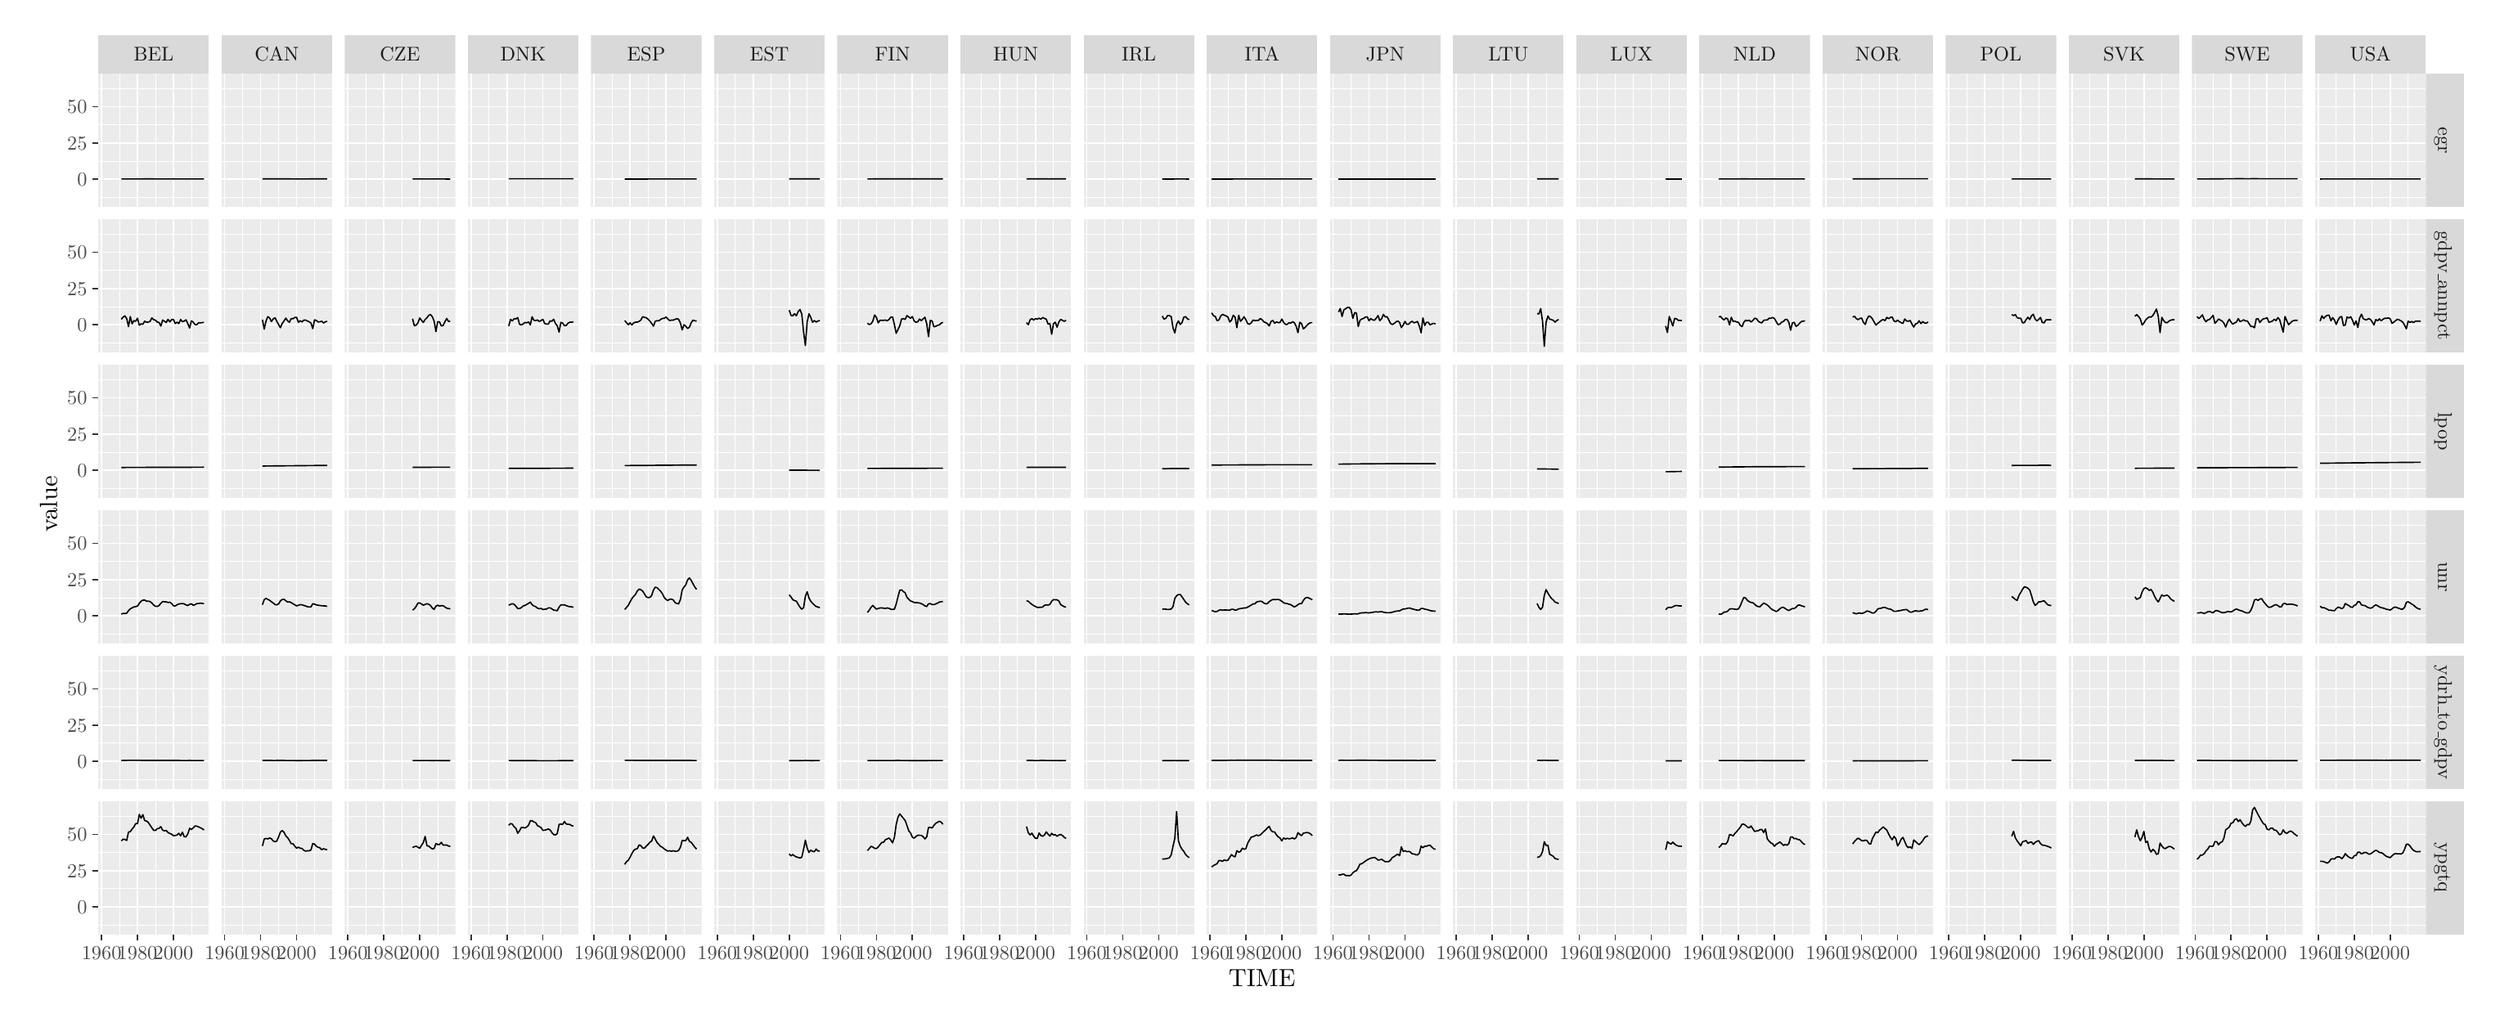
\begin{tikzpicture}[x=1pt,y=1pt]
\definecolor{fillColor}{RGB}{255,255,255}
\path[use as bounding box,fill=fillColor,fill opacity=0.00] (0,0) rectangle (1084.05,433.62);
\begin{scope}
\path[clip] (  0.00,  0.00) rectangle (1084.05,433.62);
\definecolor{drawColor}{RGB}{255,255,255}
\definecolor{fillColor}{RGB}{255,255,255}

\path[draw=drawColor,line width= 0.6pt,line join=round,line cap=round,fill=fillColor] (  0.00,  0.00) rectangle (1084.05,433.62);
\end{scope}
\begin{scope}
\path[clip] ( 33.42,411.06) rectangle ( 82.32,428.12);
\definecolor{fillColor}{gray}{0.85}

\path[fill=fillColor] ( 33.42,411.06) rectangle ( 82.32,428.12);
\definecolor{drawColor}{gray}{0.10}

\node[text=drawColor,anchor=base,inner sep=0pt, outer sep=0pt, scale=  0.88] at ( 57.87,416.56) {BEL};
\end{scope}
\begin{scope}
\path[clip] ( 87.82,411.06) rectangle (136.72,428.12);
\definecolor{fillColor}{gray}{0.85}

\path[fill=fillColor] ( 87.82,411.06) rectangle (136.72,428.12);
\definecolor{drawColor}{gray}{0.10}

\node[text=drawColor,anchor=base,inner sep=0pt, outer sep=0pt, scale=  0.88] at (112.27,416.56) {CAN};
\end{scope}
\begin{scope}
\path[clip] (142.22,411.06) rectangle (191.12,428.12);
\definecolor{fillColor}{gray}{0.85}

\path[fill=fillColor] (142.22,411.06) rectangle (191.12,428.12);
\definecolor{drawColor}{gray}{0.10}

\node[text=drawColor,anchor=base,inner sep=0pt, outer sep=0pt, scale=  0.88] at (166.67,416.56) {CZE};
\end{scope}
\begin{scope}
\path[clip] (196.62,411.06) rectangle (245.52,428.12);
\definecolor{fillColor}{gray}{0.85}

\path[fill=fillColor] (196.62,411.06) rectangle (245.52,428.12);
\definecolor{drawColor}{gray}{0.10}

\node[text=drawColor,anchor=base,inner sep=0pt, outer sep=0pt, scale=  0.88] at (221.07,416.56) {DNK};
\end{scope}
\begin{scope}
\path[clip] (251.02,411.06) rectangle (299.91,428.12);
\definecolor{fillColor}{gray}{0.85}

\path[fill=fillColor] (251.02,411.06) rectangle (299.91,428.12);
\definecolor{drawColor}{gray}{0.10}

\node[text=drawColor,anchor=base,inner sep=0pt, outer sep=0pt, scale=  0.88] at (275.47,416.56) {ESP};
\end{scope}
\begin{scope}
\path[clip] (305.41,411.06) rectangle (354.31,428.12);
\definecolor{fillColor}{gray}{0.85}

\path[fill=fillColor] (305.41,411.06) rectangle (354.31,428.12);
\definecolor{drawColor}{gray}{0.10}

\node[text=drawColor,anchor=base,inner sep=0pt, outer sep=0pt, scale=  0.88] at (329.86,416.56) {EST};
\end{scope}
\begin{scope}
\path[clip] (359.81,411.06) rectangle (408.71,428.12);
\definecolor{fillColor}{gray}{0.85}

\path[fill=fillColor] (359.81,411.06) rectangle (408.71,428.12);
\definecolor{drawColor}{gray}{0.10}

\node[text=drawColor,anchor=base,inner sep=0pt, outer sep=0pt, scale=  0.88] at (384.26,416.56) {FIN};
\end{scope}
\begin{scope}
\path[clip] (414.21,411.06) rectangle (463.11,428.12);
\definecolor{fillColor}{gray}{0.85}

\path[fill=fillColor] (414.21,411.06) rectangle (463.11,428.12);
\definecolor{drawColor}{gray}{0.10}

\node[text=drawColor,anchor=base,inner sep=0pt, outer sep=0pt, scale=  0.88] at (438.66,416.56) {HUN};
\end{scope}
\begin{scope}
\path[clip] (468.61,411.06) rectangle (517.51,428.12);
\definecolor{fillColor}{gray}{0.85}

\path[fill=fillColor] (468.61,411.06) rectangle (517.51,428.12);
\definecolor{drawColor}{gray}{0.10}

\node[text=drawColor,anchor=base,inner sep=0pt, outer sep=0pt, scale=  0.88] at (493.06,416.56) {IRL};
\end{scope}
\begin{scope}
\path[clip] (523.01,411.06) rectangle (571.91,428.12);
\definecolor{fillColor}{gray}{0.85}

\path[fill=fillColor] (523.01,411.06) rectangle (571.91,428.12);
\definecolor{drawColor}{gray}{0.10}

\node[text=drawColor,anchor=base,inner sep=0pt, outer sep=0pt, scale=  0.88] at (547.46,416.56) {ITA};
\end{scope}
\begin{scope}
\path[clip] (577.41,411.06) rectangle (626.30,428.12);
\definecolor{fillColor}{gray}{0.85}

\path[fill=fillColor] (577.41,411.06) rectangle (626.30,428.12);
\definecolor{drawColor}{gray}{0.10}

\node[text=drawColor,anchor=base,inner sep=0pt, outer sep=0pt, scale=  0.88] at (601.85,416.56) {JPN};
\end{scope}
\begin{scope}
\path[clip] (631.80,411.06) rectangle (680.70,428.12);
\definecolor{fillColor}{gray}{0.85}

\path[fill=fillColor] (631.80,411.06) rectangle (680.70,428.12);
\definecolor{drawColor}{gray}{0.10}

\node[text=drawColor,anchor=base,inner sep=0pt, outer sep=0pt, scale=  0.88] at (656.25,416.56) {LTU};
\end{scope}
\begin{scope}
\path[clip] (686.20,411.06) rectangle (735.10,428.12);
\definecolor{fillColor}{gray}{0.85}

\path[fill=fillColor] (686.20,411.06) rectangle (735.10,428.12);
\definecolor{drawColor}{gray}{0.10}

\node[text=drawColor,anchor=base,inner sep=0pt, outer sep=0pt, scale=  0.88] at (710.65,416.56) {LUX};
\end{scope}
\begin{scope}
\path[clip] (740.60,411.06) rectangle (789.50,428.12);
\definecolor{fillColor}{gray}{0.85}

\path[fill=fillColor] (740.60,411.06) rectangle (789.50,428.12);
\definecolor{drawColor}{gray}{0.10}

\node[text=drawColor,anchor=base,inner sep=0pt, outer sep=0pt, scale=  0.88] at (765.05,416.56) {NLD};
\end{scope}
\begin{scope}
\path[clip] (795.00,411.06) rectangle (843.90,428.12);
\definecolor{fillColor}{gray}{0.85}

\path[fill=fillColor] (795.00,411.06) rectangle (843.90,428.12);
\definecolor{drawColor}{gray}{0.10}

\node[text=drawColor,anchor=base,inner sep=0pt, outer sep=0pt, scale=  0.88] at (819.45,416.56) {NOR};
\end{scope}
\begin{scope}
\path[clip] (849.40,411.06) rectangle (898.29,428.12);
\definecolor{fillColor}{gray}{0.85}

\path[fill=fillColor] (849.40,411.06) rectangle (898.29,428.12);
\definecolor{drawColor}{gray}{0.10}

\node[text=drawColor,anchor=base,inner sep=0pt, outer sep=0pt, scale=  0.88] at (873.85,416.56) {POL};
\end{scope}
\begin{scope}
\path[clip] (903.79,411.06) rectangle (952.69,428.12);
\definecolor{fillColor}{gray}{0.85}

\path[fill=fillColor] (903.79,411.06) rectangle (952.69,428.12);
\definecolor{drawColor}{gray}{0.10}

\node[text=drawColor,anchor=base,inner sep=0pt, outer sep=0pt, scale=  0.88] at (928.24,416.56) {SVK};
\end{scope}
\begin{scope}
\path[clip] (958.19,411.06) rectangle (1007.09,428.12);
\definecolor{fillColor}{gray}{0.85}

\path[fill=fillColor] (958.19,411.06) rectangle (1007.09,428.12);
\definecolor{drawColor}{gray}{0.10}

\node[text=drawColor,anchor=base,inner sep=0pt, outer sep=0pt, scale=  0.88] at (982.64,416.56) {SWE};
\end{scope}
\begin{scope}
\path[clip] (1012.59,411.06) rectangle (1061.49,428.12);
\definecolor{fillColor}{gray}{0.85}

\path[fill=fillColor] (1012.59,411.06) rectangle (1061.49,428.12);
\definecolor{drawColor}{gray}{0.10}

\node[text=drawColor,anchor=base,inner sep=0pt, outer sep=0pt, scale=  0.88] at (1037.04,416.56) {USA};
\end{scope}
\begin{scope}
\path[clip] ( 33.42,352.25) rectangle ( 82.32,411.06);
\definecolor{fillColor}{gray}{0.92}

\path[fill=fillColor] ( 33.42,352.25) rectangle ( 82.32,411.06);
\definecolor{drawColor}{RGB}{255,255,255}

\path[draw=drawColor,line width= 0.3pt,line join=round] ( 33.42,356.40) --
	( 82.32,356.40);

\path[draw=drawColor,line width= 0.3pt,line join=round] ( 33.42,372.43) --
	( 82.32,372.43);

\path[draw=drawColor,line width= 0.3pt,line join=round] ( 33.42,388.46) --
	( 82.32,388.46);

\path[draw=drawColor,line width= 0.3pt,line join=round] ( 33.42,404.49) --
	( 82.32,404.49);

\path[draw=drawColor,line width= 0.3pt,line join=round] ( 42.79,352.25) --
	( 42.79,411.06);

\path[draw=drawColor,line width= 0.3pt,line join=round] ( 58.67,352.25) --
	( 58.67,411.06);

\path[draw=drawColor,line width= 0.3pt,line join=round] ( 74.54,352.25) --
	( 74.54,411.06);

\path[draw=drawColor,line width= 0.6pt,line join=round] ( 33.42,364.42) --
	( 82.32,364.42);

\path[draw=drawColor,line width= 0.6pt,line join=round] ( 33.42,380.45) --
	( 82.32,380.45);

\path[draw=drawColor,line width= 0.6pt,line join=round] ( 33.42,396.48) --
	( 82.32,396.48);

\path[draw=drawColor,line width= 0.6pt,line join=round] ( 34.85,352.25) --
	( 34.85,411.06);

\path[draw=drawColor,line width= 0.6pt,line join=round] ( 50.73,352.25) --
	( 50.73,411.06);

\path[draw=drawColor,line width= 0.6pt,line join=round] ( 66.60,352.25) --
	( 66.60,411.06);
\definecolor{drawColor}{RGB}{0,0,0}

\path[draw=drawColor,line width= 0.6pt,line join=round] ( 43.58,364.51) --
	( 44.38,364.51) --
	( 45.17,364.51) --
	( 45.97,364.51) --
	( 46.76,364.52) --
	( 47.55,364.52) --
	( 48.35,364.53) --
	( 49.14,364.53) --
	( 49.93,364.54) --
	( 50.73,364.54) --
	( 51.52,364.54) --
	( 52.32,364.54) --
	( 53.11,364.54) --
	( 53.90,364.55) --
	( 54.70,364.55) --
	( 55.49,364.55) --
	( 56.29,364.55) --
	( 57.08,364.55) --
	( 57.87,364.54) --
	( 58.67,364.54) --
	( 59.46,364.54) --
	( 60.25,364.54) --
	( 61.05,364.54) --
	( 61.84,364.54) --
	( 62.64,364.54) --
	( 63.43,364.54) --
	( 64.22,364.53) --
	( 65.02,364.53) --
	( 65.81,364.53) --
	( 66.60,364.53) --
	( 67.40,364.53) --
	( 68.19,364.53) --
	( 68.99,364.54) --
	( 69.78,364.54) --
	( 70.57,364.54) --
	( 71.37,364.54) --
	( 72.16,364.54) --
	( 72.96,364.54) --
	( 73.75,364.54) --
	( 74.54,364.54) --
	( 75.34,364.54) --
	( 76.13,364.54) --
	( 76.92,364.54) --
	( 77.72,364.54) --
	( 78.51,364.53) --
	( 79.31,364.53) --
	( 80.10,364.53);
\end{scope}
\begin{scope}
\path[clip] ( 33.42,287.94) rectangle ( 82.32,346.75);
\definecolor{fillColor}{gray}{0.92}

\path[fill=fillColor] ( 33.42,287.94) rectangle ( 82.32,346.75);
\definecolor{drawColor}{RGB}{255,255,255}

\path[draw=drawColor,line width= 0.3pt,line join=round] ( 33.42,292.09) --
	( 82.32,292.09);

\path[draw=drawColor,line width= 0.3pt,line join=round] ( 33.42,308.12) --
	( 82.32,308.12);

\path[draw=drawColor,line width= 0.3pt,line join=round] ( 33.42,324.15) --
	( 82.32,324.15);

\path[draw=drawColor,line width= 0.3pt,line join=round] ( 33.42,340.18) --
	( 82.32,340.18);

\path[draw=drawColor,line width= 0.3pt,line join=round] ( 42.79,287.94) --
	( 42.79,346.75);

\path[draw=drawColor,line width= 0.3pt,line join=round] ( 58.67,287.94) --
	( 58.67,346.75);

\path[draw=drawColor,line width= 0.3pt,line join=round] ( 74.54,287.94) --
	( 74.54,346.75);

\path[draw=drawColor,line width= 0.6pt,line join=round] ( 33.42,300.11) --
	( 82.32,300.11);

\path[draw=drawColor,line width= 0.6pt,line join=round] ( 33.42,316.14) --
	( 82.32,316.14);

\path[draw=drawColor,line width= 0.6pt,line join=round] ( 33.42,332.17) --
	( 82.32,332.17);

\path[draw=drawColor,line width= 0.6pt,line join=round] ( 34.85,287.94) --
	( 34.85,346.75);

\path[draw=drawColor,line width= 0.6pt,line join=round] ( 50.73,287.94) --
	( 50.73,346.75);

\path[draw=drawColor,line width= 0.6pt,line join=round] ( 66.60,287.94) --
	( 66.60,346.75);
\definecolor{drawColor}{RGB}{0,0,0}

\path[draw=drawColor,line width= 0.6pt,line join=round] ( 43.58,302.51) --
	( 44.38,303.48) --
	( 45.17,304.03) --
	( 45.97,302.80) --
	( 46.76,299.26) --
	( 47.55,303.73) --
	( 48.35,300.51) --
	( 49.14,301.93) --
	( 49.93,301.61) --
	( 50.73,302.98) --
	( 51.52,299.93) --
	( 52.32,300.49) --
	( 53.11,300.31) --
	( 53.90,301.69) --
	( 54.70,301.17) --
	( 55.49,301.28) --
	( 56.29,301.59) --
	( 57.08,303.14) --
	( 57.87,302.33) --
	( 58.67,302.12) --
	( 59.46,301.28) --
	( 60.25,301.09) --
	( 61.05,299.49) --
	( 61.84,302.18) --
	( 62.64,301.64) --
	( 63.43,301.13) --
	( 64.22,302.49) --
	( 65.02,301.37) --
	( 65.81,302.39) --
	( 66.60,302.44) --
	( 67.40,300.63) --
	( 68.19,301.25) --
	( 68.99,300.60) --
	( 69.78,302.44) --
	( 70.57,301.45) --
	( 71.37,301.71) --
	( 72.16,302.29) --
	( 72.96,300.59) --
	( 73.75,298.64) --
	( 74.54,301.84) --
	( 75.34,301.26) --
	( 76.13,300.20) --
	( 76.92,300.12) --
	( 77.72,300.97) --
	( 78.51,300.94) --
	( 79.31,301.05) --
	( 80.10,301.16);
\end{scope}
\begin{scope}
\path[clip] ( 33.42,223.62) rectangle ( 82.32,282.44);
\definecolor{fillColor}{gray}{0.92}

\path[fill=fillColor] ( 33.42,223.62) rectangle ( 82.32,282.44);
\definecolor{drawColor}{RGB}{255,255,255}

\path[draw=drawColor,line width= 0.3pt,line join=round] ( 33.42,227.78) --
	( 82.32,227.78);

\path[draw=drawColor,line width= 0.3pt,line join=round] ( 33.42,243.81) --
	( 82.32,243.81);

\path[draw=drawColor,line width= 0.3pt,line join=round] ( 33.42,259.84) --
	( 82.32,259.84);

\path[draw=drawColor,line width= 0.3pt,line join=round] ( 33.42,275.87) --
	( 82.32,275.87);

\path[draw=drawColor,line width= 0.3pt,line join=round] ( 42.79,223.62) --
	( 42.79,282.44);

\path[draw=drawColor,line width= 0.3pt,line join=round] ( 58.67,223.62) --
	( 58.67,282.44);

\path[draw=drawColor,line width= 0.3pt,line join=round] ( 74.54,223.62) --
	( 74.54,282.44);

\path[draw=drawColor,line width= 0.6pt,line join=round] ( 33.42,235.80) --
	( 82.32,235.80);

\path[draw=drawColor,line width= 0.6pt,line join=round] ( 33.42,251.82) --
	( 82.32,251.82);

\path[draw=drawColor,line width= 0.6pt,line join=round] ( 33.42,267.85) --
	( 82.32,267.85);

\path[draw=drawColor,line width= 0.6pt,line join=round] ( 34.85,223.62) --
	( 34.85,282.44);

\path[draw=drawColor,line width= 0.6pt,line join=round] ( 50.73,223.62) --
	( 50.73,282.44);

\path[draw=drawColor,line width= 0.6pt,line join=round] ( 66.60,223.62) --
	( 66.60,282.44);
\definecolor{drawColor}{RGB}{0,0,0}

\path[draw=drawColor,line width= 0.6pt,line join=round] ( 43.58,237.04) --
	( 44.38,237.04) --
	( 45.17,237.04) --
	( 45.97,237.05) --
	( 46.76,237.05) --
	( 47.55,237.06) --
	( 48.35,237.06) --
	( 49.14,237.06) --
	( 49.93,237.07) --
	( 50.73,237.07) --
	( 51.52,237.07) --
	( 52.32,237.07) --
	( 53.11,237.07) --
	( 53.90,237.07) --
	( 54.70,237.08) --
	( 55.49,237.08) --
	( 56.29,237.08) --
	( 57.08,237.08) --
	( 57.87,237.08) --
	( 58.67,237.09) --
	( 59.46,237.09) --
	( 60.25,237.09) --
	( 61.05,237.10) --
	( 61.84,237.10) --
	( 62.64,237.10) --
	( 63.43,237.10) --
	( 64.22,237.10) --
	( 65.02,237.10) --
	( 65.81,237.10) --
	( 66.60,237.10) --
	( 67.40,237.10) --
	( 68.19,237.11) --
	( 68.99,237.11) --
	( 69.78,237.11) --
	( 70.57,237.11) --
	( 71.37,237.12) --
	( 72.16,237.12) --
	( 72.96,237.13) --
	( 73.75,237.13) --
	( 74.54,237.13) --
	( 75.34,237.14) --
	( 76.13,237.15) --
	( 76.92,237.15) --
	( 77.72,237.15) --
	( 78.51,237.16) --
	( 79.31,237.16) --
	( 80.10,237.17);
\end{scope}
\begin{scope}
\path[clip] ( 33.42,159.31) rectangle ( 82.32,218.12);
\definecolor{fillColor}{gray}{0.92}

\path[fill=fillColor] ( 33.42,159.31) rectangle ( 82.32,218.12);
\definecolor{drawColor}{RGB}{255,255,255}

\path[draw=drawColor,line width= 0.3pt,line join=round] ( 33.42,163.47) --
	( 82.32,163.47);

\path[draw=drawColor,line width= 0.3pt,line join=round] ( 33.42,179.50) --
	( 82.32,179.50);

\path[draw=drawColor,line width= 0.3pt,line join=round] ( 33.42,195.53) --
	( 82.32,195.53);

\path[draw=drawColor,line width= 0.3pt,line join=round] ( 33.42,211.56) --
	( 82.32,211.56);

\path[draw=drawColor,line width= 0.3pt,line join=round] ( 42.79,159.31) --
	( 42.79,218.12);

\path[draw=drawColor,line width= 0.3pt,line join=round] ( 58.67,159.31) --
	( 58.67,218.12);

\path[draw=drawColor,line width= 0.3pt,line join=round] ( 74.54,159.31) --
	( 74.54,218.12);

\path[draw=drawColor,line width= 0.6pt,line join=round] ( 33.42,171.48) --
	( 82.32,171.48);

\path[draw=drawColor,line width= 0.6pt,line join=round] ( 33.42,187.51) --
	( 82.32,187.51);

\path[draw=drawColor,line width= 0.6pt,line join=round] ( 33.42,203.54) --
	( 82.32,203.54);

\path[draw=drawColor,line width= 0.6pt,line join=round] ( 34.85,159.31) --
	( 34.85,218.12);

\path[draw=drawColor,line width= 0.6pt,line join=round] ( 50.73,159.31) --
	( 50.73,218.12);

\path[draw=drawColor,line width= 0.6pt,line join=round] ( 66.60,159.31) --
	( 66.60,218.12);
\definecolor{drawColor}{RGB}{0,0,0}

\path[draw=drawColor,line width= 0.6pt,line join=round] ( 43.58,172.24) --
	( 44.38,172.50) --
	( 45.17,172.51) --
	( 45.97,172.64) --
	( 46.76,173.75) --
	( 47.55,174.55) --
	( 48.35,175.00) --
	( 49.14,175.38) --
	( 49.93,175.55) --
	( 50.73,175.77) --
	( 51.52,176.99) --
	( 52.32,177.94) --
	( 53.11,178.38) --
	( 53.90,178.41) --
	( 54.70,177.97) --
	( 55.49,177.93) --
	( 56.29,177.78) --
	( 57.08,177.14) --
	( 57.87,176.22) --
	( 58.67,175.68) --
	( 59.46,175.61) --
	( 60.25,176.03) --
	( 61.05,177.01) --
	( 61.84,177.74) --
	( 62.64,177.70) --
	( 63.43,177.61) --
	( 64.22,177.40) --
	( 65.02,177.47) --
	( 65.81,176.90) --
	( 66.60,175.93) --
	( 67.40,175.79) --
	( 68.19,176.37) --
	( 68.99,176.71) --
	( 69.78,176.82) --
	( 70.57,176.88) --
	( 71.37,176.76) --
	( 72.16,176.29) --
	( 72.96,176.03) --
	( 73.75,176.53) --
	( 74.54,176.77) --
	( 75.34,176.12) --
	( 76.13,176.38) --
	( 76.92,176.87) --
	( 77.72,176.92) --
	( 78.51,177.08) --
	( 79.31,176.98) --
	( 80.10,176.80);
\end{scope}
\begin{scope}
\path[clip] ( 33.42, 95.00) rectangle ( 82.32,153.81);
\definecolor{fillColor}{gray}{0.92}

\path[fill=fillColor] ( 33.42, 95.00) rectangle ( 82.32,153.81);
\definecolor{drawColor}{RGB}{255,255,255}

\path[draw=drawColor,line width= 0.3pt,line join=round] ( 33.42, 99.16) --
	( 82.32, 99.16);

\path[draw=drawColor,line width= 0.3pt,line join=round] ( 33.42,115.19) --
	( 82.32,115.19);

\path[draw=drawColor,line width= 0.3pt,line join=round] ( 33.42,131.22) --
	( 82.32,131.22);

\path[draw=drawColor,line width= 0.3pt,line join=round] ( 33.42,147.25) --
	( 82.32,147.25);

\path[draw=drawColor,line width= 0.3pt,line join=round] ( 42.79, 95.00) --
	( 42.79,153.81);

\path[draw=drawColor,line width= 0.3pt,line join=round] ( 58.67, 95.00) --
	( 58.67,153.81);

\path[draw=drawColor,line width= 0.3pt,line join=round] ( 74.54, 95.00) --
	( 74.54,153.81);

\path[draw=drawColor,line width= 0.6pt,line join=round] ( 33.42,107.17) --
	( 82.32,107.17);

\path[draw=drawColor,line width= 0.6pt,line join=round] ( 33.42,123.20) --
	( 82.32,123.20);

\path[draw=drawColor,line width= 0.6pt,line join=round] ( 33.42,139.23) --
	( 82.32,139.23);

\path[draw=drawColor,line width= 0.6pt,line join=round] ( 34.85, 95.00) --
	( 34.85,153.81);

\path[draw=drawColor,line width= 0.6pt,line join=round] ( 50.73, 95.00) --
	( 50.73,153.81);

\path[draw=drawColor,line width= 0.6pt,line join=round] ( 66.60, 95.00) --
	( 66.60,153.81);
\definecolor{drawColor}{RGB}{0,0,0}

\path[draw=drawColor,line width= 0.6pt,line join=round] ( 43.58,107.58) --
	( 44.38,107.59) --
	( 45.17,107.59) --
	( 45.97,107.59) --
	( 46.76,107.60) --
	( 47.55,107.60) --
	( 48.35,107.60) --
	( 49.14,107.60) --
	( 49.93,107.60) --
	( 50.73,107.60) --
	( 51.52,107.60) --
	( 52.32,107.59) --
	( 53.11,107.58) --
	( 53.90,107.57) --
	( 54.70,107.56) --
	( 55.49,107.57) --
	( 56.29,107.56) --
	( 57.08,107.56) --
	( 57.87,107.56) --
	( 58.67,107.56) --
	( 59.46,107.57) --
	( 60.25,107.58) --
	( 61.05,107.58) --
	( 61.84,107.57) --
	( 62.64,107.59) --
	( 63.43,107.58) --
	( 64.22,107.57) --
	( 65.02,107.57) --
	( 65.81,107.56) --
	( 66.60,107.55) --
	( 67.40,107.56) --
	( 68.19,107.55) --
	( 68.99,107.55) --
	( 69.78,107.53) --
	( 70.57,107.53) --
	( 71.37,107.53) --
	( 72.16,107.52) --
	( 72.96,107.53) --
	( 73.75,107.54) --
	( 74.54,107.53) --
	( 75.34,107.52) --
	( 76.13,107.52) --
	( 76.92,107.52) --
	( 77.72,107.51) --
	( 78.51,107.51) --
	( 79.31,107.51) --
	( 80.10,107.51);
\end{scope}
\begin{scope}
\path[clip] ( 33.42, 30.69) rectangle ( 82.32, 89.50);
\definecolor{fillColor}{gray}{0.92}

\path[fill=fillColor] ( 33.42, 30.69) rectangle ( 82.32, 89.50);
\definecolor{drawColor}{RGB}{255,255,255}

\path[draw=drawColor,line width= 0.3pt,line join=round] ( 33.42, 34.84) --
	( 82.32, 34.84);

\path[draw=drawColor,line width= 0.3pt,line join=round] ( 33.42, 50.87) --
	( 82.32, 50.87);

\path[draw=drawColor,line width= 0.3pt,line join=round] ( 33.42, 66.90) --
	( 82.32, 66.90);

\path[draw=drawColor,line width= 0.3pt,line join=round] ( 33.42, 82.93) --
	( 82.32, 82.93);

\path[draw=drawColor,line width= 0.3pt,line join=round] ( 42.79, 30.69) --
	( 42.79, 89.50);

\path[draw=drawColor,line width= 0.3pt,line join=round] ( 58.67, 30.69) --
	( 58.67, 89.50);

\path[draw=drawColor,line width= 0.3pt,line join=round] ( 74.54, 30.69) --
	( 74.54, 89.50);

\path[draw=drawColor,line width= 0.6pt,line join=round] ( 33.42, 42.86) --
	( 82.32, 42.86);

\path[draw=drawColor,line width= 0.6pt,line join=round] ( 33.42, 58.89) --
	( 82.32, 58.89);

\path[draw=drawColor,line width= 0.6pt,line join=round] ( 33.42, 74.92) --
	( 82.32, 74.92);

\path[draw=drawColor,line width= 0.6pt,line join=round] ( 34.85, 30.69) --
	( 34.85, 89.50);

\path[draw=drawColor,line width= 0.6pt,line join=round] ( 50.73, 30.69) --
	( 50.73, 89.50);

\path[draw=drawColor,line width= 0.6pt,line join=round] ( 66.60, 30.69) --
	( 66.60, 89.50);
\definecolor{drawColor}{RGB}{0,0,0}

\path[draw=drawColor,line width= 0.6pt,line join=round] ( 43.58, 71.97) --
	( 44.38, 72.77) --
	( 45.17, 72.63) --
	( 45.97, 72.20) --
	( 46.76, 75.90) --
	( 47.55, 76.09) --
	( 48.35, 77.22) --
	( 49.14, 78.18) --
	( 49.93, 79.65) --
	( 50.73, 79.59) --
	( 51.52, 83.71) --
	( 52.32, 82.02) --
	( 53.11, 83.61) --
	( 53.90, 80.99) --
	( 54.70, 80.78) --
	( 55.49, 80.19) --
	( 56.29, 78.93) --
	( 57.08, 77.80) --
	( 57.87, 76.67) --
	( 58.67, 76.65) --
	( 59.46, 77.39) --
	( 60.25, 77.56) --
	( 61.05, 78.30) --
	( 61.84, 76.76) --
	( 62.64, 76.45) --
	( 63.43, 76.63) --
	( 64.22, 75.71) --
	( 65.02, 75.28) --
	( 65.81, 74.96) --
	( 66.60, 74.31) --
	( 67.40, 74.40) --
	( 68.19, 74.60) --
	( 68.99, 75.38) --
	( 69.78, 74.23) --
	( 70.57, 75.84) --
	( 71.37, 73.87) --
	( 72.16, 73.79) --
	( 72.96, 75.09) --
	( 73.75, 77.57) --
	( 74.54, 77.03) --
	( 75.34, 77.75) --
	( 76.13, 78.63) --
	( 76.92, 78.50) --
	( 77.72, 78.19) --
	( 78.51, 77.83) --
	( 79.31, 77.41) --
	( 80.10, 76.82);
\end{scope}
\begin{scope}
\path[clip] ( 87.82,352.25) rectangle (136.72,411.06);
\definecolor{fillColor}{gray}{0.92}

\path[fill=fillColor] ( 87.82,352.25) rectangle (136.72,411.06);
\definecolor{drawColor}{RGB}{255,255,255}

\path[draw=drawColor,line width= 0.3pt,line join=round] ( 87.82,356.40) --
	(136.72,356.40);

\path[draw=drawColor,line width= 0.3pt,line join=round] ( 87.82,372.43) --
	(136.72,372.43);

\path[draw=drawColor,line width= 0.3pt,line join=round] ( 87.82,388.46) --
	(136.72,388.46);

\path[draw=drawColor,line width= 0.3pt,line join=round] ( 87.82,404.49) --
	(136.72,404.49);

\path[draw=drawColor,line width= 0.3pt,line join=round] ( 97.19,352.25) --
	( 97.19,411.06);

\path[draw=drawColor,line width= 0.3pt,line join=round] (113.06,352.25) --
	(113.06,411.06);

\path[draw=drawColor,line width= 0.3pt,line join=round] (128.94,352.25) --
	(128.94,411.06);

\path[draw=drawColor,line width= 0.6pt,line join=round] ( 87.82,364.42) --
	(136.72,364.42);

\path[draw=drawColor,line width= 0.6pt,line join=round] ( 87.82,380.45) --
	(136.72,380.45);

\path[draw=drawColor,line width= 0.6pt,line join=round] ( 87.82,396.48) --
	(136.72,396.48);

\path[draw=drawColor,line width= 0.6pt,line join=round] ( 89.25,352.25) --
	( 89.25,411.06);

\path[draw=drawColor,line width= 0.6pt,line join=round] (105.13,352.25) --
	(105.13,411.06);

\path[draw=drawColor,line width= 0.6pt,line join=round] (121.00,352.25) --
	(121.00,411.06);
\definecolor{drawColor}{RGB}{0,0,0}

\path[draw=drawColor,line width= 0.6pt,line join=round] (105.92,364.56) --
	(106.71,364.57) --
	(107.51,364.57) --
	(108.30,364.56) --
	(109.10,364.56) --
	(109.89,364.56) --
	(110.68,364.56) --
	(111.48,364.55) --
	(112.27,364.55) --
	(113.06,364.55) --
	(113.86,364.56) --
	(114.65,364.56) --
	(115.45,364.56) --
	(116.24,364.56) --
	(117.03,364.55) --
	(117.83,364.55) --
	(118.62,364.54) --
	(119.42,364.54) --
	(120.21,364.54) --
	(121.00,364.54) --
	(121.80,364.54) --
	(122.59,364.54) --
	(123.38,364.54) --
	(124.18,364.54) --
	(124.97,364.54) --
	(125.77,364.54) --
	(126.56,364.54) --
	(127.35,364.55) --
	(128.15,364.55) --
	(128.94,364.55) --
	(129.73,364.55) --
	(130.53,364.55) --
	(131.32,364.55) --
	(132.12,364.55) --
	(132.91,364.55) --
	(133.70,364.55) --
	(134.50,364.55);
\end{scope}
\begin{scope}
\path[clip] ( 87.82,287.94) rectangle (136.72,346.75);
\definecolor{fillColor}{gray}{0.92}

\path[fill=fillColor] ( 87.82,287.94) rectangle (136.72,346.75);
\definecolor{drawColor}{RGB}{255,255,255}

\path[draw=drawColor,line width= 0.3pt,line join=round] ( 87.82,292.09) --
	(136.72,292.09);

\path[draw=drawColor,line width= 0.3pt,line join=round] ( 87.82,308.12) --
	(136.72,308.12);

\path[draw=drawColor,line width= 0.3pt,line join=round] ( 87.82,324.15) --
	(136.72,324.15);

\path[draw=drawColor,line width= 0.3pt,line join=round] ( 87.82,340.18) --
	(136.72,340.18);

\path[draw=drawColor,line width= 0.3pt,line join=round] ( 97.19,287.94) --
	( 97.19,346.75);

\path[draw=drawColor,line width= 0.3pt,line join=round] (113.06,287.94) --
	(113.06,346.75);

\path[draw=drawColor,line width= 0.3pt,line join=round] (128.94,287.94) --
	(128.94,346.75);

\path[draw=drawColor,line width= 0.6pt,line join=round] ( 87.82,300.11) --
	(136.72,300.11);

\path[draw=drawColor,line width= 0.6pt,line join=round] ( 87.82,316.14) --
	(136.72,316.14);

\path[draw=drawColor,line width= 0.6pt,line join=round] ( 87.82,332.17) --
	(136.72,332.17);

\path[draw=drawColor,line width= 0.6pt,line join=round] ( 89.25,287.94) --
	( 89.25,346.75);

\path[draw=drawColor,line width= 0.6pt,line join=round] (105.13,287.94) --
	(105.13,346.75);

\path[draw=drawColor,line width= 0.6pt,line join=round] (121.00,287.94) --
	(121.00,346.75);
\definecolor{drawColor}{RGB}{0,0,0}

\path[draw=drawColor,line width= 0.6pt,line join=round] (105.92,302.35) --
	(106.71,298.17) --
	(107.51,301.75) --
	(108.30,303.68) --
	(109.10,303.11) --
	(109.89,301.52) --
	(110.68,302.70) --
	(111.48,303.14) --
	(112.27,301.63) --
	(113.06,300.19) --
	(113.86,298.75) --
	(114.65,300.65) --
	(115.45,301.78) --
	(116.24,303.03) --
	(117.03,301.86) --
	(117.83,301.18) --
	(118.62,302.83) --
	(119.42,302.76) --
	(120.21,303.31) --
	(121.00,303.39) --
	(121.80,301.19) --
	(122.59,301.90) --
	(123.38,301.34) --
	(124.18,302.12) --
	(124.97,302.14) --
	(125.77,301.79) --
	(126.56,301.39) --
	(127.35,300.86) --
	(128.15,298.37) --
	(128.94,302.27) --
	(129.73,302.01) --
	(130.53,301.34) --
	(131.32,301.39) --
	(132.12,301.67) --
	(132.91,300.86) --
	(133.70,301.39) --
	(134.50,301.60);
\end{scope}
\begin{scope}
\path[clip] ( 87.82,223.62) rectangle (136.72,282.44);
\definecolor{fillColor}{gray}{0.92}

\path[fill=fillColor] ( 87.82,223.62) rectangle (136.72,282.44);
\definecolor{drawColor}{RGB}{255,255,255}

\path[draw=drawColor,line width= 0.3pt,line join=round] ( 87.82,227.78) --
	(136.72,227.78);

\path[draw=drawColor,line width= 0.3pt,line join=round] ( 87.82,243.81) --
	(136.72,243.81);

\path[draw=drawColor,line width= 0.3pt,line join=round] ( 87.82,259.84) --
	(136.72,259.84);

\path[draw=drawColor,line width= 0.3pt,line join=round] ( 87.82,275.87) --
	(136.72,275.87);

\path[draw=drawColor,line width= 0.3pt,line join=round] ( 97.19,223.62) --
	( 97.19,282.44);

\path[draw=drawColor,line width= 0.3pt,line join=round] (113.06,223.62) --
	(113.06,282.44);

\path[draw=drawColor,line width= 0.3pt,line join=round] (128.94,223.62) --
	(128.94,282.44);

\path[draw=drawColor,line width= 0.6pt,line join=round] ( 87.82,235.80) --
	(136.72,235.80);

\path[draw=drawColor,line width= 0.6pt,line join=round] ( 87.82,251.82) --
	(136.72,251.82);

\path[draw=drawColor,line width= 0.6pt,line join=round] ( 87.82,267.85) --
	(136.72,267.85);

\path[draw=drawColor,line width= 0.6pt,line join=round] ( 89.25,223.62) --
	( 89.25,282.44);

\path[draw=drawColor,line width= 0.6pt,line join=round] (105.13,223.62) --
	(105.13,282.44);

\path[draw=drawColor,line width= 0.6pt,line join=round] (121.00,223.62) --
	(121.00,282.44);
\definecolor{drawColor}{RGB}{0,0,0}

\path[draw=drawColor,line width= 0.6pt,line join=round] (105.92,237.66) --
	(106.71,237.67) --
	(107.51,237.68) --
	(108.30,237.69) --
	(109.10,237.69) --
	(109.89,237.70) --
	(110.68,237.71) --
	(111.48,237.72) --
	(112.27,237.73) --
	(113.06,237.74) --
	(113.86,237.75) --
	(114.65,237.75) --
	(115.45,237.76) --
	(116.24,237.77) --
	(117.03,237.77) --
	(117.83,237.78) --
	(118.62,237.79) --
	(119.42,237.79) --
	(120.21,237.80) --
	(121.00,237.81) --
	(121.80,237.82) --
	(122.59,237.82) --
	(123.38,237.83) --
	(124.18,237.84) --
	(124.97,237.85) --
	(125.77,237.86) --
	(126.56,237.87) --
	(127.35,237.87) --
	(128.15,237.88) --
	(128.94,237.89) --
	(129.73,237.90) --
	(130.53,237.90) --
	(131.32,237.91) --
	(132.12,237.91) --
	(132.91,237.92) --
	(133.70,237.92) --
	(134.50,237.93);
\end{scope}
\begin{scope}
\path[clip] ( 87.82,159.31) rectangle (136.72,218.12);
\definecolor{fillColor}{gray}{0.92}

\path[fill=fillColor] ( 87.82,159.31) rectangle (136.72,218.12);
\definecolor{drawColor}{RGB}{255,255,255}

\path[draw=drawColor,line width= 0.3pt,line join=round] ( 87.82,163.47) --
	(136.72,163.47);

\path[draw=drawColor,line width= 0.3pt,line join=round] ( 87.82,179.50) --
	(136.72,179.50);

\path[draw=drawColor,line width= 0.3pt,line join=round] ( 87.82,195.53) --
	(136.72,195.53);

\path[draw=drawColor,line width= 0.3pt,line join=round] ( 87.82,211.56) --
	(136.72,211.56);

\path[draw=drawColor,line width= 0.3pt,line join=round] ( 97.19,159.31) --
	( 97.19,218.12);

\path[draw=drawColor,line width= 0.3pt,line join=round] (113.06,159.31) --
	(113.06,218.12);

\path[draw=drawColor,line width= 0.3pt,line join=round] (128.94,159.31) --
	(128.94,218.12);

\path[draw=drawColor,line width= 0.6pt,line join=round] ( 87.82,171.48) --
	(136.72,171.48);

\path[draw=drawColor,line width= 0.6pt,line join=round] ( 87.82,187.51) --
	(136.72,187.51);

\path[draw=drawColor,line width= 0.6pt,line join=round] ( 87.82,203.54) --
	(136.72,203.54);

\path[draw=drawColor,line width= 0.6pt,line join=round] ( 89.25,159.31) --
	( 89.25,218.12);

\path[draw=drawColor,line width= 0.6pt,line join=round] (105.13,159.31) --
	(105.13,218.12);

\path[draw=drawColor,line width= 0.6pt,line join=round] (121.00,159.31) --
	(121.00,218.12);
\definecolor{drawColor}{RGB}{0,0,0}

\path[draw=drawColor,line width= 0.6pt,line join=round] (105.92,176.37) --
	(106.71,178.62) --
	(107.51,179.17) --
	(108.30,178.77) --
	(109.10,178.30) --
	(109.89,177.70) --
	(110.68,177.13) --
	(111.48,176.46) --
	(112.27,176.31) --
	(113.06,176.71) --
	(113.86,178.10) --
	(114.65,178.68) --
	(115.45,178.77) --
	(116.24,178.14) --
	(117.03,177.56) --
	(117.83,177.65) --
	(118.62,177.31) --
	(119.42,176.79) --
	(120.21,176.33) --
	(121.00,175.87) --
	(121.80,176.12) --
	(122.59,176.40) --
	(123.38,176.34) --
	(124.18,176.07) --
	(124.97,175.81) --
	(125.77,175.53) --
	(126.56,175.35) --
	(127.35,175.42) --
	(128.15,176.83) --
	(128.94,176.63) --
	(129.73,176.30) --
	(130.53,176.17) --
	(131.32,176.03) --
	(132.12,175.92) --
	(132.91,175.88) --
	(133.70,175.86) --
	(134.50,175.61);
\end{scope}
\begin{scope}
\path[clip] ( 87.82, 95.00) rectangle (136.72,153.81);
\definecolor{fillColor}{gray}{0.92}

\path[fill=fillColor] ( 87.82, 95.00) rectangle (136.72,153.81);
\definecolor{drawColor}{RGB}{255,255,255}

\path[draw=drawColor,line width= 0.3pt,line join=round] ( 87.82, 99.16) --
	(136.72, 99.16);

\path[draw=drawColor,line width= 0.3pt,line join=round] ( 87.82,115.19) --
	(136.72,115.19);

\path[draw=drawColor,line width= 0.3pt,line join=round] ( 87.82,131.22) --
	(136.72,131.22);

\path[draw=drawColor,line width= 0.3pt,line join=round] ( 87.82,147.25) --
	(136.72,147.25);

\path[draw=drawColor,line width= 0.3pt,line join=round] ( 97.19, 95.00) --
	( 97.19,153.81);

\path[draw=drawColor,line width= 0.3pt,line join=round] (113.06, 95.00) --
	(113.06,153.81);

\path[draw=drawColor,line width= 0.3pt,line join=round] (128.94, 95.00) --
	(128.94,153.81);

\path[draw=drawColor,line width= 0.6pt,line join=round] ( 87.82,107.17) --
	(136.72,107.17);

\path[draw=drawColor,line width= 0.6pt,line join=round] ( 87.82,123.20) --
	(136.72,123.20);

\path[draw=drawColor,line width= 0.6pt,line join=round] ( 87.82,139.23) --
	(136.72,139.23);

\path[draw=drawColor,line width= 0.6pt,line join=round] ( 89.25, 95.00) --
	( 89.25,153.81);

\path[draw=drawColor,line width= 0.6pt,line join=round] (105.13, 95.00) --
	(105.13,153.81);

\path[draw=drawColor,line width= 0.6pt,line join=round] (121.00, 95.00) --
	(121.00,153.81);
\definecolor{drawColor}{RGB}{0,0,0}

\path[draw=drawColor,line width= 0.6pt,line join=round] (105.92,107.55) --
	(106.71,107.57) --
	(107.51,107.55) --
	(108.30,107.55) --
	(109.10,107.54) --
	(109.89,107.54) --
	(110.68,107.53) --
	(111.48,107.53) --
	(112.27,107.54) --
	(113.06,107.54) --
	(113.86,107.55) --
	(114.65,107.55) --
	(115.45,107.54) --
	(116.24,107.53) --
	(117.03,107.52) --
	(117.83,107.52) --
	(118.62,107.51) --
	(119.42,107.51) --
	(120.21,107.50) --
	(121.00,107.50) --
	(121.80,107.50) --
	(122.59,107.50) --
	(123.38,107.50) --
	(124.18,107.51) --
	(124.97,107.50) --
	(125.77,107.52) --
	(126.56,107.52) --
	(127.35,107.53) --
	(128.15,107.55) --
	(128.94,107.54) --
	(129.73,107.54) --
	(130.53,107.54) --
	(131.32,107.55) --
	(132.12,107.54) --
	(132.91,107.55) --
	(133.70,107.55) --
	(134.50,107.55);
\end{scope}
\begin{scope}
\path[clip] ( 87.82, 30.69) rectangle (136.72, 89.50);
\definecolor{fillColor}{gray}{0.92}

\path[fill=fillColor] ( 87.82, 30.69) rectangle (136.72, 89.50);
\definecolor{drawColor}{RGB}{255,255,255}

\path[draw=drawColor,line width= 0.3pt,line join=round] ( 87.82, 34.84) --
	(136.72, 34.84);

\path[draw=drawColor,line width= 0.3pt,line join=round] ( 87.82, 50.87) --
	(136.72, 50.87);

\path[draw=drawColor,line width= 0.3pt,line join=round] ( 87.82, 66.90) --
	(136.72, 66.90);

\path[draw=drawColor,line width= 0.3pt,line join=round] ( 87.82, 82.93) --
	(136.72, 82.93);

\path[draw=drawColor,line width= 0.3pt,line join=round] ( 97.19, 30.69) --
	( 97.19, 89.50);

\path[draw=drawColor,line width= 0.3pt,line join=round] (113.06, 30.69) --
	(113.06, 89.50);

\path[draw=drawColor,line width= 0.3pt,line join=round] (128.94, 30.69) --
	(128.94, 89.50);

\path[draw=drawColor,line width= 0.6pt,line join=round] ( 87.82, 42.86) --
	(136.72, 42.86);

\path[draw=drawColor,line width= 0.6pt,line join=round] ( 87.82, 58.89) --
	(136.72, 58.89);

\path[draw=drawColor,line width= 0.6pt,line join=round] ( 87.82, 74.92) --
	(136.72, 74.92);

\path[draw=drawColor,line width= 0.6pt,line join=round] ( 89.25, 30.69) --
	( 89.25, 89.50);

\path[draw=drawColor,line width= 0.6pt,line join=round] (105.13, 30.69) --
	(105.13, 89.50);

\path[draw=drawColor,line width= 0.6pt,line join=round] (121.00, 30.69) --
	(121.00, 89.50);
\definecolor{drawColor}{RGB}{0,0,0}

\path[draw=drawColor,line width= 0.6pt,line join=round] (105.92, 69.78) --
	(106.71, 72.79) --
	(107.51, 73.12) --
	(108.30, 72.88) --
	(109.10, 73.33) --
	(109.89, 72.91) --
	(110.68, 71.98) --
	(111.48, 71.62) --
	(112.27, 71.95) --
	(113.06, 73.76) --
	(113.86, 75.91) --
	(114.65, 76.58) --
	(115.45, 75.84) --
	(116.24, 74.25) --
	(117.03, 73.46) --
	(117.83, 72.22) --
	(118.62, 70.76) --
	(119.42, 70.74) --
	(120.21, 69.66) --
	(121.00, 68.81) --
	(121.80, 69.24) --
	(122.59, 68.77) --
	(123.38, 68.66) --
	(124.18, 67.86) --
	(124.97, 67.49) --
	(125.77, 67.62) --
	(126.56, 67.63) --
	(127.35, 68.00) --
	(128.15, 70.86) --
	(128.94, 70.60) --
	(129.73, 69.61) --
	(130.53, 69.20) --
	(131.32, 68.93) --
	(132.12, 68.11) --
	(132.91, 68.55) --
	(133.70, 68.27) --
	(134.50, 68.13);
\end{scope}
\begin{scope}
\path[clip] (142.22,352.25) rectangle (191.12,411.06);
\definecolor{fillColor}{gray}{0.92}

\path[fill=fillColor] (142.22,352.25) rectangle (191.12,411.06);
\definecolor{drawColor}{RGB}{255,255,255}

\path[draw=drawColor,line width= 0.3pt,line join=round] (142.22,356.40) --
	(191.12,356.40);

\path[draw=drawColor,line width= 0.3pt,line join=round] (142.22,372.43) --
	(191.12,372.43);

\path[draw=drawColor,line width= 0.3pt,line join=round] (142.22,388.46) --
	(191.12,388.46);

\path[draw=drawColor,line width= 0.3pt,line join=round] (142.22,404.49) --
	(191.12,404.49);

\path[draw=drawColor,line width= 0.3pt,line join=round] (151.59,352.25) --
	(151.59,411.06);

\path[draw=drawColor,line width= 0.3pt,line join=round] (167.46,352.25) --
	(167.46,411.06);

\path[draw=drawColor,line width= 0.3pt,line join=round] (183.34,352.25) --
	(183.34,411.06);

\path[draw=drawColor,line width= 0.6pt,line join=round] (142.22,364.42) --
	(191.12,364.42);

\path[draw=drawColor,line width= 0.6pt,line join=round] (142.22,380.45) --
	(191.12,380.45);

\path[draw=drawColor,line width= 0.6pt,line join=round] (142.22,396.48) --
	(191.12,396.48);

\path[draw=drawColor,line width= 0.6pt,line join=round] (143.65,352.25) --
	(143.65,411.06);

\path[draw=drawColor,line width= 0.6pt,line join=round] (159.53,352.25) --
	(159.53,411.06);

\path[draw=drawColor,line width= 0.6pt,line join=round] (175.40,352.25) --
	(175.40,411.06);
\definecolor{drawColor}{RGB}{0,0,0}

\path[draw=drawColor,line width= 0.6pt,line join=round] (172.23,364.51) --
	(173.02,364.51) --
	(173.81,364.51) --
	(174.61,364.51) --
	(175.40,364.51) --
	(176.19,364.51) --
	(176.99,364.51) --
	(177.78,364.51) --
	(178.58,364.51) --
	(179.37,364.51) --
	(180.16,364.51) --
	(180.96,364.51) --
	(181.75,364.51) --
	(182.55,364.51) --
	(183.34,364.51) --
	(184.13,364.51) --
	(184.93,364.51) --
	(185.72,364.51) --
	(186.51,364.51) --
	(187.31,364.50) --
	(188.10,364.50) --
	(188.90,364.50);
\end{scope}
\begin{scope}
\path[clip] (142.22,287.94) rectangle (191.12,346.75);
\definecolor{fillColor}{gray}{0.92}

\path[fill=fillColor] (142.22,287.94) rectangle (191.12,346.75);
\definecolor{drawColor}{RGB}{255,255,255}

\path[draw=drawColor,line width= 0.3pt,line join=round] (142.22,292.09) --
	(191.12,292.09);

\path[draw=drawColor,line width= 0.3pt,line join=round] (142.22,308.12) --
	(191.12,308.12);

\path[draw=drawColor,line width= 0.3pt,line join=round] (142.22,324.15) --
	(191.12,324.15);

\path[draw=drawColor,line width= 0.3pt,line join=round] (142.22,340.18) --
	(191.12,340.18);

\path[draw=drawColor,line width= 0.3pt,line join=round] (151.59,287.94) --
	(151.59,346.75);

\path[draw=drawColor,line width= 0.3pt,line join=round] (167.46,287.94) --
	(167.46,346.75);

\path[draw=drawColor,line width= 0.3pt,line join=round] (183.34,287.94) --
	(183.34,346.75);

\path[draw=drawColor,line width= 0.6pt,line join=round] (142.22,300.11) --
	(191.12,300.11);

\path[draw=drawColor,line width= 0.6pt,line join=round] (142.22,316.14) --
	(191.12,316.14);

\path[draw=drawColor,line width= 0.6pt,line join=round] (142.22,332.17) --
	(191.12,332.17);

\path[draw=drawColor,line width= 0.6pt,line join=round] (143.65,287.94) --
	(143.65,346.75);

\path[draw=drawColor,line width= 0.6pt,line join=round] (159.53,287.94) --
	(159.53,346.75);

\path[draw=drawColor,line width= 0.6pt,line join=round] (175.40,287.94) --
	(175.40,346.75);
\definecolor{drawColor}{RGB}{0,0,0}

\path[draw=drawColor,line width= 0.6pt,line join=round] (172.23,302.78) --
	(173.02,299.66) --
	(173.81,299.91) --
	(174.61,300.92) --
	(175.40,303.09) --
	(176.19,302.06) --
	(176.99,301.11) --
	(177.78,302.41) --
	(178.58,303.18) --
	(179.37,304.28) --
	(180.16,304.64) --
	(180.96,303.64) --
	(181.75,301.74) --
	(182.55,297.09) --
	(183.34,301.48) --
	(184.13,301.37) --
	(184.93,299.58) --
	(185.72,299.77) --
	(186.51,301.38) --
	(187.31,302.89) --
	(188.10,301.60) --
	(188.90,301.65);
\end{scope}
\begin{scope}
\path[clip] (142.22,223.62) rectangle (191.12,282.44);
\definecolor{fillColor}{gray}{0.92}

\path[fill=fillColor] (142.22,223.62) rectangle (191.12,282.44);
\definecolor{drawColor}{RGB}{255,255,255}

\path[draw=drawColor,line width= 0.3pt,line join=round] (142.22,227.78) --
	(191.12,227.78);

\path[draw=drawColor,line width= 0.3pt,line join=round] (142.22,243.81) --
	(191.12,243.81);

\path[draw=drawColor,line width= 0.3pt,line join=round] (142.22,259.84) --
	(191.12,259.84);

\path[draw=drawColor,line width= 0.3pt,line join=round] (142.22,275.87) --
	(191.12,275.87);

\path[draw=drawColor,line width= 0.3pt,line join=round] (151.59,223.62) --
	(151.59,282.44);

\path[draw=drawColor,line width= 0.3pt,line join=round] (167.46,223.62) --
	(167.46,282.44);

\path[draw=drawColor,line width= 0.3pt,line join=round] (183.34,223.62) --
	(183.34,282.44);

\path[draw=drawColor,line width= 0.6pt,line join=round] (142.22,235.80) --
	(191.12,235.80);

\path[draw=drawColor,line width= 0.6pt,line join=round] (142.22,251.82) --
	(191.12,251.82);

\path[draw=drawColor,line width= 0.6pt,line join=round] (142.22,267.85) --
	(191.12,267.85);

\path[draw=drawColor,line width= 0.6pt,line join=round] (143.65,223.62) --
	(143.65,282.44);

\path[draw=drawColor,line width= 0.6pt,line join=round] (159.53,223.62) --
	(159.53,282.44);

\path[draw=drawColor,line width= 0.6pt,line join=round] (175.40,223.62) --
	(175.40,282.44);
\definecolor{drawColor}{RGB}{0,0,0}

\path[draw=drawColor,line width= 0.6pt,line join=round] (172.23,237.12) --
	(173.02,237.13) --
	(173.81,237.13) --
	(174.61,237.13) --
	(175.40,237.13) --
	(176.19,237.13) --
	(176.99,237.13) --
	(177.78,237.13) --
	(178.58,237.13) --
	(179.37,237.13) --
	(180.16,237.13) --
	(180.96,237.14) --
	(181.75,237.14) --
	(182.55,237.15) --
	(183.34,237.15) --
	(184.13,237.15) --
	(184.93,237.15) --
	(185.72,237.15) --
	(186.51,237.15) --
	(187.31,237.14) --
	(188.10,237.14) --
	(188.90,237.14);
\end{scope}
\begin{scope}
\path[clip] (142.22,159.31) rectangle (191.12,218.12);
\definecolor{fillColor}{gray}{0.92}

\path[fill=fillColor] (142.22,159.31) rectangle (191.12,218.12);
\definecolor{drawColor}{RGB}{255,255,255}

\path[draw=drawColor,line width= 0.3pt,line join=round] (142.22,163.47) --
	(191.12,163.47);

\path[draw=drawColor,line width= 0.3pt,line join=round] (142.22,179.50) --
	(191.12,179.50);

\path[draw=drawColor,line width= 0.3pt,line join=round] (142.22,195.53) --
	(191.12,195.53);

\path[draw=drawColor,line width= 0.3pt,line join=round] (142.22,211.56) --
	(191.12,211.56);

\path[draw=drawColor,line width= 0.3pt,line join=round] (151.59,159.31) --
	(151.59,218.12);

\path[draw=drawColor,line width= 0.3pt,line join=round] (167.46,159.31) --
	(167.46,218.12);

\path[draw=drawColor,line width= 0.3pt,line join=round] (183.34,159.31) --
	(183.34,218.12);

\path[draw=drawColor,line width= 0.6pt,line join=round] (142.22,171.48) --
	(191.12,171.48);

\path[draw=drawColor,line width= 0.6pt,line join=round] (142.22,187.51) --
	(191.12,187.51);

\path[draw=drawColor,line width= 0.6pt,line join=round] (142.22,203.54) --
	(191.12,203.54);

\path[draw=drawColor,line width= 0.6pt,line join=round] (143.65,159.31) --
	(143.65,218.12);

\path[draw=drawColor,line width= 0.6pt,line join=round] (159.53,159.31) --
	(159.53,218.12);

\path[draw=drawColor,line width= 0.6pt,line join=round] (175.40,159.31) --
	(175.40,218.12);
\definecolor{drawColor}{RGB}{0,0,0}

\path[draw=drawColor,line width= 0.6pt,line join=round] (172.23,174.00) --
	(173.02,174.57) --
	(173.81,175.65) --
	(174.61,177.10) --
	(175.40,177.14) --
	(176.19,176.72) --
	(176.99,176.17) --
	(177.78,176.50) --
	(178.58,176.82) --
	(179.37,176.56) --
	(180.16,176.06) --
	(180.96,174.89) --
	(181.75,174.30) --
	(182.55,175.76) --
	(183.34,176.15) --
	(184.13,175.78) --
	(184.93,175.96) --
	(185.72,175.94) --
	(186.51,175.40) --
	(187.31,174.85) --
	(188.10,174.68) --
	(188.90,174.55);
\end{scope}
\begin{scope}
\path[clip] (142.22, 95.00) rectangle (191.12,153.81);
\definecolor{fillColor}{gray}{0.92}

\path[fill=fillColor] (142.22, 95.00) rectangle (191.12,153.81);
\definecolor{drawColor}{RGB}{255,255,255}

\path[draw=drawColor,line width= 0.3pt,line join=round] (142.22, 99.16) --
	(191.12, 99.16);

\path[draw=drawColor,line width= 0.3pt,line join=round] (142.22,115.19) --
	(191.12,115.19);

\path[draw=drawColor,line width= 0.3pt,line join=round] (142.22,131.22) --
	(191.12,131.22);

\path[draw=drawColor,line width= 0.3pt,line join=round] (142.22,147.25) --
	(191.12,147.25);

\path[draw=drawColor,line width= 0.3pt,line join=round] (151.59, 95.00) --
	(151.59,153.81);

\path[draw=drawColor,line width= 0.3pt,line join=round] (167.46, 95.00) --
	(167.46,153.81);

\path[draw=drawColor,line width= 0.3pt,line join=round] (183.34, 95.00) --
	(183.34,153.81);

\path[draw=drawColor,line width= 0.6pt,line join=round] (142.22,107.17) --
	(191.12,107.17);

\path[draw=drawColor,line width= 0.6pt,line join=round] (142.22,123.20) --
	(191.12,123.20);

\path[draw=drawColor,line width= 0.6pt,line join=round] (142.22,139.23) --
	(191.12,139.23);

\path[draw=drawColor,line width= 0.6pt,line join=round] (143.65, 95.00) --
	(143.65,153.81);

\path[draw=drawColor,line width= 0.6pt,line join=round] (159.53, 95.00) --
	(159.53,153.81);

\path[draw=drawColor,line width= 0.6pt,line join=round] (175.40, 95.00) --
	(175.40,153.81);
\definecolor{drawColor}{RGB}{0,0,0}

\path[draw=drawColor,line width= 0.6pt,line join=round] (172.23,107.51) --
	(173.02,107.52) --
	(173.81,107.52) --
	(174.61,107.52) --
	(175.40,107.52) --
	(176.19,107.52) --
	(176.99,107.52) --
	(177.78,107.52) --
	(178.58,107.51) --
	(179.37,107.51) --
	(180.16,107.50) --
	(180.96,107.49) --
	(181.75,107.49) --
	(182.55,107.52) --
	(183.34,107.51) --
	(184.13,107.50) --
	(184.93,107.50) --
	(185.72,107.50) --
	(186.51,107.50) --
	(187.31,107.49) --
	(188.10,107.49) --
	(188.90,107.49);
\end{scope}
\begin{scope}
\path[clip] (142.22, 30.69) rectangle (191.12, 89.50);
\definecolor{fillColor}{gray}{0.92}

\path[fill=fillColor] (142.22, 30.69) rectangle (191.12, 89.50);
\definecolor{drawColor}{RGB}{255,255,255}

\path[draw=drawColor,line width= 0.3pt,line join=round] (142.22, 34.84) --
	(191.12, 34.84);

\path[draw=drawColor,line width= 0.3pt,line join=round] (142.22, 50.87) --
	(191.12, 50.87);

\path[draw=drawColor,line width= 0.3pt,line join=round] (142.22, 66.90) --
	(191.12, 66.90);

\path[draw=drawColor,line width= 0.3pt,line join=round] (142.22, 82.93) --
	(191.12, 82.93);

\path[draw=drawColor,line width= 0.3pt,line join=round] (151.59, 30.69) --
	(151.59, 89.50);

\path[draw=drawColor,line width= 0.3pt,line join=round] (167.46, 30.69) --
	(167.46, 89.50);

\path[draw=drawColor,line width= 0.3pt,line join=round] (183.34, 30.69) --
	(183.34, 89.50);

\path[draw=drawColor,line width= 0.6pt,line join=round] (142.22, 42.86) --
	(191.12, 42.86);

\path[draw=drawColor,line width= 0.6pt,line join=round] (142.22, 58.89) --
	(191.12, 58.89);

\path[draw=drawColor,line width= 0.6pt,line join=round] (142.22, 74.92) --
	(191.12, 74.92);

\path[draw=drawColor,line width= 0.6pt,line join=round] (143.65, 30.69) --
	(143.65, 89.50);

\path[draw=drawColor,line width= 0.6pt,line join=round] (159.53, 30.69) --
	(159.53, 89.50);

\path[draw=drawColor,line width= 0.6pt,line join=round] (175.40, 30.69) --
	(175.40, 89.50);
\definecolor{drawColor}{RGB}{0,0,0}

\path[draw=drawColor,line width= 0.6pt,line join=round] (172.23, 69.08) --
	(173.02, 69.46) --
	(173.81, 69.63) --
	(174.61, 69.24) --
	(175.40, 68.71) --
	(176.19, 70.09) --
	(176.99, 71.27) --
	(177.78, 73.97) --
	(178.58, 69.92) --
	(179.37, 69.69) --
	(180.16, 68.99) --
	(180.96, 68.45) --
	(181.75, 68.63) --
	(182.55, 70.81) --
	(183.34, 70.43) --
	(184.13, 70.40) --
	(184.93, 71.37) --
	(185.72, 70.17) --
	(186.51, 70.14) --
	(187.31, 70.19) --
	(188.10, 69.75) --
	(188.90, 69.57);
\end{scope}
\begin{scope}
\path[clip] (196.62,352.25) rectangle (245.52,411.06);
\definecolor{fillColor}{gray}{0.92}

\path[fill=fillColor] (196.62,352.25) rectangle (245.52,411.06);
\definecolor{drawColor}{RGB}{255,255,255}

\path[draw=drawColor,line width= 0.3pt,line join=round] (196.62,356.40) --
	(245.52,356.40);

\path[draw=drawColor,line width= 0.3pt,line join=round] (196.62,372.43) --
	(245.52,372.43);

\path[draw=drawColor,line width= 0.3pt,line join=round] (196.62,388.46) --
	(245.52,388.46);

\path[draw=drawColor,line width= 0.3pt,line join=round] (196.62,404.49) --
	(245.52,404.49);

\path[draw=drawColor,line width= 0.3pt,line join=round] (205.99,352.25) --
	(205.99,411.06);

\path[draw=drawColor,line width= 0.3pt,line join=round] (221.86,352.25) --
	(221.86,411.06);

\path[draw=drawColor,line width= 0.3pt,line join=round] (237.74,352.25) --
	(237.74,411.06);

\path[draw=drawColor,line width= 0.6pt,line join=round] (196.62,364.42) --
	(245.52,364.42);

\path[draw=drawColor,line width= 0.6pt,line join=round] (196.62,380.45) --
	(245.52,380.45);

\path[draw=drawColor,line width= 0.6pt,line join=round] (196.62,396.48) --
	(245.52,396.48);

\path[draw=drawColor,line width= 0.6pt,line join=round] (198.05,352.25) --
	(198.05,411.06);

\path[draw=drawColor,line width= 0.6pt,line join=round] (213.92,352.25) --
	(213.92,411.06);

\path[draw=drawColor,line width= 0.6pt,line join=round] (229.80,352.25) --
	(229.80,411.06);
\definecolor{drawColor}{RGB}{0,0,0}

\path[draw=drawColor,line width= 0.6pt,line join=round] (214.72,364.61) --
	(215.51,364.62) --
	(216.30,364.61) --
	(217.10,364.61) --
	(217.89,364.60) --
	(218.69,364.60) --
	(219.48,364.60) --
	(220.27,364.60) --
	(221.07,364.60) --
	(221.86,364.60) --
	(222.66,364.60) --
	(223.45,364.60) --
	(224.24,364.61) --
	(225.04,364.62) --
	(225.83,364.61) --
	(226.62,364.61) --
	(227.42,364.61) --
	(228.21,364.61) --
	(229.01,364.61) --
	(229.80,364.61) --
	(230.59,364.61) --
	(231.39,364.61) --
	(232.18,364.61) --
	(232.97,364.61) --
	(233.77,364.61) --
	(234.56,364.61) --
	(235.36,364.61) --
	(236.15,364.60) --
	(236.94,364.61) --
	(237.74,364.62) --
	(238.53,364.62) --
	(239.32,364.61) --
	(240.12,364.61) --
	(240.91,364.61) --
	(241.71,364.61) --
	(242.50,364.61) --
	(243.29,364.61);
\end{scope}
\begin{scope}
\path[clip] (196.62,287.94) rectangle (245.52,346.75);
\definecolor{fillColor}{gray}{0.92}

\path[fill=fillColor] (196.62,287.94) rectangle (245.52,346.75);
\definecolor{drawColor}{RGB}{255,255,255}

\path[draw=drawColor,line width= 0.3pt,line join=round] (196.62,292.09) --
	(245.52,292.09);

\path[draw=drawColor,line width= 0.3pt,line join=round] (196.62,308.12) --
	(245.52,308.12);

\path[draw=drawColor,line width= 0.3pt,line join=round] (196.62,324.15) --
	(245.52,324.15);

\path[draw=drawColor,line width= 0.3pt,line join=round] (196.62,340.18) --
	(245.52,340.18);

\path[draw=drawColor,line width= 0.3pt,line join=round] (205.99,287.94) --
	(205.99,346.75);

\path[draw=drawColor,line width= 0.3pt,line join=round] (221.86,287.94) --
	(221.86,346.75);

\path[draw=drawColor,line width= 0.3pt,line join=round] (237.74,287.94) --
	(237.74,346.75);

\path[draw=drawColor,line width= 0.6pt,line join=round] (196.62,300.11) --
	(245.52,300.11);

\path[draw=drawColor,line width= 0.6pt,line join=round] (196.62,316.14) --
	(245.52,316.14);

\path[draw=drawColor,line width= 0.6pt,line join=round] (196.62,332.17) --
	(245.52,332.17);

\path[draw=drawColor,line width= 0.6pt,line join=round] (198.05,287.94) --
	(198.05,346.75);

\path[draw=drawColor,line width= 0.6pt,line join=round] (213.92,287.94) --
	(213.92,346.75);

\path[draw=drawColor,line width= 0.6pt,line join=round] (229.80,287.94) --
	(229.80,346.75);
\definecolor{drawColor}{RGB}{0,0,0}

\path[draw=drawColor,line width= 0.6pt,line join=round] (214.72,299.54) --
	(215.51,302.49) --
	(216.30,301.81) --
	(217.10,302.78) --
	(217.89,302.69) --
	(218.69,303.28) --
	(219.48,300.29) --
	(220.27,300.02) --
	(221.07,300.47) --
	(221.86,301.14) --
	(222.66,300.94) --
	(223.45,301.37) --
	(224.24,300.05) --
	(225.04,303.65) --
	(225.83,302.07) --
	(226.62,301.97) --
	(227.42,302.20) --
	(228.21,301.53) --
	(229.01,302.00) --
	(229.80,302.51) --
	(230.59,300.63) --
	(231.39,300.41) --
	(232.18,300.36) --
	(232.97,301.80) --
	(233.77,301.67) --
	(234.56,302.54) --
	(235.36,300.64) --
	(236.15,299.65) --
	(236.94,296.84) --
	(237.74,301.15) --
	(238.53,300.85) --
	(239.32,299.69) --
	(240.12,299.80) --
	(240.91,300.80) --
	(241.71,301.24) --
	(242.50,301.25) --
	(243.29,301.33);
\end{scope}
\begin{scope}
\path[clip] (196.62,223.62) rectangle (245.52,282.44);
\definecolor{fillColor}{gray}{0.92}

\path[fill=fillColor] (196.62,223.62) rectangle (245.52,282.44);
\definecolor{drawColor}{RGB}{255,255,255}

\path[draw=drawColor,line width= 0.3pt,line join=round] (196.62,227.78) --
	(245.52,227.78);

\path[draw=drawColor,line width= 0.3pt,line join=round] (196.62,243.81) --
	(245.52,243.81);

\path[draw=drawColor,line width= 0.3pt,line join=round] (196.62,259.84) --
	(245.52,259.84);

\path[draw=drawColor,line width= 0.3pt,line join=round] (196.62,275.87) --
	(245.52,275.87);

\path[draw=drawColor,line width= 0.3pt,line join=round] (205.99,223.62) --
	(205.99,282.44);

\path[draw=drawColor,line width= 0.3pt,line join=round] (221.86,223.62) --
	(221.86,282.44);

\path[draw=drawColor,line width= 0.3pt,line join=round] (237.74,223.62) --
	(237.74,282.44);

\path[draw=drawColor,line width= 0.6pt,line join=round] (196.62,235.80) --
	(245.52,235.80);

\path[draw=drawColor,line width= 0.6pt,line join=round] (196.62,251.82) --
	(245.52,251.82);

\path[draw=drawColor,line width= 0.6pt,line join=round] (196.62,267.85) --
	(245.52,267.85);

\path[draw=drawColor,line width= 0.6pt,line join=round] (198.05,223.62) --
	(198.05,282.44);

\path[draw=drawColor,line width= 0.6pt,line join=round] (213.92,223.62) --
	(213.92,282.44);

\path[draw=drawColor,line width= 0.6pt,line join=round] (229.80,223.62) --
	(229.80,282.44);
\definecolor{drawColor}{RGB}{0,0,0}

\path[draw=drawColor,line width= 0.6pt,line join=round] (214.72,236.65) --
	(215.51,236.65) --
	(216.30,236.65) --
	(217.10,236.66) --
	(217.89,236.66) --
	(218.69,236.66) --
	(219.48,236.66) --
	(220.27,236.66) --
	(221.07,236.67) --
	(221.86,236.67) --
	(222.66,236.67) --
	(223.45,236.67) --
	(224.24,236.67) --
	(225.04,236.67) --
	(225.83,236.68) --
	(226.62,236.68) --
	(227.42,236.68) --
	(228.21,236.68) --
	(229.01,236.68) --
	(229.80,236.68) --
	(230.59,236.68) --
	(231.39,236.68) --
	(232.18,236.68) --
	(232.97,236.68) --
	(233.77,236.69) --
	(234.56,236.69) --
	(235.36,236.69) --
	(236.15,236.70) --
	(236.94,236.70) --
	(237.74,236.71) --
	(238.53,236.71) --
	(239.32,236.71) --
	(240.12,236.72) --
	(240.91,236.72) --
	(241.71,236.72) --
	(242.50,236.73) --
	(243.29,236.73);
\end{scope}
\begin{scope}
\path[clip] (196.62,159.31) rectangle (245.52,218.12);
\definecolor{fillColor}{gray}{0.92}

\path[fill=fillColor] (196.62,159.31) rectangle (245.52,218.12);
\definecolor{drawColor}{RGB}{255,255,255}

\path[draw=drawColor,line width= 0.3pt,line join=round] (196.62,163.47) --
	(245.52,163.47);

\path[draw=drawColor,line width= 0.3pt,line join=round] (196.62,179.50) --
	(245.52,179.50);

\path[draw=drawColor,line width= 0.3pt,line join=round] (196.62,195.53) --
	(245.52,195.53);

\path[draw=drawColor,line width= 0.3pt,line join=round] (196.62,211.56) --
	(245.52,211.56);

\path[draw=drawColor,line width= 0.3pt,line join=round] (205.99,159.31) --
	(205.99,218.12);

\path[draw=drawColor,line width= 0.3pt,line join=round] (221.86,159.31) --
	(221.86,218.12);

\path[draw=drawColor,line width= 0.3pt,line join=round] (237.74,159.31) --
	(237.74,218.12);

\path[draw=drawColor,line width= 0.6pt,line join=round] (196.62,171.48) --
	(245.52,171.48);

\path[draw=drawColor,line width= 0.6pt,line join=round] (196.62,187.51) --
	(245.52,187.51);

\path[draw=drawColor,line width= 0.6pt,line join=round] (196.62,203.54) --
	(245.52,203.54);

\path[draw=drawColor,line width= 0.6pt,line join=round] (198.05,159.31) --
	(198.05,218.12);

\path[draw=drawColor,line width= 0.6pt,line join=round] (213.92,159.31) --
	(213.92,218.12);

\path[draw=drawColor,line width= 0.6pt,line join=round] (229.80,159.31) --
	(229.80,218.12);
\definecolor{drawColor}{RGB}{0,0,0}

\path[draw=drawColor,line width= 0.6pt,line join=round] (214.72,176.19) --
	(215.51,176.52) --
	(216.30,176.84) --
	(217.10,176.54) --
	(217.89,175.72) --
	(218.69,174.66) --
	(219.48,174.69) --
	(220.27,175.08) --
	(221.07,175.84) --
	(221.86,176.04) --
	(222.66,176.51) --
	(223.45,176.96) --
	(224.24,177.55) --
	(225.04,176.42) --
	(225.83,175.82) --
	(226.62,175.54) --
	(227.42,174.84) --
	(228.21,174.60) --
	(229.01,174.75) --
	(229.80,174.25) --
	(230.59,174.38) --
	(231.39,174.45) --
	(232.18,174.97) --
	(232.97,175.01) --
	(233.77,174.56) --
	(234.56,173.98) --
	(235.36,173.90) --
	(236.15,173.71) --
	(236.94,175.33) --
	(237.74,176.28) --
	(238.53,176.34) --
	(239.32,176.31) --
	(240.12,175.98) --
	(240.91,175.68) --
	(241.71,175.52) --
	(242.50,175.47) --
	(243.29,175.23);
\end{scope}
\begin{scope}
\path[clip] (196.62, 95.00) rectangle (245.52,153.81);
\definecolor{fillColor}{gray}{0.92}

\path[fill=fillColor] (196.62, 95.00) rectangle (245.52,153.81);
\definecolor{drawColor}{RGB}{255,255,255}

\path[draw=drawColor,line width= 0.3pt,line join=round] (196.62, 99.16) --
	(245.52, 99.16);

\path[draw=drawColor,line width= 0.3pt,line join=round] (196.62,115.19) --
	(245.52,115.19);

\path[draw=drawColor,line width= 0.3pt,line join=round] (196.62,131.22) --
	(245.52,131.22);

\path[draw=drawColor,line width= 0.3pt,line join=round] (196.62,147.25) --
	(245.52,147.25);

\path[draw=drawColor,line width= 0.3pt,line join=round] (205.99, 95.00) --
	(205.99,153.81);

\path[draw=drawColor,line width= 0.3pt,line join=round] (221.86, 95.00) --
	(221.86,153.81);

\path[draw=drawColor,line width= 0.3pt,line join=round] (237.74, 95.00) --
	(237.74,153.81);

\path[draw=drawColor,line width= 0.6pt,line join=round] (196.62,107.17) --
	(245.52,107.17);

\path[draw=drawColor,line width= 0.6pt,line join=round] (196.62,123.20) --
	(245.52,123.20);

\path[draw=drawColor,line width= 0.6pt,line join=round] (196.62,139.23) --
	(245.52,139.23);

\path[draw=drawColor,line width= 0.6pt,line join=round] (198.05, 95.00) --
	(198.05,153.81);

\path[draw=drawColor,line width= 0.6pt,line join=round] (213.92, 95.00) --
	(213.92,153.81);

\path[draw=drawColor,line width= 0.6pt,line join=round] (229.80, 95.00) --
	(229.80,153.81);
\definecolor{drawColor}{RGB}{0,0,0}

\path[draw=drawColor,line width= 0.6pt,line join=round] (214.72,107.51) --
	(215.51,107.51) --
	(216.30,107.49) --
	(217.10,107.49) --
	(217.89,107.47) --
	(218.69,107.47) --
	(219.48,107.47) --
	(220.27,107.47) --
	(221.07,107.47) --
	(221.86,107.46) --
	(222.66,107.46) --
	(223.45,107.47) --
	(224.24,107.46) --
	(225.04,107.45) --
	(225.83,107.46) --
	(226.62,107.45) --
	(227.42,107.44) --
	(228.21,107.44) --
	(229.01,107.43) --
	(229.80,107.42) --
	(230.59,107.43) --
	(231.39,107.44) --
	(232.18,107.44) --
	(232.97,107.44) --
	(233.77,107.44) --
	(234.56,107.44) --
	(235.36,107.43) --
	(236.15,107.43) --
	(236.94,107.45) --
	(237.74,107.46) --
	(238.53,107.46) --
	(239.32,107.46) --
	(240.12,107.46) --
	(240.91,107.45) --
	(241.71,107.46) --
	(242.50,107.46) --
	(243.29,107.45);
\end{scope}
\begin{scope}
\path[clip] (196.62, 30.69) rectangle (245.52, 89.50);
\definecolor{fillColor}{gray}{0.92}

\path[fill=fillColor] (196.62, 30.69) rectangle (245.52, 89.50);
\definecolor{drawColor}{RGB}{255,255,255}

\path[draw=drawColor,line width= 0.3pt,line join=round] (196.62, 34.84) --
	(245.52, 34.84);

\path[draw=drawColor,line width= 0.3pt,line join=round] (196.62, 50.87) --
	(245.52, 50.87);

\path[draw=drawColor,line width= 0.3pt,line join=round] (196.62, 66.90) --
	(245.52, 66.90);

\path[draw=drawColor,line width= 0.3pt,line join=round] (196.62, 82.93) --
	(245.52, 82.93);

\path[draw=drawColor,line width= 0.3pt,line join=round] (205.99, 30.69) --
	(205.99, 89.50);

\path[draw=drawColor,line width= 0.3pt,line join=round] (221.86, 30.69) --
	(221.86, 89.50);

\path[draw=drawColor,line width= 0.3pt,line join=round] (237.74, 30.69) --
	(237.74, 89.50);

\path[draw=drawColor,line width= 0.6pt,line join=round] (196.62, 42.86) --
	(245.52, 42.86);

\path[draw=drawColor,line width= 0.6pt,line join=round] (196.62, 58.89) --
	(245.52, 58.89);

\path[draw=drawColor,line width= 0.6pt,line join=round] (196.62, 74.92) --
	(245.52, 74.92);

\path[draw=drawColor,line width= 0.6pt,line join=round] (198.05, 30.69) --
	(198.05, 89.50);

\path[draw=drawColor,line width= 0.6pt,line join=round] (213.92, 30.69) --
	(213.92, 89.50);

\path[draw=drawColor,line width= 0.6pt,line join=round] (229.80, 30.69) --
	(229.80, 89.50);
\definecolor{drawColor}{RGB}{0,0,0}

\path[draw=drawColor,line width= 0.6pt,line join=round] (214.72, 78.93) --
	(215.51, 79.67) --
	(216.30, 79.43) --
	(217.10, 78.25) --
	(217.89, 77.58) --
	(218.69, 75.36) --
	(219.48, 76.51) --
	(220.27, 77.90) --
	(221.07, 77.93) --
	(221.86, 77.73) --
	(222.66, 78.17) --
	(223.45, 78.90) --
	(224.24, 80.90) --
	(225.04, 80.91) --
	(225.83, 80.39) --
	(226.62, 80.05) --
	(227.42, 78.71) --
	(228.21, 78.38) --
	(229.01, 77.83) --
	(229.80, 76.64) --
	(230.59, 76.74) --
	(231.39, 76.98) --
	(232.18, 77.25) --
	(232.97, 76.86) --
	(233.77, 75.70) --
	(234.56, 74.80) --
	(235.36, 74.65) --
	(236.15, 75.25) --
	(236.94, 79.28) --
	(237.74, 79.45) --
	(238.53, 79.31) --
	(239.32, 80.57) --
	(240.12, 79.46) --
	(240.91, 79.34) --
	(241.71, 79.29) --
	(242.50, 78.75) --
	(243.29, 78.54);
\end{scope}
\begin{scope}
\path[clip] (251.02,352.25) rectangle (299.91,411.06);
\definecolor{fillColor}{gray}{0.92}

\path[fill=fillColor] (251.02,352.25) rectangle (299.91,411.06);
\definecolor{drawColor}{RGB}{255,255,255}

\path[draw=drawColor,line width= 0.3pt,line join=round] (251.02,356.40) --
	(299.91,356.40);

\path[draw=drawColor,line width= 0.3pt,line join=round] (251.02,372.43) --
	(299.91,372.43);

\path[draw=drawColor,line width= 0.3pt,line join=round] (251.02,388.46) --
	(299.91,388.46);

\path[draw=drawColor,line width= 0.3pt,line join=round] (251.02,404.49) --
	(299.91,404.49);

\path[draw=drawColor,line width= 0.3pt,line join=round] (260.38,352.25) --
	(260.38,411.06);

\path[draw=drawColor,line width= 0.3pt,line join=round] (276.26,352.25) --
	(276.26,411.06);

\path[draw=drawColor,line width= 0.3pt,line join=round] (292.14,352.25) --
	(292.14,411.06);

\path[draw=drawColor,line width= 0.6pt,line join=round] (251.02,364.42) --
	(299.91,364.42);

\path[draw=drawColor,line width= 0.6pt,line join=round] (251.02,380.45) --
	(299.91,380.45);

\path[draw=drawColor,line width= 0.6pt,line join=round] (251.02,396.48) --
	(299.91,396.48);

\path[draw=drawColor,line width= 0.6pt,line join=round] (252.45,352.25) --
	(252.45,411.06);

\path[draw=drawColor,line width= 0.6pt,line join=round] (268.32,352.25) --
	(268.32,411.06);

\path[draw=drawColor,line width= 0.6pt,line join=round] (284.20,352.25) --
	(284.20,411.06);
\definecolor{drawColor}{RGB}{0,0,0}

\path[draw=drawColor,line width= 0.6pt,line join=round] (265.94,364.47) --
	(266.73,364.47) --
	(267.53,364.47) --
	(268.32,364.48) --
	(269.12,364.48) --
	(269.91,364.49) --
	(270.70,364.49) --
	(271.50,364.49) --
	(272.29,364.50) --
	(273.08,364.50) --
	(273.88,364.50) --
	(274.67,364.50) --
	(275.47,364.50) --
	(276.26,364.51) --
	(277.05,364.51) --
	(277.85,364.51) --
	(278.64,364.51) --
	(279.43,364.51) --
	(280.23,364.51) --
	(281.02,364.52) --
	(281.82,364.52) --
	(282.61,364.51) --
	(283.40,364.51) --
	(284.20,364.51) --
	(284.99,364.51) --
	(285.79,364.51) --
	(286.58,364.51) --
	(287.37,364.51) --
	(288.17,364.51) --
	(288.96,364.51) --
	(289.75,364.51) --
	(290.55,364.51) --
	(291.34,364.52) --
	(292.14,364.52) --
	(292.93,364.53) --
	(293.72,364.53) --
	(294.52,364.52) --
	(295.31,364.52) --
	(296.10,364.52) --
	(296.90,364.52) --
	(297.69,364.52);
\end{scope}
\begin{scope}
\path[clip] (251.02,287.94) rectangle (299.91,346.75);
\definecolor{fillColor}{gray}{0.92}

\path[fill=fillColor] (251.02,287.94) rectangle (299.91,346.75);
\definecolor{drawColor}{RGB}{255,255,255}

\path[draw=drawColor,line width= 0.3pt,line join=round] (251.02,292.09) --
	(299.91,292.09);

\path[draw=drawColor,line width= 0.3pt,line join=round] (251.02,308.12) --
	(299.91,308.12);

\path[draw=drawColor,line width= 0.3pt,line join=round] (251.02,324.15) --
	(299.91,324.15);

\path[draw=drawColor,line width= 0.3pt,line join=round] (251.02,340.18) --
	(299.91,340.18);

\path[draw=drawColor,line width= 0.3pt,line join=round] (260.38,287.94) --
	(260.38,346.75);

\path[draw=drawColor,line width= 0.3pt,line join=round] (276.26,287.94) --
	(276.26,346.75);

\path[draw=drawColor,line width= 0.3pt,line join=round] (292.14,287.94) --
	(292.14,346.75);

\path[draw=drawColor,line width= 0.6pt,line join=round] (251.02,300.11) --
	(299.91,300.11);

\path[draw=drawColor,line width= 0.6pt,line join=round] (251.02,316.14) --
	(299.91,316.14);

\path[draw=drawColor,line width= 0.6pt,line join=round] (251.02,332.17) --
	(299.91,332.17);

\path[draw=drawColor,line width= 0.6pt,line join=round] (252.45,287.94) --
	(252.45,346.75);

\path[draw=drawColor,line width= 0.6pt,line join=round] (268.32,287.94) --
	(268.32,346.75);

\path[draw=drawColor,line width= 0.6pt,line join=round] (284.20,287.94) --
	(284.20,346.75);
\definecolor{drawColor}{RGB}{0,0,0}

\path[draw=drawColor,line width= 0.6pt,line join=round] (265.94,301.93) --
	(266.73,301.05) --
	(267.53,300.13) --
	(268.32,300.94) --
	(269.12,300.02) --
	(269.91,300.91) --
	(270.70,301.24) --
	(271.50,301.25) --
	(272.29,301.60) --
	(273.08,302.19) --
	(273.88,303.66) --
	(274.67,303.37) --
	(275.47,303.20) --
	(276.26,302.53) --
	(277.05,301.74) --
	(277.85,300.70) --
	(278.64,299.45) --
	(279.43,301.63) --
	(280.23,301.88) --
	(281.02,301.82) --
	(281.82,302.47) --
	(282.61,302.87) --
	(283.40,302.98) --
	(284.20,303.50) --
	(284.99,302.67) --
	(285.79,301.95) --
	(286.58,302.15) --
	(287.37,302.14) --
	(288.17,302.49) --
	(288.96,302.78) --
	(289.75,302.52) --
	(290.55,300.82) --
	(291.34,297.82) --
	(292.14,300.12) --
	(292.93,299.47) --
	(293.72,298.43) --
	(294.52,299.04) --
	(295.31,300.98) --
	(296.10,302.13) --
	(296.90,301.86) --
	(297.69,301.70);
\end{scope}
\begin{scope}
\path[clip] (251.02,223.62) rectangle (299.91,282.44);
\definecolor{fillColor}{gray}{0.92}

\path[fill=fillColor] (251.02,223.62) rectangle (299.91,282.44);
\definecolor{drawColor}{RGB}{255,255,255}

\path[draw=drawColor,line width= 0.3pt,line join=round] (251.02,227.78) --
	(299.91,227.78);

\path[draw=drawColor,line width= 0.3pt,line join=round] (251.02,243.81) --
	(299.91,243.81);

\path[draw=drawColor,line width= 0.3pt,line join=round] (251.02,259.84) --
	(299.91,259.84);

\path[draw=drawColor,line width= 0.3pt,line join=round] (251.02,275.87) --
	(299.91,275.87);

\path[draw=drawColor,line width= 0.3pt,line join=round] (260.38,223.62) --
	(260.38,282.44);

\path[draw=drawColor,line width= 0.3pt,line join=round] (276.26,223.62) --
	(276.26,282.44);

\path[draw=drawColor,line width= 0.3pt,line join=round] (292.14,223.62) --
	(292.14,282.44);

\path[draw=drawColor,line width= 0.6pt,line join=round] (251.02,235.80) --
	(299.91,235.80);

\path[draw=drawColor,line width= 0.6pt,line join=round] (251.02,251.82) --
	(299.91,251.82);

\path[draw=drawColor,line width= 0.6pt,line join=round] (251.02,267.85) --
	(299.91,267.85);

\path[draw=drawColor,line width= 0.6pt,line join=round] (252.45,223.62) --
	(252.45,282.44);

\path[draw=drawColor,line width= 0.6pt,line join=round] (268.32,223.62) --
	(268.32,282.44);

\path[draw=drawColor,line width= 0.6pt,line join=round] (284.20,223.62) --
	(284.20,282.44);
\definecolor{drawColor}{RGB}{0,0,0}

\path[draw=drawColor,line width= 0.6pt,line join=round] (265.94,237.86) --
	(266.73,237.87) --
	(267.53,237.88) --
	(268.32,237.89) --
	(269.12,237.89) --
	(269.91,237.90) --
	(270.70,237.91) --
	(271.50,237.91) --
	(272.29,237.92) --
	(273.08,237.93) --
	(273.88,237.93) --
	(274.67,237.94) --
	(275.47,237.94) --
	(276.26,237.95) --
	(277.05,237.96) --
	(277.85,237.96) --
	(278.64,237.97) --
	(279.43,237.98) --
	(280.23,237.98) --
	(281.02,237.99) --
	(281.82,237.99) --
	(282.61,237.99) --
	(283.40,238.00) --
	(284.20,238.00) --
	(284.99,238.01) --
	(285.79,238.02) --
	(286.58,238.03) --
	(287.37,238.04) --
	(288.17,238.05) --
	(288.96,238.06) --
	(289.75,238.07) --
	(290.55,238.08) --
	(291.34,238.08) --
	(292.14,238.08) --
	(292.93,238.08) --
	(293.72,238.08) --
	(294.52,238.08) --
	(295.31,238.08) --
	(296.10,238.08) --
	(296.90,238.07) --
	(297.69,238.07);
\end{scope}
\begin{scope}
\path[clip] (251.02,159.31) rectangle (299.91,218.12);
\definecolor{fillColor}{gray}{0.92}

\path[fill=fillColor] (251.02,159.31) rectangle (299.91,218.12);
\definecolor{drawColor}{RGB}{255,255,255}

\path[draw=drawColor,line width= 0.3pt,line join=round] (251.02,163.47) --
	(299.91,163.47);

\path[draw=drawColor,line width= 0.3pt,line join=round] (251.02,179.50) --
	(299.91,179.50);

\path[draw=drawColor,line width= 0.3pt,line join=round] (251.02,195.53) --
	(299.91,195.53);

\path[draw=drawColor,line width= 0.3pt,line join=round] (251.02,211.56) --
	(299.91,211.56);

\path[draw=drawColor,line width= 0.3pt,line join=round] (260.38,159.31) --
	(260.38,218.12);

\path[draw=drawColor,line width= 0.3pt,line join=round] (276.26,159.31) --
	(276.26,218.12);

\path[draw=drawColor,line width= 0.3pt,line join=round] (292.14,159.31) --
	(292.14,218.12);

\path[draw=drawColor,line width= 0.6pt,line join=round] (251.02,171.48) --
	(299.91,171.48);

\path[draw=drawColor,line width= 0.6pt,line join=round] (251.02,187.51) --
	(299.91,187.51);

\path[draw=drawColor,line width= 0.6pt,line join=round] (251.02,203.54) --
	(299.91,203.54);

\path[draw=drawColor,line width= 0.6pt,line join=round] (252.45,159.31) --
	(252.45,218.12);

\path[draw=drawColor,line width= 0.6pt,line join=round] (268.32,159.31) --
	(268.32,218.12);

\path[draw=drawColor,line width= 0.6pt,line join=round] (284.20,159.31) --
	(284.20,218.12);
\definecolor{drawColor}{RGB}{0,0,0}

\path[draw=drawColor,line width= 0.6pt,line join=round] (265.94,174.25) --
	(266.73,175.20) --
	(267.53,176.12) --
	(268.32,177.65) --
	(269.12,179.09) --
	(269.91,180.10) --
	(270.70,180.94) --
	(271.50,182.49) --
	(272.29,183.27) --
	(273.08,183.00) --
	(273.88,182.40) --
	(274.67,181.14) --
	(275.47,179.85) --
	(276.26,179.53) --
	(277.05,179.61) --
	(277.85,180.48) --
	(278.64,182.89) --
	(279.43,184.15) --
	(280.23,183.89) --
	(281.02,183.12) --
	(281.82,182.31) --
	(282.61,181.21) --
	(283.40,179.61) --
	(284.20,178.66) --
	(284.99,178.23) --
	(285.79,178.82) --
	(286.58,178.85) --
	(287.37,178.51) --
	(288.17,177.35) --
	(288.96,176.90) --
	(289.75,176.76) --
	(290.55,178.70) --
	(291.34,182.93) --
	(292.14,184.22) --
	(292.93,185.20) --
	(293.72,187.38) --
	(294.52,188.21) --
	(295.31,187.15) --
	(296.10,185.63) --
	(296.90,184.20) --
	(297.69,183.14);
\end{scope}
\begin{scope}
\path[clip] (251.02, 95.00) rectangle (299.91,153.81);
\definecolor{fillColor}{gray}{0.92}

\path[fill=fillColor] (251.02, 95.00) rectangle (299.91,153.81);
\definecolor{drawColor}{RGB}{255,255,255}

\path[draw=drawColor,line width= 0.3pt,line join=round] (251.02, 99.16) --
	(299.91, 99.16);

\path[draw=drawColor,line width= 0.3pt,line join=round] (251.02,115.19) --
	(299.91,115.19);

\path[draw=drawColor,line width= 0.3pt,line join=round] (251.02,131.22) --
	(299.91,131.22);

\path[draw=drawColor,line width= 0.3pt,line join=round] (251.02,147.25) --
	(299.91,147.25);

\path[draw=drawColor,line width= 0.3pt,line join=round] (260.38, 95.00) --
	(260.38,153.81);

\path[draw=drawColor,line width= 0.3pt,line join=round] (276.26, 95.00) --
	(276.26,153.81);

\path[draw=drawColor,line width= 0.3pt,line join=round] (292.14, 95.00) --
	(292.14,153.81);

\path[draw=drawColor,line width= 0.6pt,line join=round] (251.02,107.17) --
	(299.91,107.17);

\path[draw=drawColor,line width= 0.6pt,line join=round] (251.02,123.20) --
	(299.91,123.20);

\path[draw=drawColor,line width= 0.6pt,line join=round] (251.02,139.23) --
	(299.91,139.23);

\path[draw=drawColor,line width= 0.6pt,line join=round] (252.45, 95.00) --
	(252.45,153.81);

\path[draw=drawColor,line width= 0.6pt,line join=round] (268.32, 95.00) --
	(268.32,153.81);

\path[draw=drawColor,line width= 0.6pt,line join=round] (284.20, 95.00) --
	(284.20,153.81);
\definecolor{drawColor}{RGB}{0,0,0}

\path[draw=drawColor,line width= 0.6pt,line join=round] (265.94,107.60) --
	(266.73,107.61) --
	(267.53,107.61) --
	(268.32,107.59) --
	(269.12,107.60) --
	(269.91,107.59) --
	(270.70,107.59) --
	(271.50,107.57) --
	(272.29,107.57) --
	(273.08,107.57) --
	(273.88,107.57) --
	(274.67,107.57) --
	(275.47,107.57) --
	(276.26,107.58) --
	(277.05,107.59) --
	(277.85,107.58) --
	(278.64,107.59) --
	(279.43,107.58) --
	(280.23,107.59) --
	(281.02,107.59) --
	(281.82,107.58) --
	(282.61,107.57) --
	(283.40,107.57) --
	(284.20,107.57) --
	(284.99,107.57) --
	(285.79,107.57) --
	(286.58,107.57) --
	(287.37,107.56) --
	(288.17,107.56) --
	(288.96,107.55) --
	(289.75,107.54) --
	(290.55,107.54) --
	(291.34,107.57) --
	(292.14,107.55) --
	(292.93,107.55) --
	(293.72,107.54) --
	(294.52,107.54) --
	(295.31,107.54) --
	(296.10,107.53) --
	(296.90,107.53) --
	(297.69,107.53);
\end{scope}
\begin{scope}
\path[clip] (251.02, 30.69) rectangle (299.91, 89.50);
\definecolor{fillColor}{gray}{0.92}

\path[fill=fillColor] (251.02, 30.69) rectangle (299.91, 89.50);
\definecolor{drawColor}{RGB}{255,255,255}

\path[draw=drawColor,line width= 0.3pt,line join=round] (251.02, 34.84) --
	(299.91, 34.84);

\path[draw=drawColor,line width= 0.3pt,line join=round] (251.02, 50.87) --
	(299.91, 50.87);

\path[draw=drawColor,line width= 0.3pt,line join=round] (251.02, 66.90) --
	(299.91, 66.90);

\path[draw=drawColor,line width= 0.3pt,line join=round] (251.02, 82.93) --
	(299.91, 82.93);

\path[draw=drawColor,line width= 0.3pt,line join=round] (260.38, 30.69) --
	(260.38, 89.50);

\path[draw=drawColor,line width= 0.3pt,line join=round] (276.26, 30.69) --
	(276.26, 89.50);

\path[draw=drawColor,line width= 0.3pt,line join=round] (292.14, 30.69) --
	(292.14, 89.50);

\path[draw=drawColor,line width= 0.6pt,line join=round] (251.02, 42.86) --
	(299.91, 42.86);

\path[draw=drawColor,line width= 0.6pt,line join=round] (251.02, 58.89) --
	(299.91, 58.89);

\path[draw=drawColor,line width= 0.6pt,line join=round] (251.02, 74.92) --
	(299.91, 74.92);

\path[draw=drawColor,line width= 0.6pt,line join=round] (252.45, 30.69) --
	(252.45, 89.50);

\path[draw=drawColor,line width= 0.6pt,line join=round] (268.32, 30.69) --
	(268.32, 89.50);

\path[draw=drawColor,line width= 0.6pt,line join=round] (284.20, 30.69) --
	(284.20, 89.50);
\definecolor{drawColor}{RGB}{0,0,0}

\path[draw=drawColor,line width= 0.6pt,line join=round] (265.94, 61.62) --
	(266.73, 62.85) --
	(267.53, 63.42) --
	(268.32, 64.81) --
	(269.12, 66.42) --
	(269.91, 67.77) --
	(270.70, 68.38) --
	(271.50, 68.57) --
	(272.29, 70.23) --
	(273.08, 69.91) --
	(273.88, 68.85) --
	(274.67, 68.79) --
	(275.47, 69.70) --
	(276.26, 70.46) --
	(277.05, 71.40) --
	(277.85, 71.95) --
	(278.64, 74.20) --
	(279.43, 72.79) --
	(280.23, 71.28) --
	(281.02, 70.42) --
	(281.82, 69.54) --
	(282.61, 69.17) --
	(283.40, 68.46) --
	(284.20, 67.92) --
	(284.99, 67.52) --
	(285.79, 67.62) --
	(286.58, 67.40) --
	(287.37, 67.67) --
	(288.17, 67.42) --
	(288.96, 67.40) --
	(289.75, 67.82) --
	(290.55, 69.24) --
	(291.34, 72.21) --
	(292.14, 72.11) --
	(292.93, 72.13) --
	(293.72, 73.60) --
	(294.52, 71.80) --
	(295.31, 71.37) --
	(296.10, 70.31) --
	(296.90, 69.23) --
	(297.69, 68.38);
\end{scope}
\begin{scope}
\path[clip] (305.41,352.25) rectangle (354.31,411.06);
\definecolor{fillColor}{gray}{0.92}

\path[fill=fillColor] (305.41,352.25) rectangle (354.31,411.06);
\definecolor{drawColor}{RGB}{255,255,255}

\path[draw=drawColor,line width= 0.3pt,line join=round] (305.41,356.40) --
	(354.31,356.40);

\path[draw=drawColor,line width= 0.3pt,line join=round] (305.41,372.43) --
	(354.31,372.43);

\path[draw=drawColor,line width= 0.3pt,line join=round] (305.41,388.46) --
	(354.31,388.46);

\path[draw=drawColor,line width= 0.3pt,line join=round] (305.41,404.49) --
	(354.31,404.49);

\path[draw=drawColor,line width= 0.3pt,line join=round] (314.78,352.25) --
	(314.78,411.06);

\path[draw=drawColor,line width= 0.3pt,line join=round] (330.66,352.25) --
	(330.66,411.06);

\path[draw=drawColor,line width= 0.3pt,line join=round] (346.53,352.25) --
	(346.53,411.06);

\path[draw=drawColor,line width= 0.6pt,line join=round] (305.41,364.42) --
	(354.31,364.42);

\path[draw=drawColor,line width= 0.6pt,line join=round] (305.41,380.45) --
	(354.31,380.45);

\path[draw=drawColor,line width= 0.6pt,line join=round] (305.41,396.48) --
	(354.31,396.48);

\path[draw=drawColor,line width= 0.6pt,line join=round] (306.84,352.25) --
	(306.84,411.06);

\path[draw=drawColor,line width= 0.6pt,line join=round] (322.72,352.25) --
	(322.72,411.06);

\path[draw=drawColor,line width= 0.6pt,line join=round] (338.60,352.25) --
	(338.60,411.06);
\definecolor{drawColor}{RGB}{0,0,0}

\path[draw=drawColor,line width= 0.6pt,line join=round] (338.60,364.55) --
	(339.39,364.56) --
	(340.18,364.56) --
	(340.98,364.56) --
	(341.77,364.56) --
	(342.56,364.55) --
	(343.36,364.56) --
	(344.15,364.55) --
	(344.95,364.55) --
	(345.74,364.57) --
	(346.53,364.57) --
	(347.33,364.57) --
	(348.12,364.57) --
	(348.92,364.57) --
	(349.71,364.57) --
	(350.50,364.57) --
	(351.30,364.57) --
	(352.09,364.57);
\end{scope}
\begin{scope}
\path[clip] (305.41,287.94) rectangle (354.31,346.75);
\definecolor{fillColor}{gray}{0.92}

\path[fill=fillColor] (305.41,287.94) rectangle (354.31,346.75);
\definecolor{drawColor}{RGB}{255,255,255}

\path[draw=drawColor,line width= 0.3pt,line join=round] (305.41,292.09) --
	(354.31,292.09);

\path[draw=drawColor,line width= 0.3pt,line join=round] (305.41,308.12) --
	(354.31,308.12);

\path[draw=drawColor,line width= 0.3pt,line join=round] (305.41,324.15) --
	(354.31,324.15);

\path[draw=drawColor,line width= 0.3pt,line join=round] (305.41,340.18) --
	(354.31,340.18);

\path[draw=drawColor,line width= 0.3pt,line join=round] (314.78,287.94) --
	(314.78,346.75);

\path[draw=drawColor,line width= 0.3pt,line join=round] (330.66,287.94) --
	(330.66,346.75);

\path[draw=drawColor,line width= 0.3pt,line join=round] (346.53,287.94) --
	(346.53,346.75);

\path[draw=drawColor,line width= 0.6pt,line join=round] (305.41,300.11) --
	(354.31,300.11);

\path[draw=drawColor,line width= 0.6pt,line join=round] (305.41,316.14) --
	(354.31,316.14);

\path[draw=drawColor,line width= 0.6pt,line join=round] (305.41,332.17) --
	(354.31,332.17);

\path[draw=drawColor,line width= 0.6pt,line join=round] (306.84,287.94) --
	(306.84,346.75);

\path[draw=drawColor,line width= 0.6pt,line join=round] (322.72,287.94) --
	(322.72,346.75);

\path[draw=drawColor,line width= 0.6pt,line join=round] (338.60,287.94) --
	(338.60,346.75);
\definecolor{drawColor}{RGB}{0,0,0}

\path[draw=drawColor,line width= 0.6pt,line join=round] (338.60,306.57) --
	(339.39,304.18) --
	(340.18,304.09) --
	(340.98,304.98) --
	(341.77,304.06) --
	(342.56,305.94) --
	(343.36,306.83) --
	(344.15,304.83) --
	(344.95,296.92) --
	(345.74,290.96) --
	(346.53,301.29) --
	(347.33,304.94) --
	(348.12,303.40) --
	(348.92,301.21) --
	(349.71,301.96) --
	(350.50,301.29) --
	(351.30,301.73) --
	(352.09,301.98);
\end{scope}
\begin{scope}
\path[clip] (305.41,223.62) rectangle (354.31,282.44);
\definecolor{fillColor}{gray}{0.92}

\path[fill=fillColor] (305.41,223.62) rectangle (354.31,282.44);
\definecolor{drawColor}{RGB}{255,255,255}

\path[draw=drawColor,line width= 0.3pt,line join=round] (305.41,227.78) --
	(354.31,227.78);

\path[draw=drawColor,line width= 0.3pt,line join=round] (305.41,243.81) --
	(354.31,243.81);

\path[draw=drawColor,line width= 0.3pt,line join=round] (305.41,259.84) --
	(354.31,259.84);

\path[draw=drawColor,line width= 0.3pt,line join=round] (305.41,275.87) --
	(354.31,275.87);

\path[draw=drawColor,line width= 0.3pt,line join=round] (314.78,223.62) --
	(314.78,282.44);

\path[draw=drawColor,line width= 0.3pt,line join=round] (330.66,223.62) --
	(330.66,282.44);

\path[draw=drawColor,line width= 0.3pt,line join=round] (346.53,223.62) --
	(346.53,282.44);

\path[draw=drawColor,line width= 0.6pt,line join=round] (305.41,235.80) --
	(354.31,235.80);

\path[draw=drawColor,line width= 0.6pt,line join=round] (305.41,251.82) --
	(354.31,251.82);

\path[draw=drawColor,line width= 0.6pt,line join=round] (305.41,267.85) --
	(354.31,267.85);

\path[draw=drawColor,line width= 0.6pt,line join=round] (306.84,223.62) --
	(306.84,282.44);

\path[draw=drawColor,line width= 0.6pt,line join=round] (322.72,223.62) --
	(322.72,282.44);

\path[draw=drawColor,line width= 0.6pt,line join=round] (338.60,223.62) --
	(338.60,282.44);
\definecolor{drawColor}{RGB}{0,0,0}

\path[draw=drawColor,line width= 0.6pt,line join=round] (338.60,235.84) --
	(339.39,235.84) --
	(340.18,235.84) --
	(340.98,235.84) --
	(341.77,235.83) --
	(342.56,235.83) --
	(343.36,235.83) --
	(344.15,235.82) --
	(344.95,235.82) --
	(345.74,235.82) --
	(346.53,235.81) --
	(347.33,235.81) --
	(348.12,235.80) --
	(348.92,235.80) --
	(349.71,235.79) --
	(350.50,235.78) --
	(351.30,235.78) --
	(352.09,235.77);
\end{scope}
\begin{scope}
\path[clip] (305.41,159.31) rectangle (354.31,218.12);
\definecolor{fillColor}{gray}{0.92}

\path[fill=fillColor] (305.41,159.31) rectangle (354.31,218.12);
\definecolor{drawColor}{RGB}{255,255,255}

\path[draw=drawColor,line width= 0.3pt,line join=round] (305.41,163.47) --
	(354.31,163.47);

\path[draw=drawColor,line width= 0.3pt,line join=round] (305.41,179.50) --
	(354.31,179.50);

\path[draw=drawColor,line width= 0.3pt,line join=round] (305.41,195.53) --
	(354.31,195.53);

\path[draw=drawColor,line width= 0.3pt,line join=round] (305.41,211.56) --
	(354.31,211.56);

\path[draw=drawColor,line width= 0.3pt,line join=round] (314.78,159.31) --
	(314.78,218.12);

\path[draw=drawColor,line width= 0.3pt,line join=round] (330.66,159.31) --
	(330.66,218.12);

\path[draw=drawColor,line width= 0.3pt,line join=round] (346.53,159.31) --
	(346.53,218.12);

\path[draw=drawColor,line width= 0.6pt,line join=round] (305.41,171.48) --
	(354.31,171.48);

\path[draw=drawColor,line width= 0.6pt,line join=round] (305.41,187.51) --
	(354.31,187.51);

\path[draw=drawColor,line width= 0.6pt,line join=round] (305.41,203.54) --
	(354.31,203.54);

\path[draw=drawColor,line width= 0.6pt,line join=round] (306.84,159.31) --
	(306.84,218.12);

\path[draw=drawColor,line width= 0.6pt,line join=round] (322.72,159.31) --
	(322.72,218.12);

\path[draw=drawColor,line width= 0.6pt,line join=round] (338.60,159.31) --
	(338.60,218.12);
\definecolor{drawColor}{RGB}{0,0,0}

\path[draw=drawColor,line width= 0.6pt,line join=round] (338.60,180.73) --
	(339.39,179.84) --
	(340.18,178.62) --
	(340.98,178.19) --
	(341.77,177.96) --
	(342.56,176.58) --
	(343.36,175.27) --
	(344.15,174.39) --
	(344.95,175.05) --
	(345.74,180.12) --
	(346.53,182.11) --
	(347.33,179.35) --
	(348.12,177.92) --
	(348.92,176.99) --
	(349.71,176.22) --
	(350.50,175.58) --
	(351.30,175.36) --
	(352.09,175.06);
\end{scope}
\begin{scope}
\path[clip] (305.41, 95.00) rectangle (354.31,153.81);
\definecolor{fillColor}{gray}{0.92}

\path[fill=fillColor] (305.41, 95.00) rectangle (354.31,153.81);
\definecolor{drawColor}{RGB}{255,255,255}

\path[draw=drawColor,line width= 0.3pt,line join=round] (305.41, 99.16) --
	(354.31, 99.16);

\path[draw=drawColor,line width= 0.3pt,line join=round] (305.41,115.19) --
	(354.31,115.19);

\path[draw=drawColor,line width= 0.3pt,line join=round] (305.41,131.22) --
	(354.31,131.22);

\path[draw=drawColor,line width= 0.3pt,line join=round] (305.41,147.25) --
	(354.31,147.25);

\path[draw=drawColor,line width= 0.3pt,line join=round] (314.78, 95.00) --
	(314.78,153.81);

\path[draw=drawColor,line width= 0.3pt,line join=round] (330.66, 95.00) --
	(330.66,153.81);

\path[draw=drawColor,line width= 0.3pt,line join=round] (346.53, 95.00) --
	(346.53,153.81);

\path[draw=drawColor,line width= 0.6pt,line join=round] (305.41,107.17) --
	(354.31,107.17);

\path[draw=drawColor,line width= 0.6pt,line join=round] (305.41,123.20) --
	(354.31,123.20);

\path[draw=drawColor,line width= 0.6pt,line join=round] (305.41,139.23) --
	(354.31,139.23);

\path[draw=drawColor,line width= 0.6pt,line join=round] (306.84, 95.00) --
	(306.84,153.81);

\path[draw=drawColor,line width= 0.6pt,line join=round] (322.72, 95.00) --
	(322.72,153.81);

\path[draw=drawColor,line width= 0.6pt,line join=round] (338.60, 95.00) --
	(338.60,153.81);
\definecolor{drawColor}{RGB}{0,0,0}

\path[draw=drawColor,line width= 0.6pt,line join=round] (338.60,107.49) --
	(339.39,107.48) --
	(340.18,107.47) --
	(340.98,107.47) --
	(341.77,107.47) --
	(342.56,107.47) --
	(343.36,107.47) --
	(344.15,107.48) --
	(344.95,107.52) --
	(345.74,107.54) --
	(346.53,107.52) --
	(347.33,107.50) --
	(348.12,107.49) --
	(348.92,107.50) --
	(349.71,107.50) --
	(350.50,107.51) --
	(351.30,107.51) --
	(352.09,107.51);
\end{scope}
\begin{scope}
\path[clip] (305.41, 30.69) rectangle (354.31, 89.50);
\definecolor{fillColor}{gray}{0.92}

\path[fill=fillColor] (305.41, 30.69) rectangle (354.31, 89.50);
\definecolor{drawColor}{RGB}{255,255,255}

\path[draw=drawColor,line width= 0.3pt,line join=round] (305.41, 34.84) --
	(354.31, 34.84);

\path[draw=drawColor,line width= 0.3pt,line join=round] (305.41, 50.87) --
	(354.31, 50.87);

\path[draw=drawColor,line width= 0.3pt,line join=round] (305.41, 66.90) --
	(354.31, 66.90);

\path[draw=drawColor,line width= 0.3pt,line join=round] (305.41, 82.93) --
	(354.31, 82.93);

\path[draw=drawColor,line width= 0.3pt,line join=round] (314.78, 30.69) --
	(314.78, 89.50);

\path[draw=drawColor,line width= 0.3pt,line join=round] (330.66, 30.69) --
	(330.66, 89.50);

\path[draw=drawColor,line width= 0.3pt,line join=round] (346.53, 30.69) --
	(346.53, 89.50);

\path[draw=drawColor,line width= 0.6pt,line join=round] (305.41, 42.86) --
	(354.31, 42.86);

\path[draw=drawColor,line width= 0.6pt,line join=round] (305.41, 58.89) --
	(354.31, 58.89);

\path[draw=drawColor,line width= 0.6pt,line join=round] (305.41, 74.92) --
	(354.31, 74.92);

\path[draw=drawColor,line width= 0.6pt,line join=round] (306.84, 30.69) --
	(306.84, 89.50);

\path[draw=drawColor,line width= 0.6pt,line join=round] (322.72, 30.69) --
	(322.72, 89.50);

\path[draw=drawColor,line width= 0.6pt,line join=round] (338.60, 30.69) --
	(338.60, 89.50);
\definecolor{drawColor}{RGB}{0,0,0}

\path[draw=drawColor,line width= 0.6pt,line join=round] (338.60, 66.25) --
	(339.39, 65.34) --
	(340.18, 66.01) --
	(340.98, 65.35) --
	(341.77, 64.92) --
	(342.56, 64.70) --
	(343.36, 64.41) --
	(344.15, 64.81) --
	(344.95, 68.32) --
	(345.74, 72.32) --
	(346.53, 68.84) --
	(347.33, 66.90) --
	(348.12, 67.91) --
	(348.92, 67.39) --
	(349.71, 67.21) --
	(350.50, 68.42) --
	(351.30, 67.53) --
	(352.09, 67.52);
\end{scope}
\begin{scope}
\path[clip] (359.81,352.25) rectangle (408.71,411.06);
\definecolor{fillColor}{gray}{0.92}

\path[fill=fillColor] (359.81,352.25) rectangle (408.71,411.06);
\definecolor{drawColor}{RGB}{255,255,255}

\path[draw=drawColor,line width= 0.3pt,line join=round] (359.81,356.40) --
	(408.71,356.40);

\path[draw=drawColor,line width= 0.3pt,line join=round] (359.81,372.43) --
	(408.71,372.43);

\path[draw=drawColor,line width= 0.3pt,line join=round] (359.81,388.46) --
	(408.71,388.46);

\path[draw=drawColor,line width= 0.3pt,line join=round] (359.81,404.49) --
	(408.71,404.49);

\path[draw=drawColor,line width= 0.3pt,line join=round] (369.18,352.25) --
	(369.18,411.06);

\path[draw=drawColor,line width= 0.3pt,line join=round] (385.06,352.25) --
	(385.06,411.06);

\path[draw=drawColor,line width= 0.3pt,line join=round] (400.93,352.25) --
	(400.93,411.06);

\path[draw=drawColor,line width= 0.6pt,line join=round] (359.81,364.42) --
	(408.71,364.42);

\path[draw=drawColor,line width= 0.6pt,line join=round] (359.81,380.45) --
	(408.71,380.45);

\path[draw=drawColor,line width= 0.6pt,line join=round] (359.81,396.48) --
	(408.71,396.48);

\path[draw=drawColor,line width= 0.6pt,line join=round] (361.24,352.25) --
	(361.24,411.06);

\path[draw=drawColor,line width= 0.6pt,line join=round] (377.12,352.25) --
	(377.12,411.06);

\path[draw=drawColor,line width= 0.6pt,line join=round] (392.99,352.25) --
	(392.99,411.06);
\definecolor{drawColor}{RGB}{0,0,0}

\path[draw=drawColor,line width= 0.6pt,line join=round] (373.15,364.53) --
	(373.94,364.53) --
	(374.74,364.54) --
	(375.53,364.54) --
	(376.32,364.55) --
	(377.12,364.55) --
	(377.91,364.55) --
	(378.71,364.55) --
	(379.50,364.56) --
	(380.29,364.56) --
	(381.09,364.56) --
	(381.88,364.56) --
	(382.67,364.57) --
	(383.47,364.57) --
	(384.26,364.57) --
	(385.06,364.57) --
	(385.85,364.58) --
	(386.64,364.59) --
	(387.44,364.59) --
	(388.23,364.59) --
	(389.02,364.59) --
	(389.82,364.59) --
	(390.61,364.59) --
	(391.41,364.59) --
	(392.20,364.58) --
	(392.99,364.58) --
	(393.79,364.58) --
	(394.58,364.58) --
	(395.38,364.58) --
	(396.17,364.59) --
	(396.96,364.58) --
	(397.76,364.58) --
	(398.55,364.58) --
	(399.34,364.58) --
	(400.14,364.58) --
	(400.93,364.58) --
	(401.73,364.58) --
	(402.52,364.58) --
	(403.31,364.58) --
	(404.11,364.58) --
	(404.90,364.58) --
	(405.69,364.58) --
	(406.49,364.58);
\end{scope}
\begin{scope}
\path[clip] (359.81,287.94) rectangle (408.71,346.75);
\definecolor{fillColor}{gray}{0.92}

\path[fill=fillColor] (359.81,287.94) rectangle (408.71,346.75);
\definecolor{drawColor}{RGB}{255,255,255}

\path[draw=drawColor,line width= 0.3pt,line join=round] (359.81,292.09) --
	(408.71,292.09);

\path[draw=drawColor,line width= 0.3pt,line join=round] (359.81,308.12) --
	(408.71,308.12);

\path[draw=drawColor,line width= 0.3pt,line join=round] (359.81,324.15) --
	(408.71,324.15);

\path[draw=drawColor,line width= 0.3pt,line join=round] (359.81,340.18) --
	(408.71,340.18);

\path[draw=drawColor,line width= 0.3pt,line join=round] (369.18,287.94) --
	(369.18,346.75);

\path[draw=drawColor,line width= 0.3pt,line join=round] (385.06,287.94) --
	(385.06,346.75);

\path[draw=drawColor,line width= 0.3pt,line join=round] (400.93,287.94) --
	(400.93,346.75);

\path[draw=drawColor,line width= 0.6pt,line join=round] (359.81,300.11) --
	(408.71,300.11);

\path[draw=drawColor,line width= 0.6pt,line join=round] (359.81,316.14) --
	(408.71,316.14);

\path[draw=drawColor,line width= 0.6pt,line join=round] (359.81,332.17) --
	(408.71,332.17);

\path[draw=drawColor,line width= 0.6pt,line join=round] (361.24,287.94) --
	(361.24,346.75);

\path[draw=drawColor,line width= 0.6pt,line join=round] (377.12,287.94) --
	(377.12,346.75);

\path[draw=drawColor,line width= 0.6pt,line join=round] (392.99,287.94) --
	(392.99,346.75);
\definecolor{drawColor}{RGB}{0,0,0}

\path[draw=drawColor,line width= 0.6pt,line join=round] (373.15,300.79) --
	(373.94,300.21) --
	(374.74,300.49) --
	(375.53,301.71) --
	(376.32,304.42) --
	(377.12,303.37) --
	(377.91,300.92) --
	(378.71,302.09) --
	(379.50,302.08) --
	(380.29,302.02) --
	(381.09,302.18) --
	(381.88,301.87) --
	(382.67,302.43) --
	(383.47,303.41) --
	(384.26,303.58) --
	(385.06,300.20) --
	(385.85,296.31) --
	(386.64,297.98) --
	(387.44,299.64) --
	(388.23,302.63) --
	(389.02,302.80) --
	(389.82,302.45) --
	(390.61,304.12) --
	(391.41,303.59) --
	(392.20,302.96) --
	(392.99,303.72) --
	(393.79,301.76) --
	(394.58,301.18) --
	(395.38,301.39) --
	(396.17,302.62) --
	(396.96,301.89) --
	(397.76,302.71) --
	(398.55,303.43) --
	(399.34,300.57) --
	(400.14,294.81) --
	(400.93,302.03) --
	(401.73,301.76) --
	(402.52,299.19) --
	(403.31,299.39) --
	(404.11,299.85) --
	(404.90,300.03) --
	(405.69,300.79) --
	(406.49,301.16);
\end{scope}
\begin{scope}
\path[clip] (359.81,223.62) rectangle (408.71,282.44);
\definecolor{fillColor}{gray}{0.92}

\path[fill=fillColor] (359.81,223.62) rectangle (408.71,282.44);
\definecolor{drawColor}{RGB}{255,255,255}

\path[draw=drawColor,line width= 0.3pt,line join=round] (359.81,227.78) --
	(408.71,227.78);

\path[draw=drawColor,line width= 0.3pt,line join=round] (359.81,243.81) --
	(408.71,243.81);

\path[draw=drawColor,line width= 0.3pt,line join=round] (359.81,259.84) --
	(408.71,259.84);

\path[draw=drawColor,line width= 0.3pt,line join=round] (359.81,275.87) --
	(408.71,275.87);

\path[draw=drawColor,line width= 0.3pt,line join=round] (369.18,223.62) --
	(369.18,282.44);

\path[draw=drawColor,line width= 0.3pt,line join=round] (385.06,223.62) --
	(385.06,282.44);

\path[draw=drawColor,line width= 0.3pt,line join=round] (400.93,223.62) --
	(400.93,282.44);

\path[draw=drawColor,line width= 0.6pt,line join=round] (359.81,235.80) --
	(408.71,235.80);

\path[draw=drawColor,line width= 0.6pt,line join=round] (359.81,251.82) --
	(408.71,251.82);

\path[draw=drawColor,line width= 0.6pt,line join=round] (359.81,267.85) --
	(408.71,267.85);

\path[draw=drawColor,line width= 0.6pt,line join=round] (361.24,223.62) --
	(361.24,282.44);

\path[draw=drawColor,line width= 0.6pt,line join=round] (377.12,223.62) --
	(377.12,282.44);

\path[draw=drawColor,line width= 0.6pt,line join=round] (392.99,223.62) --
	(392.99,282.44);
\definecolor{drawColor}{RGB}{0,0,0}

\path[draw=drawColor,line width= 0.6pt,line join=round] (373.15,236.60) --
	(373.94,236.60) --
	(374.74,236.61) --
	(375.53,236.61) --
	(376.32,236.61) --
	(377.12,236.62) --
	(377.91,236.62) --
	(378.71,236.62) --
	(379.50,236.63) --
	(380.29,236.63) --
	(381.09,236.63) --
	(381.88,236.64) --
	(382.67,236.64) --
	(383.47,236.64) --
	(384.26,236.64) --
	(385.06,236.64) --
	(385.85,236.64) --
	(386.64,236.65) --
	(387.44,236.65) --
	(388.23,236.65) --
	(389.02,236.66) --
	(389.82,236.66) --
	(390.61,236.66) --
	(391.41,236.66) --
	(392.20,236.67) --
	(392.99,236.67) --
	(393.79,236.67) --
	(394.58,236.67) --
	(395.38,236.67) --
	(396.17,236.67) --
	(396.96,236.67) --
	(397.76,236.68) --
	(398.55,236.68) --
	(399.34,236.68) --
	(400.14,236.69) --
	(400.93,236.69) --
	(401.73,236.69) --
	(402.52,236.69) --
	(403.31,236.70) --
	(404.11,236.70) --
	(404.90,236.70) --
	(405.69,236.70) --
	(406.49,236.70);
\end{scope}
\begin{scope}
\path[clip] (359.81,159.31) rectangle (408.71,218.12);
\definecolor{fillColor}{gray}{0.92}

\path[fill=fillColor] (359.81,159.31) rectangle (408.71,218.12);
\definecolor{drawColor}{RGB}{255,255,255}

\path[draw=drawColor,line width= 0.3pt,line join=round] (359.81,163.47) --
	(408.71,163.47);

\path[draw=drawColor,line width= 0.3pt,line join=round] (359.81,179.50) --
	(408.71,179.50);

\path[draw=drawColor,line width= 0.3pt,line join=round] (359.81,195.53) --
	(408.71,195.53);

\path[draw=drawColor,line width= 0.3pt,line join=round] (359.81,211.56) --
	(408.71,211.56);

\path[draw=drawColor,line width= 0.3pt,line join=round] (369.18,159.31) --
	(369.18,218.12);

\path[draw=drawColor,line width= 0.3pt,line join=round] (385.06,159.31) --
	(385.06,218.12);

\path[draw=drawColor,line width= 0.3pt,line join=round] (400.93,159.31) --
	(400.93,218.12);

\path[draw=drawColor,line width= 0.6pt,line join=round] (359.81,171.48) --
	(408.71,171.48);

\path[draw=drawColor,line width= 0.6pt,line join=round] (359.81,187.51) --
	(408.71,187.51);

\path[draw=drawColor,line width= 0.6pt,line join=round] (359.81,203.54) --
	(408.71,203.54);

\path[draw=drawColor,line width= 0.6pt,line join=round] (361.24,159.31) --
	(361.24,218.12);

\path[draw=drawColor,line width= 0.6pt,line join=round] (377.12,159.31) --
	(377.12,218.12);

\path[draw=drawColor,line width= 0.6pt,line join=round] (392.99,159.31) --
	(392.99,218.12);
\definecolor{drawColor}{RGB}{0,0,0}

\path[draw=drawColor,line width= 0.6pt,line join=round] (373.15,172.92) --
	(373.94,173.94) --
	(374.74,175.22) --
	(375.53,176.05) --
	(376.32,175.21) --
	(377.12,174.43) --
	(377.91,174.72) --
	(378.71,174.93) --
	(379.50,174.98) --
	(380.29,174.83) --
	(381.09,174.73) --
	(381.88,174.94) --
	(382.67,174.76) --
	(383.47,174.39) --
	(384.26,174.32) --
	(385.06,174.40) --
	(385.85,176.63) --
	(386.64,179.83) --
	(387.44,182.77) --
	(388.23,182.94) --
	(389.02,182.18) --
	(389.82,181.65) --
	(390.61,179.66) --
	(391.41,178.80) --
	(392.20,178.03) --
	(392.99,177.75) --
	(393.79,177.34) --
	(394.58,177.31) --
	(395.38,177.26) --
	(396.17,177.13) --
	(396.96,176.85) --
	(397.76,176.42) --
	(398.55,175.87) --
	(399.34,175.57) --
	(400.14,176.79) --
	(400.93,176.86) --
	(401.73,176.47) --
	(402.52,176.42) --
	(403.31,176.74) --
	(404.11,177.05) --
	(404.90,177.54) --
	(405.69,177.71) --
	(406.49,177.76);
\end{scope}
\begin{scope}
\path[clip] (359.81, 95.00) rectangle (408.71,153.81);
\definecolor{fillColor}{gray}{0.92}

\path[fill=fillColor] (359.81, 95.00) rectangle (408.71,153.81);
\definecolor{drawColor}{RGB}{255,255,255}

\path[draw=drawColor,line width= 0.3pt,line join=round] (359.81, 99.16) --
	(408.71, 99.16);

\path[draw=drawColor,line width= 0.3pt,line join=round] (359.81,115.19) --
	(408.71,115.19);

\path[draw=drawColor,line width= 0.3pt,line join=round] (359.81,131.22) --
	(408.71,131.22);

\path[draw=drawColor,line width= 0.3pt,line join=round] (359.81,147.25) --
	(408.71,147.25);

\path[draw=drawColor,line width= 0.3pt,line join=round] (369.18, 95.00) --
	(369.18,153.81);

\path[draw=drawColor,line width= 0.3pt,line join=round] (385.06, 95.00) --
	(385.06,153.81);

\path[draw=drawColor,line width= 0.3pt,line join=round] (400.93, 95.00) --
	(400.93,153.81);

\path[draw=drawColor,line width= 0.6pt,line join=round] (359.81,107.17) --
	(408.71,107.17);

\path[draw=drawColor,line width= 0.6pt,line join=round] (359.81,123.20) --
	(408.71,123.20);

\path[draw=drawColor,line width= 0.6pt,line join=round] (359.81,139.23) --
	(408.71,139.23);

\path[draw=drawColor,line width= 0.6pt,line join=round] (361.24, 95.00) --
	(361.24,153.81);

\path[draw=drawColor,line width= 0.6pt,line join=round] (377.12, 95.00) --
	(377.12,153.81);

\path[draw=drawColor,line width= 0.6pt,line join=round] (392.99, 95.00) --
	(392.99,153.81);
\definecolor{drawColor}{RGB}{0,0,0}

\path[draw=drawColor,line width= 0.6pt,line join=round] (373.15,107.52) --
	(373.94,107.51) --
	(374.74,107.50) --
	(375.53,107.51) --
	(376.32,107.51) --
	(377.12,107.51) --
	(377.91,107.50) --
	(378.71,107.51) --
	(379.50,107.52) --
	(380.29,107.51) --
	(381.09,107.51) --
	(381.88,107.51) --
	(382.67,107.52) --
	(383.47,107.51) --
	(384.26,107.51) --
	(385.06,107.52) --
	(385.85,107.55) --
	(386.64,107.56) --
	(387.44,107.54) --
	(388.23,107.51) --
	(389.02,107.52) --
	(389.82,107.51) --
	(390.61,107.51) --
	(391.41,107.50) --
	(392.20,107.50) --
	(392.99,107.49) --
	(393.79,107.49) --
	(394.58,107.49) --
	(395.38,107.50) --
	(396.17,107.50) --
	(396.96,107.50) --
	(397.76,107.49) --
	(398.55,107.49) --
	(399.34,107.49) --
	(400.14,107.52) --
	(400.93,107.52) --
	(401.73,107.52) --
	(402.52,107.52) --
	(403.31,107.53) --
	(404.11,107.53) --
	(404.90,107.53) --
	(405.69,107.53) --
	(406.49,107.53);
\end{scope}
\begin{scope}
\path[clip] (359.81, 30.69) rectangle (408.71, 89.50);
\definecolor{fillColor}{gray}{0.92}

\path[fill=fillColor] (359.81, 30.69) rectangle (408.71, 89.50);
\definecolor{drawColor}{RGB}{255,255,255}

\path[draw=drawColor,line width= 0.3pt,line join=round] (359.81, 34.84) --
	(408.71, 34.84);

\path[draw=drawColor,line width= 0.3pt,line join=round] (359.81, 50.87) --
	(408.71, 50.87);

\path[draw=drawColor,line width= 0.3pt,line join=round] (359.81, 66.90) --
	(408.71, 66.90);

\path[draw=drawColor,line width= 0.3pt,line join=round] (359.81, 82.93) --
	(408.71, 82.93);

\path[draw=drawColor,line width= 0.3pt,line join=round] (369.18, 30.69) --
	(369.18, 89.50);

\path[draw=drawColor,line width= 0.3pt,line join=round] (385.06, 30.69) --
	(385.06, 89.50);

\path[draw=drawColor,line width= 0.3pt,line join=round] (400.93, 30.69) --
	(400.93, 89.50);

\path[draw=drawColor,line width= 0.6pt,line join=round] (359.81, 42.86) --
	(408.71, 42.86);

\path[draw=drawColor,line width= 0.6pt,line join=round] (359.81, 58.89) --
	(408.71, 58.89);

\path[draw=drawColor,line width= 0.6pt,line join=round] (359.81, 74.92) --
	(408.71, 74.92);

\path[draw=drawColor,line width= 0.6pt,line join=round] (361.24, 30.69) --
	(361.24, 89.50);

\path[draw=drawColor,line width= 0.6pt,line join=round] (377.12, 30.69) --
	(377.12, 89.50);

\path[draw=drawColor,line width= 0.6pt,line join=round] (392.99, 30.69) --
	(392.99, 89.50);
\definecolor{drawColor}{RGB}{0,0,0}

\path[draw=drawColor,line width= 0.6pt,line join=round] (373.15, 67.72) --
	(373.94, 68.61) --
	(374.74, 69.59) --
	(375.53, 69.31) --
	(376.32, 68.71) --
	(377.12, 68.63) --
	(377.91, 69.30) --
	(378.71, 70.34) --
	(379.50, 71.32) --
	(380.29, 71.39) --
	(381.09, 72.55) --
	(381.88, 72.89) --
	(382.67, 73.27) --
	(383.47, 72.38) --
	(384.26, 71.13) --
	(385.06, 73.54) --
	(385.85, 79.18) --
	(386.64, 82.44) --
	(387.44, 83.97) --
	(388.23, 82.96) --
	(389.02, 82.01) --
	(389.82, 81.02) --
	(390.61, 78.83) --
	(391.41, 76.43) --
	(392.20, 75.53) --
	(392.99, 73.65) --
	(393.79, 73.21) --
	(394.58, 73.97) --
	(395.38, 74.52) --
	(396.17, 74.47) --
	(396.96, 74.45) --
	(397.76, 73.86) --
	(398.55, 72.87) --
	(399.34, 73.80) --
	(400.14, 77.97) --
	(400.93, 77.97) --
	(401.73, 77.71) --
	(402.52, 78.86) --
	(403.31, 79.78) --
	(404.11, 80.21) --
	(404.90, 80.69) --
	(405.69, 80.33) --
	(406.49, 79.33);
\end{scope}
\begin{scope}
\path[clip] (414.21,352.25) rectangle (463.11,411.06);
\definecolor{fillColor}{gray}{0.92}

\path[fill=fillColor] (414.21,352.25) rectangle (463.11,411.06);
\definecolor{drawColor}{RGB}{255,255,255}

\path[draw=drawColor,line width= 0.3pt,line join=round] (414.21,356.40) --
	(463.11,356.40);

\path[draw=drawColor,line width= 0.3pt,line join=round] (414.21,372.43) --
	(463.11,372.43);

\path[draw=drawColor,line width= 0.3pt,line join=round] (414.21,388.46) --
	(463.11,388.46);

\path[draw=drawColor,line width= 0.3pt,line join=round] (414.21,404.49) --
	(463.11,404.49);

\path[draw=drawColor,line width= 0.3pt,line join=round] (423.58,352.25) --
	(423.58,411.06);

\path[draw=drawColor,line width= 0.3pt,line join=round] (439.45,352.25) --
	(439.45,411.06);

\path[draw=drawColor,line width= 0.3pt,line join=round] (455.33,352.25) --
	(455.33,411.06);

\path[draw=drawColor,line width= 0.6pt,line join=round] (414.21,364.42) --
	(463.11,364.42);

\path[draw=drawColor,line width= 0.6pt,line join=round] (414.21,380.45) --
	(463.11,380.45);

\path[draw=drawColor,line width= 0.6pt,line join=round] (414.21,396.48) --
	(463.11,396.48);

\path[draw=drawColor,line width= 0.6pt,line join=round] (415.64,352.25) --
	(415.64,411.06);

\path[draw=drawColor,line width= 0.6pt,line join=round] (431.52,352.25) --
	(431.52,411.06);

\path[draw=drawColor,line width= 0.6pt,line join=round] (447.39,352.25) --
	(447.39,411.06);
\definecolor{drawColor}{RGB}{0,0,0}

\path[draw=drawColor,line width= 0.6pt,line join=round] (443.42,364.57) --
	(444.22,364.57) --
	(445.01,364.56) --
	(445.80,364.56) --
	(446.60,364.55) --
	(447.39,364.55) --
	(448.19,364.55) --
	(448.98,364.55) --
	(449.77,364.55) --
	(450.57,364.55) --
	(451.36,364.55) --
	(452.15,364.55) --
	(452.95,364.54) --
	(453.74,364.54) --
	(454.54,364.55) --
	(455.33,364.55) --
	(456.12,364.54) --
	(456.92,364.55) --
	(457.71,364.55) --
	(458.51,364.55) --
	(459.30,364.55) --
	(460.09,364.55) --
	(460.89,364.55);
\end{scope}
\begin{scope}
\path[clip] (414.21,287.94) rectangle (463.11,346.75);
\definecolor{fillColor}{gray}{0.92}

\path[fill=fillColor] (414.21,287.94) rectangle (463.11,346.75);
\definecolor{drawColor}{RGB}{255,255,255}

\path[draw=drawColor,line width= 0.3pt,line join=round] (414.21,292.09) --
	(463.11,292.09);

\path[draw=drawColor,line width= 0.3pt,line join=round] (414.21,308.12) --
	(463.11,308.12);

\path[draw=drawColor,line width= 0.3pt,line join=round] (414.21,324.15) --
	(463.11,324.15);

\path[draw=drawColor,line width= 0.3pt,line join=round] (414.21,340.18) --
	(463.11,340.18);

\path[draw=drawColor,line width= 0.3pt,line join=round] (423.58,287.94) --
	(423.58,346.75);

\path[draw=drawColor,line width= 0.3pt,line join=round] (439.45,287.94) --
	(439.45,346.75);

\path[draw=drawColor,line width= 0.3pt,line join=round] (455.33,287.94) --
	(455.33,346.75);

\path[draw=drawColor,line width= 0.6pt,line join=round] (414.21,300.11) --
	(463.11,300.11);

\path[draw=drawColor,line width= 0.6pt,line join=round] (414.21,316.14) --
	(463.11,316.14);

\path[draw=drawColor,line width= 0.6pt,line join=round] (414.21,332.17) --
	(463.11,332.17);

\path[draw=drawColor,line width= 0.6pt,line join=round] (415.64,287.94) --
	(415.64,346.75);

\path[draw=drawColor,line width= 0.6pt,line join=round] (431.52,287.94) --
	(431.52,346.75);

\path[draw=drawColor,line width= 0.6pt,line join=round] (447.39,287.94) --
	(447.39,346.75);
\definecolor{drawColor}{RGB}{0,0,0}

\path[draw=drawColor,line width= 0.6pt,line join=round] (443.42,301.06) --
	(444.22,300.13) --
	(445.01,302.30) --
	(445.80,302.81) --
	(446.60,302.19) --
	(447.39,302.82) --
	(448.19,302.58) --
	(448.98,302.98) --
	(449.77,302.57) --
	(450.57,303.27) --
	(451.36,302.90) --
	(452.15,302.55) --
	(452.95,300.38) --
	(453.74,300.65) --
	(454.54,295.90) --
	(455.33,300.58) --
	(456.12,301.23) --
	(456.92,299.02) --
	(457.71,301.32) --
	(458.51,302.46) --
	(459.30,302.03) --
	(460.09,301.62) --
	(460.89,302.08);
\end{scope}
\begin{scope}
\path[clip] (414.21,223.62) rectangle (463.11,282.44);
\definecolor{fillColor}{gray}{0.92}

\path[fill=fillColor] (414.21,223.62) rectangle (463.11,282.44);
\definecolor{drawColor}{RGB}{255,255,255}

\path[draw=drawColor,line width= 0.3pt,line join=round] (414.21,227.78) --
	(463.11,227.78);

\path[draw=drawColor,line width= 0.3pt,line join=round] (414.21,243.81) --
	(463.11,243.81);

\path[draw=drawColor,line width= 0.3pt,line join=round] (414.21,259.84) --
	(463.11,259.84);

\path[draw=drawColor,line width= 0.3pt,line join=round] (414.21,275.87) --
	(463.11,275.87);

\path[draw=drawColor,line width= 0.3pt,line join=round] (423.58,223.62) --
	(423.58,282.44);

\path[draw=drawColor,line width= 0.3pt,line join=round] (439.45,223.62) --
	(439.45,282.44);

\path[draw=drawColor,line width= 0.3pt,line join=round] (455.33,223.62) --
	(455.33,282.44);

\path[draw=drawColor,line width= 0.6pt,line join=round] (414.21,235.80) --
	(463.11,235.80);

\path[draw=drawColor,line width= 0.6pt,line join=round] (414.21,251.82) --
	(463.11,251.82);

\path[draw=drawColor,line width= 0.6pt,line join=round] (414.21,267.85) --
	(463.11,267.85);

\path[draw=drawColor,line width= 0.6pt,line join=round] (415.64,223.62) --
	(415.64,282.44);

\path[draw=drawColor,line width= 0.6pt,line join=round] (431.52,223.62) --
	(431.52,282.44);

\path[draw=drawColor,line width= 0.6pt,line join=round] (447.39,223.62) --
	(447.39,282.44);
\definecolor{drawColor}{RGB}{0,0,0}

\path[draw=drawColor,line width= 0.6pt,line join=round] (443.42,237.12) --
	(444.22,237.12) --
	(445.01,237.12) --
	(445.80,237.12) --
	(446.60,237.12) --
	(447.39,237.12) --
	(448.19,237.12) --
	(448.98,237.12) --
	(449.77,237.12) --
	(450.57,237.12) --
	(451.36,237.12) --
	(452.15,237.11) --
	(452.95,237.11) --
	(453.74,237.11) --
	(454.54,237.11) --
	(455.33,237.11) --
	(456.12,237.11) --
	(456.92,237.11) --
	(457.71,237.11) --
	(458.51,237.11) --
	(459.30,237.10) --
	(460.09,237.10) --
	(460.89,237.10);
\end{scope}
\begin{scope}
\path[clip] (414.21,159.31) rectangle (463.11,218.12);
\definecolor{fillColor}{gray}{0.92}

\path[fill=fillColor] (414.21,159.31) rectangle (463.11,218.12);
\definecolor{drawColor}{RGB}{255,255,255}

\path[draw=drawColor,line width= 0.3pt,line join=round] (414.21,163.47) --
	(463.11,163.47);

\path[draw=drawColor,line width= 0.3pt,line join=round] (414.21,179.50) --
	(463.11,179.50);

\path[draw=drawColor,line width= 0.3pt,line join=round] (414.21,195.53) --
	(463.11,195.53);

\path[draw=drawColor,line width= 0.3pt,line join=round] (414.21,211.56) --
	(463.11,211.56);

\path[draw=drawColor,line width= 0.3pt,line join=round] (423.58,159.31) --
	(423.58,218.12);

\path[draw=drawColor,line width= 0.3pt,line join=round] (439.45,159.31) --
	(439.45,218.12);

\path[draw=drawColor,line width= 0.3pt,line join=round] (455.33,159.31) --
	(455.33,218.12);

\path[draw=drawColor,line width= 0.6pt,line join=round] (414.21,171.48) --
	(463.11,171.48);

\path[draw=drawColor,line width= 0.6pt,line join=round] (414.21,187.51) --
	(463.11,187.51);

\path[draw=drawColor,line width= 0.6pt,line join=round] (414.21,203.54) --
	(463.11,203.54);

\path[draw=drawColor,line width= 0.6pt,line join=round] (415.64,159.31) --
	(415.64,218.12);

\path[draw=drawColor,line width= 0.6pt,line join=round] (431.52,159.31) --
	(431.52,218.12);

\path[draw=drawColor,line width= 0.6pt,line join=round] (447.39,159.31) --
	(447.39,218.12);
\definecolor{drawColor}{RGB}{0,0,0}

\path[draw=drawColor,line width= 0.6pt,line join=round] (443.42,178.12) --
	(444.22,177.91) --
	(445.01,177.15) --
	(445.80,176.52) --
	(446.60,175.97) --
	(447.39,175.60) --
	(448.19,175.15) --
	(448.98,175.22) --
	(449.77,175.24) --
	(450.57,175.38) --
	(451.36,176.10) --
	(452.15,176.29) --
	(452.95,176.23) --
	(453.74,176.50) --
	(454.54,177.92) --
	(455.33,178.64) --
	(456.12,178.55) --
	(456.92,178.54) --
	(457.71,178.00) --
	(458.51,176.44) --
	(459.30,175.96) --
	(460.09,175.51) --
	(460.89,175.28);
\end{scope}
\begin{scope}
\path[clip] (414.21, 95.00) rectangle (463.11,153.81);
\definecolor{fillColor}{gray}{0.92}

\path[fill=fillColor] (414.21, 95.00) rectangle (463.11,153.81);
\definecolor{drawColor}{RGB}{255,255,255}

\path[draw=drawColor,line width= 0.3pt,line join=round] (414.21, 99.16) --
	(463.11, 99.16);

\path[draw=drawColor,line width= 0.3pt,line join=round] (414.21,115.19) --
	(463.11,115.19);

\path[draw=drawColor,line width= 0.3pt,line join=round] (414.21,131.22) --
	(463.11,131.22);

\path[draw=drawColor,line width= 0.3pt,line join=round] (414.21,147.25) --
	(463.11,147.25);

\path[draw=drawColor,line width= 0.3pt,line join=round] (423.58, 95.00) --
	(423.58,153.81);

\path[draw=drawColor,line width= 0.3pt,line join=round] (439.45, 95.00) --
	(439.45,153.81);

\path[draw=drawColor,line width= 0.3pt,line join=round] (455.33, 95.00) --
	(455.33,153.81);

\path[draw=drawColor,line width= 0.6pt,line join=round] (414.21,107.17) --
	(463.11,107.17);

\path[draw=drawColor,line width= 0.6pt,line join=round] (414.21,123.20) --
	(463.11,123.20);

\path[draw=drawColor,line width= 0.6pt,line join=round] (414.21,139.23) --
	(463.11,139.23);

\path[draw=drawColor,line width= 0.6pt,line join=round] (415.64, 95.00) --
	(415.64,153.81);

\path[draw=drawColor,line width= 0.6pt,line join=round] (431.52, 95.00) --
	(431.52,153.81);

\path[draw=drawColor,line width= 0.6pt,line join=round] (447.39, 95.00) --
	(447.39,153.81);
\definecolor{drawColor}{RGB}{0,0,0}

\path[draw=drawColor,line width= 0.6pt,line join=round] (443.42,107.57) --
	(444.22,107.56) --
	(445.01,107.54) --
	(445.80,107.54) --
	(446.60,107.53) --
	(447.39,107.52) --
	(448.19,107.53) --
	(448.98,107.53) --
	(449.77,107.54) --
	(450.57,107.54) --
	(451.36,107.54) --
	(452.15,107.53) --
	(452.95,107.52) --
	(453.74,107.51) --
	(454.54,107.52) --
	(455.33,107.51) --
	(456.12,107.51) --
	(456.92,107.51) --
	(457.71,107.50) --
	(458.51,107.50) --
	(459.30,107.51) --
	(460.09,107.51) --
	(460.89,107.51);
\end{scope}
\begin{scope}
\path[clip] (414.21, 30.69) rectangle (463.11, 89.50);
\definecolor{fillColor}{gray}{0.92}

\path[fill=fillColor] (414.21, 30.69) rectangle (463.11, 89.50);
\definecolor{drawColor}{RGB}{255,255,255}

\path[draw=drawColor,line width= 0.3pt,line join=round] (414.21, 34.84) --
	(463.11, 34.84);

\path[draw=drawColor,line width= 0.3pt,line join=round] (414.21, 50.87) --
	(463.11, 50.87);

\path[draw=drawColor,line width= 0.3pt,line join=round] (414.21, 66.90) --
	(463.11, 66.90);

\path[draw=drawColor,line width= 0.3pt,line join=round] (414.21, 82.93) --
	(463.11, 82.93);

\path[draw=drawColor,line width= 0.3pt,line join=round] (423.58, 30.69) --
	(423.58, 89.50);

\path[draw=drawColor,line width= 0.3pt,line join=round] (439.45, 30.69) --
	(439.45, 89.50);

\path[draw=drawColor,line width= 0.3pt,line join=round] (455.33, 30.69) --
	(455.33, 89.50);

\path[draw=drawColor,line width= 0.6pt,line join=round] (414.21, 42.86) --
	(463.11, 42.86);

\path[draw=drawColor,line width= 0.6pt,line join=round] (414.21, 58.89) --
	(463.11, 58.89);

\path[draw=drawColor,line width= 0.6pt,line join=round] (414.21, 74.92) --
	(463.11, 74.92);

\path[draw=drawColor,line width= 0.6pt,line join=round] (415.64, 30.69) --
	(415.64, 89.50);

\path[draw=drawColor,line width= 0.6pt,line join=round] (431.52, 30.69) --
	(431.52, 89.50);

\path[draw=drawColor,line width= 0.6pt,line join=round] (447.39, 30.69) --
	(447.39, 89.50);
\definecolor{drawColor}{RGB}{0,0,0}

\path[draw=drawColor,line width= 0.6pt,line join=round] (443.42, 78.37) --
	(444.22, 75.57) --
	(445.01, 74.65) --
	(445.80, 75.41) --
	(446.60, 74.08) --
	(447.39, 73.13) --
	(448.19, 73.15) --
	(448.98, 75.53) --
	(449.77, 74.38) --
	(450.57, 74.06) --
	(451.36, 74.64) --
	(452.15, 76.00) --
	(452.95, 74.99) --
	(453.74, 74.14) --
	(454.54, 75.35) --
	(455.33, 74.63) --
	(456.12, 74.76) --
	(456.92, 74.03) --
	(457.71, 74.62) --
	(458.51, 74.85) --
	(459.30, 74.38) --
	(460.09, 73.58) --
	(460.89, 73.08);
\end{scope}
\begin{scope}
\path[clip] (468.61,352.25) rectangle (517.51,411.06);
\definecolor{fillColor}{gray}{0.92}

\path[fill=fillColor] (468.61,352.25) rectangle (517.51,411.06);
\definecolor{drawColor}{RGB}{255,255,255}

\path[draw=drawColor,line width= 0.3pt,line join=round] (468.61,356.40) --
	(517.51,356.40);

\path[draw=drawColor,line width= 0.3pt,line join=round] (468.61,372.43) --
	(517.51,372.43);

\path[draw=drawColor,line width= 0.3pt,line join=round] (468.61,388.46) --
	(517.51,388.46);

\path[draw=drawColor,line width= 0.3pt,line join=round] (468.61,404.49) --
	(517.51,404.49);

\path[draw=drawColor,line width= 0.3pt,line join=round] (477.98,352.25) --
	(477.98,411.06);

\path[draw=drawColor,line width= 0.3pt,line join=round] (493.85,352.25) --
	(493.85,411.06);

\path[draw=drawColor,line width= 0.3pt,line join=round] (509.73,352.25) --
	(509.73,411.06);

\path[draw=drawColor,line width= 0.6pt,line join=round] (468.61,364.42) --
	(517.51,364.42);

\path[draw=drawColor,line width= 0.6pt,line join=round] (468.61,380.45) --
	(517.51,380.45);

\path[draw=drawColor,line width= 0.6pt,line join=round] (468.61,396.48) --
	(517.51,396.48);

\path[draw=drawColor,line width= 0.6pt,line join=round] (470.04,352.25) --
	(470.04,411.06);

\path[draw=drawColor,line width= 0.6pt,line join=round] (485.91,352.25) --
	(485.91,411.06);

\path[draw=drawColor,line width= 0.6pt,line join=round] (501.79,352.25) --
	(501.79,411.06);
\definecolor{drawColor}{RGB}{0,0,0}

\path[draw=drawColor,line width= 0.6pt,line join=round] (503.38,364.50) --
	(504.17,364.51) --
	(504.97,364.50) --
	(505.76,364.50) --
	(506.55,364.50) --
	(507.35,364.50) --
	(508.14,364.50) --
	(508.93,364.51) --
	(509.73,364.51) --
	(510.52,364.51) --
	(511.32,364.51) --
	(512.11,364.51) --
	(512.90,364.51) --
	(513.70,364.51) --
	(514.49,364.50) --
	(515.28,364.50);
\end{scope}
\begin{scope}
\path[clip] (468.61,287.94) rectangle (517.51,346.75);
\definecolor{fillColor}{gray}{0.92}

\path[fill=fillColor] (468.61,287.94) rectangle (517.51,346.75);
\definecolor{drawColor}{RGB}{255,255,255}

\path[draw=drawColor,line width= 0.3pt,line join=round] (468.61,292.09) --
	(517.51,292.09);

\path[draw=drawColor,line width= 0.3pt,line join=round] (468.61,308.12) --
	(517.51,308.12);

\path[draw=drawColor,line width= 0.3pt,line join=round] (468.61,324.15) --
	(517.51,324.15);

\path[draw=drawColor,line width= 0.3pt,line join=round] (468.61,340.18) --
	(517.51,340.18);

\path[draw=drawColor,line width= 0.3pt,line join=round] (477.98,287.94) --
	(477.98,346.75);

\path[draw=drawColor,line width= 0.3pt,line join=round] (493.85,287.94) --
	(493.85,346.75);

\path[draw=drawColor,line width= 0.3pt,line join=round] (509.73,287.94) --
	(509.73,346.75);

\path[draw=drawColor,line width= 0.6pt,line join=round] (468.61,300.11) --
	(517.51,300.11);

\path[draw=drawColor,line width= 0.6pt,line join=round] (468.61,316.14) --
	(517.51,316.14);

\path[draw=drawColor,line width= 0.6pt,line join=round] (468.61,332.17) --
	(517.51,332.17);

\path[draw=drawColor,line width= 0.6pt,line join=round] (470.04,287.94) --
	(470.04,346.75);

\path[draw=drawColor,line width= 0.6pt,line join=round] (485.91,287.94) --
	(485.91,346.75);

\path[draw=drawColor,line width= 0.6pt,line join=round] (501.79,287.94) --
	(501.79,346.75);
\definecolor{drawColor}{RGB}{0,0,0}

\path[draw=drawColor,line width= 0.6pt,line join=round] (503.38,303.92) --
	(504.17,302.58) --
	(504.97,302.95) --
	(505.76,304.18) --
	(506.55,304.16) --
	(507.35,303.66) --
	(508.14,298.69) --
	(508.93,296.48) --
	(509.73,300.35) --
	(510.52,301.77) --
	(511.32,300.20) --
	(512.11,301.03) --
	(512.90,303.45) --
	(513.70,303.67) --
	(514.49,302.74) --
	(515.28,302.34);
\end{scope}
\begin{scope}
\path[clip] (468.61,223.62) rectangle (517.51,282.44);
\definecolor{fillColor}{gray}{0.92}

\path[fill=fillColor] (468.61,223.62) rectangle (517.51,282.44);
\definecolor{drawColor}{RGB}{255,255,255}

\path[draw=drawColor,line width= 0.3pt,line join=round] (468.61,227.78) --
	(517.51,227.78);

\path[draw=drawColor,line width= 0.3pt,line join=round] (468.61,243.81) --
	(517.51,243.81);

\path[draw=drawColor,line width= 0.3pt,line join=round] (468.61,259.84) --
	(517.51,259.84);

\path[draw=drawColor,line width= 0.3pt,line join=round] (468.61,275.87) --
	(517.51,275.87);

\path[draw=drawColor,line width= 0.3pt,line join=round] (477.98,223.62) --
	(477.98,282.44);

\path[draw=drawColor,line width= 0.3pt,line join=round] (493.85,223.62) --
	(493.85,282.44);

\path[draw=drawColor,line width= 0.3pt,line join=round] (509.73,223.62) --
	(509.73,282.44);

\path[draw=drawColor,line width= 0.6pt,line join=round] (468.61,235.80) --
	(517.51,235.80);

\path[draw=drawColor,line width= 0.6pt,line join=round] (468.61,251.82) --
	(517.51,251.82);

\path[draw=drawColor,line width= 0.6pt,line join=round] (468.61,267.85) --
	(517.51,267.85);

\path[draw=drawColor,line width= 0.6pt,line join=round] (470.04,223.62) --
	(470.04,282.44);

\path[draw=drawColor,line width= 0.6pt,line join=round] (485.91,223.62) --
	(485.91,282.44);

\path[draw=drawColor,line width= 0.6pt,line join=round] (501.79,223.62) --
	(501.79,282.44);
\definecolor{drawColor}{RGB}{0,0,0}

\path[draw=drawColor,line width= 0.6pt,line join=round] (503.38,236.47) --
	(504.17,236.49) --
	(504.97,236.50) --
	(505.76,236.51) --
	(506.55,236.53) --
	(507.35,236.55) --
	(508.14,236.57) --
	(508.93,236.57) --
	(509.73,236.57) --
	(510.52,236.57) --
	(511.32,236.57) --
	(512.11,236.57) --
	(512.90,236.57) --
	(513.70,236.57) --
	(514.49,236.57) --
	(515.28,236.57);
\end{scope}
\begin{scope}
\path[clip] (468.61,159.31) rectangle (517.51,218.12);
\definecolor{fillColor}{gray}{0.92}

\path[fill=fillColor] (468.61,159.31) rectangle (517.51,218.12);
\definecolor{drawColor}{RGB}{255,255,255}

\path[draw=drawColor,line width= 0.3pt,line join=round] (468.61,163.47) --
	(517.51,163.47);

\path[draw=drawColor,line width= 0.3pt,line join=round] (468.61,179.50) --
	(517.51,179.50);

\path[draw=drawColor,line width= 0.3pt,line join=round] (468.61,195.53) --
	(517.51,195.53);

\path[draw=drawColor,line width= 0.3pt,line join=round] (468.61,211.56) --
	(517.51,211.56);

\path[draw=drawColor,line width= 0.3pt,line join=round] (477.98,159.31) --
	(477.98,218.12);

\path[draw=drawColor,line width= 0.3pt,line join=round] (493.85,159.31) --
	(493.85,218.12);

\path[draw=drawColor,line width= 0.3pt,line join=round] (509.73,159.31) --
	(509.73,218.12);

\path[draw=drawColor,line width= 0.6pt,line join=round] (468.61,171.48) --
	(517.51,171.48);

\path[draw=drawColor,line width= 0.6pt,line join=round] (468.61,187.51) --
	(517.51,187.51);

\path[draw=drawColor,line width= 0.6pt,line join=round] (468.61,203.54) --
	(517.51,203.54);

\path[draw=drawColor,line width= 0.6pt,line join=round] (470.04,159.31) --
	(470.04,218.12);

\path[draw=drawColor,line width= 0.6pt,line join=round] (485.91,159.31) --
	(485.91,218.12);

\path[draw=drawColor,line width= 0.6pt,line join=round] (501.79,159.31) --
	(501.79,218.12);
\definecolor{drawColor}{RGB}{0,0,0}

\path[draw=drawColor,line width= 0.6pt,line join=round] (503.38,174.33) --
	(504.17,174.52) --
	(504.97,174.39) --
	(505.76,174.27) --
	(506.55,174.31) --
	(507.35,174.48) --
	(508.14,175.59) --
	(508.93,179.18) --
	(509.73,180.36) --
	(510.52,180.86) --
	(511.32,180.89) --
	(512.11,179.85) --
	(512.90,178.70) --
	(513.70,177.48) --
	(514.49,176.79) --
	(515.28,176.28);
\end{scope}
\begin{scope}
\path[clip] (468.61, 95.00) rectangle (517.51,153.81);
\definecolor{fillColor}{gray}{0.92}

\path[fill=fillColor] (468.61, 95.00) rectangle (517.51,153.81);
\definecolor{drawColor}{RGB}{255,255,255}

\path[draw=drawColor,line width= 0.3pt,line join=round] (468.61, 99.16) --
	(517.51, 99.16);

\path[draw=drawColor,line width= 0.3pt,line join=round] (468.61,115.19) --
	(517.51,115.19);

\path[draw=drawColor,line width= 0.3pt,line join=round] (468.61,131.22) --
	(517.51,131.22);

\path[draw=drawColor,line width= 0.3pt,line join=round] (468.61,147.25) --
	(517.51,147.25);

\path[draw=drawColor,line width= 0.3pt,line join=round] (477.98, 95.00) --
	(477.98,153.81);

\path[draw=drawColor,line width= 0.3pt,line join=round] (493.85, 95.00) --
	(493.85,153.81);

\path[draw=drawColor,line width= 0.3pt,line join=round] (509.73, 95.00) --
	(509.73,153.81);

\path[draw=drawColor,line width= 0.6pt,line join=round] (468.61,107.17) --
	(517.51,107.17);

\path[draw=drawColor,line width= 0.6pt,line join=round] (468.61,123.20) --
	(517.51,123.20);

\path[draw=drawColor,line width= 0.6pt,line join=round] (468.61,139.23) --
	(517.51,139.23);

\path[draw=drawColor,line width= 0.6pt,line join=round] (470.04, 95.00) --
	(470.04,153.81);

\path[draw=drawColor,line width= 0.6pt,line join=round] (485.91, 95.00) --
	(485.91,153.81);

\path[draw=drawColor,line width= 0.6pt,line join=round] (501.79, 95.00) --
	(501.79,153.81);
\definecolor{drawColor}{RGB}{0,0,0}

\path[draw=drawColor,line width= 0.6pt,line join=round] (503.38,107.46) --
	(504.17,107.45) --
	(504.97,107.46) --
	(505.76,107.46) --
	(506.55,107.45) --
	(507.35,107.46) --
	(508.14,107.49) --
	(508.93,107.51) --
	(509.73,107.50) --
	(510.52,107.48) --
	(511.32,107.48) --
	(512.11,107.47) --
	(512.90,107.46) --
	(513.70,107.45) --
	(514.49,107.45) --
	(515.28,107.45);
\end{scope}
\begin{scope}
\path[clip] (468.61, 30.69) rectangle (517.51, 89.50);
\definecolor{fillColor}{gray}{0.92}

\path[fill=fillColor] (468.61, 30.69) rectangle (517.51, 89.50);
\definecolor{drawColor}{RGB}{255,255,255}

\path[draw=drawColor,line width= 0.3pt,line join=round] (468.61, 34.84) --
	(517.51, 34.84);

\path[draw=drawColor,line width= 0.3pt,line join=round] (468.61, 50.87) --
	(517.51, 50.87);

\path[draw=drawColor,line width= 0.3pt,line join=round] (468.61, 66.90) --
	(517.51, 66.90);

\path[draw=drawColor,line width= 0.3pt,line join=round] (468.61, 82.93) --
	(517.51, 82.93);

\path[draw=drawColor,line width= 0.3pt,line join=round] (477.98, 30.69) --
	(477.98, 89.50);

\path[draw=drawColor,line width= 0.3pt,line join=round] (493.85, 30.69) --
	(493.85, 89.50);

\path[draw=drawColor,line width= 0.3pt,line join=round] (509.73, 30.69) --
	(509.73, 89.50);

\path[draw=drawColor,line width= 0.6pt,line join=round] (468.61, 42.86) --
	(517.51, 42.86);

\path[draw=drawColor,line width= 0.6pt,line join=round] (468.61, 58.89) --
	(517.51, 58.89);

\path[draw=drawColor,line width= 0.6pt,line join=round] (468.61, 74.92) --
	(517.51, 74.92);

\path[draw=drawColor,line width= 0.6pt,line join=round] (470.04, 30.69) --
	(470.04, 89.50);

\path[draw=drawColor,line width= 0.6pt,line join=round] (485.91, 30.69) --
	(485.91, 89.50);

\path[draw=drawColor,line width= 0.6pt,line join=round] (501.79, 30.69) --
	(501.79, 89.50);
\definecolor{drawColor}{RGB}{0,0,0}

\path[draw=drawColor,line width= 0.6pt,line join=round] (503.38, 64.05) --
	(504.17, 63.98) --
	(504.97, 64.11) --
	(505.76, 64.26) --
	(506.55, 64.56) --
	(507.35, 65.87) --
	(508.14, 69.70) --
	(508.93, 73.12) --
	(509.73, 84.97) --
	(510.52, 72.03) --
	(511.32, 69.69) --
	(512.11, 68.31) --
	(512.90, 67.39) --
	(513.70, 65.97) --
	(514.49, 65.18) --
	(515.28, 64.60);
\end{scope}
\begin{scope}
\path[clip] (523.01,352.25) rectangle (571.91,411.06);
\definecolor{fillColor}{gray}{0.92}

\path[fill=fillColor] (523.01,352.25) rectangle (571.91,411.06);
\definecolor{drawColor}{RGB}{255,255,255}

\path[draw=drawColor,line width= 0.3pt,line join=round] (523.01,356.40) --
	(571.91,356.40);

\path[draw=drawColor,line width= 0.3pt,line join=round] (523.01,372.43) --
	(571.91,372.43);

\path[draw=drawColor,line width= 0.3pt,line join=round] (523.01,388.46) --
	(571.91,388.46);

\path[draw=drawColor,line width= 0.3pt,line join=round] (523.01,404.49) --
	(571.91,404.49);

\path[draw=drawColor,line width= 0.3pt,line join=round] (532.37,352.25) --
	(532.37,411.06);

\path[draw=drawColor,line width= 0.3pt,line join=round] (548.25,352.25) --
	(548.25,411.06);

\path[draw=drawColor,line width= 0.3pt,line join=round] (564.13,352.25) --
	(564.13,411.06);

\path[draw=drawColor,line width= 0.6pt,line join=round] (523.01,364.42) --
	(571.91,364.42);

\path[draw=drawColor,line width= 0.6pt,line join=round] (523.01,380.45) --
	(571.91,380.45);

\path[draw=drawColor,line width= 0.6pt,line join=round] (523.01,396.48) --
	(571.91,396.48);

\path[draw=drawColor,line width= 0.6pt,line join=round] (524.44,352.25) --
	(524.44,411.06);

\path[draw=drawColor,line width= 0.6pt,line join=round] (540.31,352.25) --
	(540.31,411.06);

\path[draw=drawColor,line width= 0.6pt,line join=round] (556.19,352.25) --
	(556.19,411.06);
\definecolor{drawColor}{RGB}{0,0,0}

\path[draw=drawColor,line width= 0.6pt,line join=round] (525.23,364.48) --
	(526.02,364.48) --
	(526.82,364.48) --
	(527.61,364.48) --
	(528.41,364.49) --
	(529.20,364.49) --
	(529.99,364.49) --
	(530.79,364.49) --
	(531.58,364.49) --
	(532.37,364.50) --
	(533.17,364.50) --
	(533.96,364.50) --
	(534.76,364.51) --
	(535.55,364.51) --
	(536.34,364.51) --
	(537.14,364.51) --
	(537.93,364.51) --
	(538.72,364.51) --
	(539.52,364.51) --
	(540.31,364.51) --
	(541.11,364.52) --
	(541.90,364.52) --
	(542.69,364.52) --
	(543.49,364.52) --
	(544.28,364.52) --
	(545.08,364.52) --
	(545.87,364.53) --
	(546.66,364.53) --
	(547.46,364.53) --
	(548.25,364.53) --
	(549.04,364.53) --
	(549.84,364.53) --
	(550.63,364.53) --
	(551.43,364.53) --
	(552.22,364.53) --
	(553.01,364.53) --
	(553.81,364.53) --
	(554.60,364.53) --
	(555.39,364.53) --
	(556.19,364.53) --
	(556.98,364.53) --
	(557.78,364.53) --
	(558.57,364.52) --
	(559.36,364.52) --
	(560.16,364.52) --
	(560.95,364.52) --
	(561.74,364.52) --
	(562.54,364.52) --
	(563.33,364.52) --
	(564.13,364.52) --
	(564.92,364.52) --
	(565.71,364.52) --
	(566.51,364.52) --
	(567.30,364.52) --
	(568.10,364.51) --
	(568.89,364.51) --
	(569.68,364.51);
\end{scope}
\begin{scope}
\path[clip] (523.01,287.94) rectangle (571.91,346.75);
\definecolor{fillColor}{gray}{0.92}

\path[fill=fillColor] (523.01,287.94) rectangle (571.91,346.75);
\definecolor{drawColor}{RGB}{255,255,255}

\path[draw=drawColor,line width= 0.3pt,line join=round] (523.01,292.09) --
	(571.91,292.09);

\path[draw=drawColor,line width= 0.3pt,line join=round] (523.01,308.12) --
	(571.91,308.12);

\path[draw=drawColor,line width= 0.3pt,line join=round] (523.01,324.15) --
	(571.91,324.15);

\path[draw=drawColor,line width= 0.3pt,line join=round] (523.01,340.18) --
	(571.91,340.18);

\path[draw=drawColor,line width= 0.3pt,line join=round] (532.37,287.94) --
	(532.37,346.75);

\path[draw=drawColor,line width= 0.3pt,line join=round] (548.25,287.94) --
	(548.25,346.75);

\path[draw=drawColor,line width= 0.3pt,line join=round] (564.13,287.94) --
	(564.13,346.75);

\path[draw=drawColor,line width= 0.6pt,line join=round] (523.01,300.11) --
	(571.91,300.11);

\path[draw=drawColor,line width= 0.6pt,line join=round] (523.01,316.14) --
	(571.91,316.14);

\path[draw=drawColor,line width= 0.6pt,line join=round] (523.01,332.17) --
	(571.91,332.17);

\path[draw=drawColor,line width= 0.6pt,line join=round] (524.44,287.94) --
	(524.44,346.75);

\path[draw=drawColor,line width= 0.6pt,line join=round] (540.31,287.94) --
	(540.31,346.75);

\path[draw=drawColor,line width= 0.6pt,line join=round] (556.19,287.94) --
	(556.19,346.75);
\definecolor{drawColor}{RGB}{0,0,0}

\path[draw=drawColor,line width= 0.6pt,line join=round] (525.23,305.37) --
	(526.02,304.09) --
	(526.82,303.70) --
	(527.61,301.90) --
	(528.41,302.20) --
	(529.20,303.94) --
	(529.99,304.71) --
	(530.79,304.30) --
	(531.58,304.02) --
	(532.37,303.51) --
	(533.17,301.35) --
	(533.96,302.13) --
	(534.76,304.31) --
	(535.55,303.49) --
	(536.34,298.79) --
	(537.14,304.29) --
	(537.93,301.62) --
	(538.72,302.45) --
	(539.52,303.65) --
	(540.31,302.34) --
	(541.11,300.61) --
	(541.90,300.32) --
	(542.69,300.98) --
	(543.49,302.17) --
	(544.28,301.93) --
	(545.08,302.01) --
	(545.87,302.00) --
	(546.66,302.86) --
	(547.46,302.34) --
	(548.25,301.36) --
	(549.04,301.09) --
	(549.84,300.56) --
	(550.63,299.56) --
	(551.43,301.57) --
	(552.22,302.01) --
	(553.01,300.75) --
	(553.81,301.36) --
	(554.60,301.06) --
	(555.39,301.08) --
	(556.19,302.62) --
	(556.98,301.14) --
	(557.78,300.27) --
	(558.57,300.25) --
	(559.36,301.01) --
	(560.16,300.83) --
	(560.95,301.44) --
	(561.74,300.98) --
	(562.54,299.42) --
	(563.33,296.58) --
	(564.13,301.19) --
	(564.92,300.56) --
	(565.71,298.27) --
	(566.51,298.98) --
	(567.30,299.87) --
	(568.10,300.59) --
	(568.89,301.03) --
	(569.68,301.00);
\end{scope}
\begin{scope}
\path[clip] (523.01,223.62) rectangle (571.91,282.44);
\definecolor{fillColor}{gray}{0.92}

\path[fill=fillColor] (523.01,223.62) rectangle (571.91,282.44);
\definecolor{drawColor}{RGB}{255,255,255}

\path[draw=drawColor,line width= 0.3pt,line join=round] (523.01,227.78) --
	(571.91,227.78);

\path[draw=drawColor,line width= 0.3pt,line join=round] (523.01,243.81) --
	(571.91,243.81);

\path[draw=drawColor,line width= 0.3pt,line join=round] (523.01,259.84) --
	(571.91,259.84);

\path[draw=drawColor,line width= 0.3pt,line join=round] (523.01,275.87) --
	(571.91,275.87);

\path[draw=drawColor,line width= 0.3pt,line join=round] (532.37,223.62) --
	(532.37,282.44);

\path[draw=drawColor,line width= 0.3pt,line join=round] (548.25,223.62) --
	(548.25,282.44);

\path[draw=drawColor,line width= 0.3pt,line join=round] (564.13,223.62) --
	(564.13,282.44);

\path[draw=drawColor,line width= 0.6pt,line join=round] (523.01,235.80) --
	(571.91,235.80);

\path[draw=drawColor,line width= 0.6pt,line join=round] (523.01,251.82) --
	(571.91,251.82);

\path[draw=drawColor,line width= 0.6pt,line join=round] (523.01,267.85) --
	(571.91,267.85);

\path[draw=drawColor,line width= 0.6pt,line join=round] (524.44,223.62) --
	(524.44,282.44);

\path[draw=drawColor,line width= 0.6pt,line join=round] (540.31,223.62) --
	(540.31,282.44);

\path[draw=drawColor,line width= 0.6pt,line join=round] (556.19,223.62) --
	(556.19,282.44);
\definecolor{drawColor}{RGB}{0,0,0}

\path[draw=drawColor,line width= 0.6pt,line join=round] (525.23,238.10) --
	(526.02,238.10) --
	(526.82,238.11) --
	(527.61,238.11) --
	(528.41,238.12) --
	(529.20,238.12) --
	(529.99,238.13) --
	(530.79,238.13) --
	(531.58,238.13) --
	(532.37,238.14) --
	(533.17,238.14) --
	(533.96,238.14) --
	(534.76,238.15) --
	(535.55,238.15) --
	(536.34,238.15) --
	(537.14,238.16) --
	(537.93,238.16) --
	(538.72,238.17) --
	(539.52,238.17) --
	(540.31,238.18) --
	(541.11,238.18) --
	(541.90,238.19) --
	(542.69,238.19) --
	(543.49,238.19) --
	(544.28,238.20) --
	(545.08,238.20) --
	(545.87,238.20) --
	(546.66,238.21) --
	(547.46,238.21) --
	(548.25,238.21) --
	(549.04,238.22) --
	(549.84,238.22) --
	(550.63,238.23) --
	(551.43,238.23) --
	(552.22,238.23) --
	(553.01,238.23) --
	(553.81,238.23) --
	(554.60,238.23) --
	(555.39,238.23) --
	(556.19,238.23) --
	(556.98,238.22) --
	(557.78,238.22) --
	(558.57,238.22) --
	(559.36,238.23) --
	(560.16,238.23) --
	(560.95,238.23) --
	(561.74,238.23) --
	(562.54,238.23) --
	(563.33,238.23) --
	(564.13,238.23) --
	(564.92,238.24) --
	(565.71,238.23) --
	(566.51,238.24) --
	(567.30,238.25) --
	(568.10,238.25) --
	(568.89,238.25) --
	(569.68,238.25);
\end{scope}
\begin{scope}
\path[clip] (523.01,159.31) rectangle (571.91,218.12);
\definecolor{fillColor}{gray}{0.92}

\path[fill=fillColor] (523.01,159.31) rectangle (571.91,218.12);
\definecolor{drawColor}{RGB}{255,255,255}

\path[draw=drawColor,line width= 0.3pt,line join=round] (523.01,163.47) --
	(571.91,163.47);

\path[draw=drawColor,line width= 0.3pt,line join=round] (523.01,179.50) --
	(571.91,179.50);

\path[draw=drawColor,line width= 0.3pt,line join=round] (523.01,195.53) --
	(571.91,195.53);

\path[draw=drawColor,line width= 0.3pt,line join=round] (523.01,211.56) --
	(571.91,211.56);

\path[draw=drawColor,line width= 0.3pt,line join=round] (532.37,159.31) --
	(532.37,218.12);

\path[draw=drawColor,line width= 0.3pt,line join=round] (548.25,159.31) --
	(548.25,218.12);

\path[draw=drawColor,line width= 0.3pt,line join=round] (564.13,159.31) --
	(564.13,218.12);

\path[draw=drawColor,line width= 0.6pt,line join=round] (523.01,171.48) --
	(571.91,171.48);

\path[draw=drawColor,line width= 0.6pt,line join=round] (523.01,187.51) --
	(571.91,187.51);

\path[draw=drawColor,line width= 0.6pt,line join=round] (523.01,203.54) --
	(571.91,203.54);

\path[draw=drawColor,line width= 0.6pt,line join=round] (524.44,159.31) --
	(524.44,218.12);

\path[draw=drawColor,line width= 0.6pt,line join=round] (540.31,159.31) --
	(540.31,218.12);

\path[draw=drawColor,line width= 0.6pt,line join=round] (556.19,159.31) --
	(556.19,218.12);
\definecolor{drawColor}{RGB}{0,0,0}

\path[draw=drawColor,line width= 0.6pt,line join=round] (525.23,173.81) --
	(526.02,173.54) --
	(526.82,173.23) --
	(527.61,173.44) --
	(528.41,173.92) --
	(529.20,174.14) --
	(529.99,173.92) --
	(530.79,174.07) --
	(531.58,174.06) --
	(532.37,173.95) --
	(533.17,173.95) --
	(533.96,174.38) --
	(534.76,174.37) --
	(535.55,173.91) --
	(536.34,174.14) --
	(537.14,174.52) --
	(537.93,174.72) --
	(538.72,174.76) --
	(539.52,174.97) --
	(540.31,174.92) --
	(541.11,175.35) --
	(541.90,175.75) --
	(542.69,176.23) --
	(543.49,176.73) --
	(544.28,176.79) --
	(545.08,177.59) --
	(545.87,177.81) --
	(546.66,177.93) --
	(547.46,177.79) --
	(548.25,177.11) --
	(549.04,176.78) --
	(549.84,176.90) --
	(550.63,177.72) --
	(551.43,178.32) --
	(552.22,178.66) --
	(553.01,178.66) --
	(553.81,178.69) --
	(554.60,178.73) --
	(555.39,178.46) --
	(556.19,177.89) --
	(556.98,177.26) --
	(557.78,176.95) --
	(558.57,176.88) --
	(559.36,176.58) --
	(560.16,176.43) --
	(560.95,175.83) --
	(561.74,175.40) --
	(562.54,175.81) --
	(563.33,176.45) --
	(564.13,176.85) --
	(564.92,176.86) --
	(565.71,178.30) --
	(566.51,179.28) --
	(567.30,179.61) --
	(568.10,179.36) --
	(568.89,178.97) --
	(569.68,178.56);
\end{scope}
\begin{scope}
\path[clip] (523.01, 95.00) rectangle (571.91,153.81);
\definecolor{fillColor}{gray}{0.92}

\path[fill=fillColor] (523.01, 95.00) rectangle (571.91,153.81);
\definecolor{drawColor}{RGB}{255,255,255}

\path[draw=drawColor,line width= 0.3pt,line join=round] (523.01, 99.16) --
	(571.91, 99.16);

\path[draw=drawColor,line width= 0.3pt,line join=round] (523.01,115.19) --
	(571.91,115.19);

\path[draw=drawColor,line width= 0.3pt,line join=round] (523.01,131.22) --
	(571.91,131.22);

\path[draw=drawColor,line width= 0.3pt,line join=round] (523.01,147.25) --
	(571.91,147.25);

\path[draw=drawColor,line width= 0.3pt,line join=round] (532.37, 95.00) --
	(532.37,153.81);

\path[draw=drawColor,line width= 0.3pt,line join=round] (548.25, 95.00) --
	(548.25,153.81);

\path[draw=drawColor,line width= 0.3pt,line join=round] (564.13, 95.00) --
	(564.13,153.81);

\path[draw=drawColor,line width= 0.6pt,line join=round] (523.01,107.17) --
	(571.91,107.17);

\path[draw=drawColor,line width= 0.6pt,line join=round] (523.01,123.20) --
	(571.91,123.20);

\path[draw=drawColor,line width= 0.6pt,line join=round] (523.01,139.23) --
	(571.91,139.23);

\path[draw=drawColor,line width= 0.6pt,line join=round] (524.44, 95.00) --
	(524.44,153.81);

\path[draw=drawColor,line width= 0.6pt,line join=round] (540.31, 95.00) --
	(540.31,153.81);

\path[draw=drawColor,line width= 0.6pt,line join=round] (556.19, 95.00) --
	(556.19,153.81);
\definecolor{drawColor}{RGB}{0,0,0}

\path[draw=drawColor,line width= 0.6pt,line join=round] (525.23,107.55) --
	(526.02,107.56) --
	(526.82,107.57) --
	(527.61,107.57) --
	(528.41,107.58) --
	(529.20,107.58) --
	(529.99,107.58) --
	(530.79,107.58) --
	(531.58,107.59) --
	(532.37,107.60) --
	(533.17,107.62) --
	(533.96,107.63) --
	(534.76,107.62) --
	(535.55,107.62) --
	(536.34,107.64) --
	(537.14,107.64) --
	(537.93,107.65) --
	(538.72,107.65) --
	(539.52,107.64) --
	(540.31,107.64) --
	(541.11,107.66) --
	(541.90,107.66) --
	(542.69,107.66) --
	(543.49,107.66) --
	(544.28,107.66) --
	(545.08,107.65) --
	(545.87,107.65) --
	(546.66,107.65) --
	(547.46,107.65) --
	(548.25,107.65) --
	(549.04,107.65) --
	(549.84,107.65) --
	(550.63,107.64) --
	(551.43,107.63) --
	(552.22,107.61) --
	(553.01,107.62) --
	(553.81,107.61) --
	(554.60,107.60) --
	(555.39,107.59) --
	(556.19,107.58) --
	(556.98,107.58) --
	(557.78,107.59) --
	(558.57,107.59) --
	(559.36,107.59) --
	(560.16,107.58) --
	(560.95,107.58) --
	(561.74,107.58) --
	(562.54,107.58) --
	(563.33,107.59) --
	(564.13,107.58) --
	(564.92,107.57) --
	(565.71,107.56) --
	(566.51,107.57) --
	(567.30,107.57) --
	(568.10,107.57) --
	(568.89,107.57) --
	(569.68,107.58);
\end{scope}
\begin{scope}
\path[clip] (523.01, 30.69) rectangle (571.91, 89.50);
\definecolor{fillColor}{gray}{0.92}

\path[fill=fillColor] (523.01, 30.69) rectangle (571.91, 89.50);
\definecolor{drawColor}{RGB}{255,255,255}

\path[draw=drawColor,line width= 0.3pt,line join=round] (523.01, 34.84) --
	(571.91, 34.84);

\path[draw=drawColor,line width= 0.3pt,line join=round] (523.01, 50.87) --
	(571.91, 50.87);

\path[draw=drawColor,line width= 0.3pt,line join=round] (523.01, 66.90) --
	(571.91, 66.90);

\path[draw=drawColor,line width= 0.3pt,line join=round] (523.01, 82.93) --
	(571.91, 82.93);

\path[draw=drawColor,line width= 0.3pt,line join=round] (532.37, 30.69) --
	(532.37, 89.50);

\path[draw=drawColor,line width= 0.3pt,line join=round] (548.25, 30.69) --
	(548.25, 89.50);

\path[draw=drawColor,line width= 0.3pt,line join=round] (564.13, 30.69) --
	(564.13, 89.50);

\path[draw=drawColor,line width= 0.6pt,line join=round] (523.01, 42.86) --
	(571.91, 42.86);

\path[draw=drawColor,line width= 0.6pt,line join=round] (523.01, 58.89) --
	(571.91, 58.89);

\path[draw=drawColor,line width= 0.6pt,line join=round] (523.01, 74.92) --
	(571.91, 74.92);

\path[draw=drawColor,line width= 0.6pt,line join=round] (524.44, 30.69) --
	(524.44, 89.50);

\path[draw=drawColor,line width= 0.6pt,line join=round] (540.31, 30.69) --
	(540.31, 89.50);

\path[draw=drawColor,line width= 0.6pt,line join=round] (556.19, 30.69) --
	(556.19, 89.50);
\definecolor{drawColor}{RGB}{0,0,0}

\path[draw=drawColor,line width= 0.6pt,line join=round] (525.23, 60.48) --
	(526.02, 61.13) --
	(526.82, 61.52) --
	(527.61, 61.96) --
	(528.41, 63.34) --
	(529.20, 63.30) --
	(529.99, 62.98) --
	(530.79, 63.64) --
	(531.58, 63.28) --
	(532.37, 63.46) --
	(533.17, 64.74) --
	(533.96, 65.96) --
	(534.76, 65.27) --
	(535.55, 64.97) --
	(536.34, 67.66) --
	(537.14, 67.05) --
	(537.93, 67.29) --
	(538.72, 68.77) --
	(539.52, 68.30) --
	(540.31, 68.58) --
	(541.11, 70.99) --
	(541.90, 72.36) --
	(542.69, 73.70) --
	(543.49, 73.85) --
	(544.28, 74.28) --
	(545.08, 74.63) --
	(545.87, 74.28) --
	(546.66, 74.63) --
	(547.46, 75.37) --
	(548.25, 76.19) --
	(549.04, 76.86) --
	(549.84, 77.78) --
	(550.63, 78.39) --
	(551.43, 76.64) --
	(552.22, 76.01) --
	(553.01, 75.97) --
	(553.81, 74.64) --
	(554.60, 73.83) --
	(555.39, 73.24) --
	(556.19, 71.99) --
	(556.98, 73.33) --
	(557.78, 72.86) --
	(558.57, 73.13) --
	(559.36, 72.92) --
	(560.16, 73.06) --
	(560.95, 73.35) --
	(561.74, 72.85) --
	(562.54, 73.52) --
	(563.33, 75.66) --
	(564.13, 74.85) --
	(564.92, 74.33) --
	(565.71, 75.42) --
	(566.51, 75.58) --
	(567.30, 75.69) --
	(568.10, 75.57) --
	(568.89, 75.06) --
	(569.68, 74.34);
\end{scope}
\begin{scope}
\path[clip] (577.41,352.25) rectangle (626.30,411.06);
\definecolor{fillColor}{gray}{0.92}

\path[fill=fillColor] (577.41,352.25) rectangle (626.30,411.06);
\definecolor{drawColor}{RGB}{255,255,255}

\path[draw=drawColor,line width= 0.3pt,line join=round] (577.41,356.40) --
	(626.30,356.40);

\path[draw=drawColor,line width= 0.3pt,line join=round] (577.41,372.43) --
	(626.30,372.43);

\path[draw=drawColor,line width= 0.3pt,line join=round] (577.41,388.46) --
	(626.30,388.46);

\path[draw=drawColor,line width= 0.3pt,line join=round] (577.41,404.49) --
	(626.30,404.49);

\path[draw=drawColor,line width= 0.3pt,line join=round] (586.77,352.25) --
	(586.77,411.06);

\path[draw=drawColor,line width= 0.3pt,line join=round] (602.65,352.25) --
	(602.65,411.06);

\path[draw=drawColor,line width= 0.3pt,line join=round] (618.52,352.25) --
	(618.52,411.06);

\path[draw=drawColor,line width= 0.6pt,line join=round] (577.41,364.42) --
	(626.30,364.42);

\path[draw=drawColor,line width= 0.6pt,line join=round] (577.41,380.45) --
	(626.30,380.45);

\path[draw=drawColor,line width= 0.6pt,line join=round] (577.41,396.48) --
	(626.30,396.48);

\path[draw=drawColor,line width= 0.6pt,line join=round] (578.83,352.25) --
	(578.83,411.06);

\path[draw=drawColor,line width= 0.6pt,line join=round] (594.71,352.25) --
	(594.71,411.06);

\path[draw=drawColor,line width= 0.6pt,line join=round] (610.59,352.25) --
	(610.59,411.06);
\definecolor{drawColor}{RGB}{0,0,0}

\path[draw=drawColor,line width= 0.6pt,line join=round] (581.22,364.47) --
	(582.01,364.47) --
	(582.80,364.47) --
	(583.60,364.47) --
	(584.39,364.47) --
	(585.18,364.47) --
	(585.98,364.47) --
	(586.77,364.47) --
	(587.57,364.47) --
	(588.36,364.47) --
	(589.15,364.47) --
	(589.95,364.47) --
	(590.74,364.47) --
	(591.54,364.47) --
	(592.33,364.47) --
	(593.12,364.47) --
	(593.92,364.47) --
	(594.71,364.48) --
	(595.50,364.48) --
	(596.30,364.48) --
	(597.09,364.47) --
	(597.89,364.47) --
	(598.68,364.47) --
	(599.47,364.47) --
	(600.27,364.47) --
	(601.06,364.47) --
	(601.85,364.47) --
	(602.65,364.47) --
	(603.44,364.47) --
	(604.24,364.47) --
	(605.03,364.47) --
	(605.82,364.47) --
	(606.62,364.47) --
	(607.41,364.47) --
	(608.21,364.47) --
	(609.00,364.47) --
	(609.79,364.47) --
	(610.59,364.47) --
	(611.38,364.47) --
	(612.17,364.47) --
	(612.97,364.48) --
	(613.76,364.48) --
	(614.56,364.47) --
	(615.35,364.47) --
	(616.14,364.47) --
	(616.94,364.47) --
	(617.73,364.47) --
	(618.52,364.47) --
	(619.32,364.47) --
	(620.11,364.47) --
	(620.91,364.47) --
	(621.70,364.47) --
	(622.49,364.47) --
	(623.29,364.47) --
	(624.08,364.47);
\end{scope}
\begin{scope}
\path[clip] (577.41,287.94) rectangle (626.30,346.75);
\definecolor{fillColor}{gray}{0.92}

\path[fill=fillColor] (577.41,287.94) rectangle (626.30,346.75);
\definecolor{drawColor}{RGB}{255,255,255}

\path[draw=drawColor,line width= 0.3pt,line join=round] (577.41,292.09) --
	(626.30,292.09);

\path[draw=drawColor,line width= 0.3pt,line join=round] (577.41,308.12) --
	(626.30,308.12);

\path[draw=drawColor,line width= 0.3pt,line join=round] (577.41,324.15) --
	(626.30,324.15);

\path[draw=drawColor,line width= 0.3pt,line join=round] (577.41,340.18) --
	(626.30,340.18);

\path[draw=drawColor,line width= 0.3pt,line join=round] (586.77,287.94) --
	(586.77,346.75);

\path[draw=drawColor,line width= 0.3pt,line join=round] (602.65,287.94) --
	(602.65,346.75);

\path[draw=drawColor,line width= 0.3pt,line join=round] (618.52,287.94) --
	(618.52,346.75);

\path[draw=drawColor,line width= 0.6pt,line join=round] (577.41,300.11) --
	(626.30,300.11);

\path[draw=drawColor,line width= 0.6pt,line join=round] (577.41,316.14) --
	(626.30,316.14);

\path[draw=drawColor,line width= 0.6pt,line join=round] (577.41,332.17) --
	(626.30,332.17);

\path[draw=drawColor,line width= 0.6pt,line join=round] (578.83,287.94) --
	(578.83,346.75);

\path[draw=drawColor,line width= 0.6pt,line join=round] (594.71,287.94) --
	(594.71,346.75);

\path[draw=drawColor,line width= 0.6pt,line join=round] (610.59,287.94) --
	(610.59,346.75);
\definecolor{drawColor}{RGB}{0,0,0}

\path[draw=drawColor,line width= 0.6pt,line join=round] (581.22,305.74) --
	(582.01,307.28) --
	(582.80,303.74) --
	(583.60,306.68) --
	(584.39,307.21) --
	(585.18,307.74) --
	(585.98,307.77) --
	(586.77,306.70) --
	(587.57,302.92) --
	(588.36,305.50) --
	(589.15,305.26) --
	(589.95,299.32) --
	(590.74,302.09) --
	(591.54,302.66) --
	(592.33,302.92) --
	(593.12,303.49) --
	(593.92,303.62) --
	(594.71,301.91) --
	(595.50,302.79) --
	(596.30,302.27) --
	(597.09,302.07) --
	(597.89,302.97) --
	(598.68,304.17) --
	(599.47,301.92) --
	(600.27,302.74) --
	(601.06,304.69) --
	(601.85,303.55) --
	(602.65,303.68) --
	(603.44,302.24) --
	(604.24,300.63) --
	(605.03,300.22) --
	(605.82,300.66) --
	(606.62,301.35) --
	(607.41,301.78) --
	(608.21,301.13) --
	(609.00,298.82) --
	(609.79,299.97) --
	(610.59,301.56) --
	(611.38,300.33) --
	(612.17,300.29) --
	(612.97,301.19) --
	(613.76,301.62) --
	(614.56,300.94) --
	(615.35,301.19) --
	(616.14,301.51) --
	(616.94,299.44) --
	(617.73,296.56) --
	(618.52,303.13) --
	(619.32,299.82) --
	(620.11,301.22) --
	(620.91,301.13) --
	(621.70,300.04) --
	(622.49,300.48) --
	(623.29,300.73) --
	(624.08,300.45);
\end{scope}
\begin{scope}
\path[clip] (577.41,223.62) rectangle (626.30,282.44);
\definecolor{fillColor}{gray}{0.92}

\path[fill=fillColor] (577.41,223.62) rectangle (626.30,282.44);
\definecolor{drawColor}{RGB}{255,255,255}

\path[draw=drawColor,line width= 0.3pt,line join=round] (577.41,227.78) --
	(626.30,227.78);

\path[draw=drawColor,line width= 0.3pt,line join=round] (577.41,243.81) --
	(626.30,243.81);

\path[draw=drawColor,line width= 0.3pt,line join=round] (577.41,259.84) --
	(626.30,259.84);

\path[draw=drawColor,line width= 0.3pt,line join=round] (577.41,275.87) --
	(626.30,275.87);

\path[draw=drawColor,line width= 0.3pt,line join=round] (586.77,223.62) --
	(586.77,282.44);

\path[draw=drawColor,line width= 0.3pt,line join=round] (602.65,223.62) --
	(602.65,282.44);

\path[draw=drawColor,line width= 0.3pt,line join=round] (618.52,223.62) --
	(618.52,282.44);

\path[draw=drawColor,line width= 0.6pt,line join=round] (577.41,235.80) --
	(626.30,235.80);

\path[draw=drawColor,line width= 0.6pt,line join=round] (577.41,251.82) --
	(626.30,251.82);

\path[draw=drawColor,line width= 0.6pt,line join=round] (577.41,267.85) --
	(626.30,267.85);

\path[draw=drawColor,line width= 0.6pt,line join=round] (578.83,223.62) --
	(578.83,282.44);

\path[draw=drawColor,line width= 0.6pt,line join=round] (594.71,223.62) --
	(594.71,282.44);

\path[draw=drawColor,line width= 0.6pt,line join=round] (610.59,223.62) --
	(610.59,282.44);
\definecolor{drawColor}{RGB}{0,0,0}

\path[draw=drawColor,line width= 0.6pt,line join=round] (581.22,238.49) --
	(582.01,238.51) --
	(582.80,238.52) --
	(583.60,238.53) --
	(584.39,238.55) --
	(585.18,238.56) --
	(585.98,238.57) --
	(586.77,238.58) --
	(587.57,238.58) --
	(588.36,238.59) --
	(589.15,238.60) --
	(589.95,238.61) --
	(590.74,238.61) --
	(591.54,238.62) --
	(592.33,238.62) --
	(593.12,238.63) --
	(593.92,238.64) --
	(594.71,238.64) --
	(595.50,238.65) --
	(596.30,238.66) --
	(597.09,238.66) --
	(597.89,238.67) --
	(598.68,238.68) --
	(599.47,238.68) --
	(600.27,238.69) --
	(601.06,238.70) --
	(601.85,238.70) --
	(602.65,238.71) --
	(603.44,238.71) --
	(604.24,238.72) --
	(605.03,238.72) --
	(605.82,238.73) --
	(606.62,238.73) --
	(607.41,238.73) --
	(608.21,238.74) --
	(609.00,238.74) --
	(609.79,238.74) --
	(610.59,238.74) --
	(611.38,238.74) --
	(612.17,238.74) --
	(612.97,238.74) --
	(613.76,238.74) --
	(614.56,238.74) --
	(615.35,238.73) --
	(616.14,238.73) --
	(616.94,238.73) --
	(617.73,238.73) --
	(618.52,238.72) --
	(619.32,238.72) --
	(620.11,238.72) --
	(620.91,238.72) --
	(621.70,238.71) --
	(622.49,238.71) --
	(623.29,238.71) --
	(624.08,238.70);
\end{scope}
\begin{scope}
\path[clip] (577.41,159.31) rectangle (626.30,218.12);
\definecolor{fillColor}{gray}{0.92}

\path[fill=fillColor] (577.41,159.31) rectangle (626.30,218.12);
\definecolor{drawColor}{RGB}{255,255,255}

\path[draw=drawColor,line width= 0.3pt,line join=round] (577.41,163.47) --
	(626.30,163.47);

\path[draw=drawColor,line width= 0.3pt,line join=round] (577.41,179.50) --
	(626.30,179.50);

\path[draw=drawColor,line width= 0.3pt,line join=round] (577.41,195.53) --
	(626.30,195.53);

\path[draw=drawColor,line width= 0.3pt,line join=round] (577.41,211.56) --
	(626.30,211.56);

\path[draw=drawColor,line width= 0.3pt,line join=round] (586.77,159.31) --
	(586.77,218.12);

\path[draw=drawColor,line width= 0.3pt,line join=round] (602.65,159.31) --
	(602.65,218.12);

\path[draw=drawColor,line width= 0.3pt,line join=round] (618.52,159.31) --
	(618.52,218.12);

\path[draw=drawColor,line width= 0.6pt,line join=round] (577.41,171.48) --
	(626.30,171.48);

\path[draw=drawColor,line width= 0.6pt,line join=round] (577.41,187.51) --
	(626.30,187.51);

\path[draw=drawColor,line width= 0.6pt,line join=round] (577.41,203.54) --
	(626.30,203.54);

\path[draw=drawColor,line width= 0.6pt,line join=round] (578.83,159.31) --
	(578.83,218.12);

\path[draw=drawColor,line width= 0.6pt,line join=round] (594.71,159.31) --
	(594.71,218.12);

\path[draw=drawColor,line width= 0.6pt,line join=round] (610.59,159.31) --
	(610.59,218.12);
\definecolor{drawColor}{RGB}{0,0,0}

\path[draw=drawColor,line width= 0.6pt,line join=round] (581.22,172.29) --
	(582.01,172.22) --
	(582.80,172.26) --
	(583.60,172.32) --
	(584.39,172.29) --
	(585.18,172.24) --
	(585.98,172.20) --
	(586.77,172.23) --
	(587.57,172.28) --
	(588.36,172.39) --
	(589.15,172.29) --
	(589.95,172.37) --
	(590.74,172.69) --
	(591.54,172.77) --
	(592.33,172.77) --
	(593.12,172.92) --
	(593.92,172.82) --
	(594.71,172.77) --
	(595.50,172.90) --
	(596.30,172.99) --
	(597.09,173.18) --
	(597.89,173.22) --
	(598.68,173.16) --
	(599.47,173.26) --
	(600.27,173.31) --
	(601.06,173.10) --
	(601.85,172.93) --
	(602.65,172.83) --
	(603.44,172.83) --
	(604.24,172.87) --
	(605.03,173.09) --
	(605.82,173.33) --
	(606.62,173.50) --
	(607.41,173.63) --
	(608.21,173.66) --
	(609.00,174.11) --
	(609.79,174.48) --
	(610.59,174.52) --
	(611.38,174.71) --
	(612.17,174.92) --
	(612.97,174.85) --
	(613.76,174.51) --
	(614.56,174.32) --
	(615.35,174.13) --
	(616.14,173.95) --
	(616.94,174.03) --
	(617.73,174.72) --
	(618.52,174.71) --
	(619.32,174.42) --
	(620.11,174.27) --
	(620.91,174.07) --
	(621.70,173.78) --
	(622.49,173.64) --
	(623.29,173.56) --
	(624.08,173.48);
\end{scope}
\begin{scope}
\path[clip] (577.41, 95.00) rectangle (626.30,153.81);
\definecolor{fillColor}{gray}{0.92}

\path[fill=fillColor] (577.41, 95.00) rectangle (626.30,153.81);
\definecolor{drawColor}{RGB}{255,255,255}

\path[draw=drawColor,line width= 0.3pt,line join=round] (577.41, 99.16) --
	(626.30, 99.16);

\path[draw=drawColor,line width= 0.3pt,line join=round] (577.41,115.19) --
	(626.30,115.19);

\path[draw=drawColor,line width= 0.3pt,line join=round] (577.41,131.22) --
	(626.30,131.22);

\path[draw=drawColor,line width= 0.3pt,line join=round] (577.41,147.25) --
	(626.30,147.25);

\path[draw=drawColor,line width= 0.3pt,line join=round] (586.77, 95.00) --
	(586.77,153.81);

\path[draw=drawColor,line width= 0.3pt,line join=round] (602.65, 95.00) --
	(602.65,153.81);

\path[draw=drawColor,line width= 0.3pt,line join=round] (618.52, 95.00) --
	(618.52,153.81);

\path[draw=drawColor,line width= 0.6pt,line join=round] (577.41,107.17) --
	(626.30,107.17);

\path[draw=drawColor,line width= 0.6pt,line join=round] (577.41,123.20) --
	(626.30,123.20);

\path[draw=drawColor,line width= 0.6pt,line join=round] (577.41,139.23) --
	(626.30,139.23);

\path[draw=drawColor,line width= 0.6pt,line join=round] (578.83, 95.00) --
	(578.83,153.81);

\path[draw=drawColor,line width= 0.6pt,line join=round] (594.71, 95.00) --
	(594.71,153.81);

\path[draw=drawColor,line width= 0.6pt,line join=round] (610.59, 95.00) --
	(610.59,153.81);
\definecolor{drawColor}{RGB}{0,0,0}

\path[draw=drawColor,line width= 0.6pt,line join=round] (581.22,107.62) --
	(582.01,107.62) --
	(582.80,107.63) --
	(583.60,107.62) --
	(584.39,107.61) --
	(585.18,107.61) --
	(585.98,107.61) --
	(586.77,107.60) --
	(587.57,107.61) --
	(588.36,107.62) --
	(589.15,107.63) --
	(589.95,107.66) --
	(590.74,107.66) --
	(591.54,107.65) --
	(592.33,107.64) --
	(593.12,107.64) --
	(593.92,107.62) --
	(594.71,107.61) --
	(595.50,107.61) --
	(596.30,107.61) --
	(597.09,107.61) --
	(597.89,107.60) --
	(598.68,107.59) --
	(599.47,107.59) --
	(600.27,107.58) --
	(601.06,107.58) --
	(601.85,107.57) --
	(602.65,107.57) --
	(603.44,107.58) --
	(604.24,107.58) --
	(605.03,107.58) --
	(605.82,107.58) --
	(606.62,107.57) --
	(607.41,107.56) --
	(608.21,107.56) --
	(609.00,107.57) --
	(609.79,107.57) --
	(610.59,107.56) --
	(611.38,107.55) --
	(612.17,107.55) --
	(612.97,107.55) --
	(613.76,107.54) --
	(614.56,107.54) --
	(615.35,107.54) --
	(616.14,107.53) --
	(616.94,107.53) --
	(617.73,107.56) --
	(618.52,107.55) --
	(619.32,107.55) --
	(620.11,107.55) --
	(620.91,107.55) --
	(621.70,107.55) --
	(622.49,107.55) --
	(623.29,107.54) --
	(624.08,107.54);
\end{scope}
\begin{scope}
\path[clip] (577.41, 30.69) rectangle (626.30, 89.50);
\definecolor{fillColor}{gray}{0.92}

\path[fill=fillColor] (577.41, 30.69) rectangle (626.30, 89.50);
\definecolor{drawColor}{RGB}{255,255,255}

\path[draw=drawColor,line width= 0.3pt,line join=round] (577.41, 34.84) --
	(626.30, 34.84);

\path[draw=drawColor,line width= 0.3pt,line join=round] (577.41, 50.87) --
	(626.30, 50.87);

\path[draw=drawColor,line width= 0.3pt,line join=round] (577.41, 66.90) --
	(626.30, 66.90);

\path[draw=drawColor,line width= 0.3pt,line join=round] (577.41, 82.93) --
	(626.30, 82.93);

\path[draw=drawColor,line width= 0.3pt,line join=round] (586.77, 30.69) --
	(586.77, 89.50);

\path[draw=drawColor,line width= 0.3pt,line join=round] (602.65, 30.69) --
	(602.65, 89.50);

\path[draw=drawColor,line width= 0.3pt,line join=round] (618.52, 30.69) --
	(618.52, 89.50);

\path[draw=drawColor,line width= 0.6pt,line join=round] (577.41, 42.86) --
	(626.30, 42.86);

\path[draw=drawColor,line width= 0.6pt,line join=round] (577.41, 58.89) --
	(626.30, 58.89);

\path[draw=drawColor,line width= 0.6pt,line join=round] (577.41, 74.92) --
	(626.30, 74.92);

\path[draw=drawColor,line width= 0.6pt,line join=round] (578.83, 30.69) --
	(578.83, 89.50);

\path[draw=drawColor,line width= 0.6pt,line join=round] (594.71, 30.69) --
	(594.71, 89.50);

\path[draw=drawColor,line width= 0.6pt,line join=round] (610.59, 30.69) --
	(610.59, 89.50);
\definecolor{drawColor}{RGB}{0,0,0}

\path[draw=drawColor,line width= 0.6pt,line join=round] (581.22, 57.13) --
	(582.01, 56.91) --
	(582.80, 57.26) --
	(583.60, 57.31) --
	(584.39, 56.69) --
	(585.18, 56.72) --
	(585.98, 56.59) --
	(586.77, 56.92) --
	(587.57, 57.88) --
	(588.36, 58.56) --
	(589.15, 58.85) --
	(589.95, 60.15) --
	(590.74, 61.79) --
	(591.54, 61.91) --
	(592.33, 62.51) --
	(593.12, 63.09) --
	(593.92, 63.62) --
	(594.71, 64.05) --
	(595.50, 64.39) --
	(596.30, 64.53) --
	(597.09, 64.72) --
	(597.89, 64.24) --
	(598.68, 63.55) --
	(599.47, 63.62) --
	(600.27, 63.90) --
	(601.06, 63.36) --
	(601.85, 62.78) --
	(602.65, 62.85) --
	(603.44, 62.82) --
	(604.24, 63.55) --
	(605.03, 64.69) --
	(605.82, 65.06) --
	(606.62, 65.70) --
	(607.41, 66.13) --
	(608.21, 65.46) --
	(609.00, 69.41) --
	(609.79, 67.33) --
	(610.59, 67.71) --
	(611.38, 67.23) --
	(612.17, 67.38) --
	(612.97, 67.09) --
	(613.76, 66.31) --
	(614.56, 66.22) --
	(615.35, 65.91) --
	(616.14, 65.80) --
	(616.94, 66.55) --
	(617.73, 69.73) --
	(618.52, 68.94) --
	(619.32, 69.69) --
	(620.11, 69.64) --
	(620.91, 70.01) --
	(621.70, 70.07) --
	(622.49, 69.25) --
	(623.29, 68.52) --
	(624.08, 68.28);
\end{scope}
\begin{scope}
\path[clip] (631.80,352.25) rectangle (680.70,411.06);
\definecolor{fillColor}{gray}{0.92}

\path[fill=fillColor] (631.80,352.25) rectangle (680.70,411.06);
\definecolor{drawColor}{RGB}{255,255,255}

\path[draw=drawColor,line width= 0.3pt,line join=round] (631.80,356.40) --
	(680.70,356.40);

\path[draw=drawColor,line width= 0.3pt,line join=round] (631.80,372.43) --
	(680.70,372.43);

\path[draw=drawColor,line width= 0.3pt,line join=round] (631.80,388.46) --
	(680.70,388.46);

\path[draw=drawColor,line width= 0.3pt,line join=round] (631.80,404.49) --
	(680.70,404.49);

\path[draw=drawColor,line width= 0.3pt,line join=round] (641.17,352.25) --
	(641.17,411.06);

\path[draw=drawColor,line width= 0.3pt,line join=round] (657.05,352.25) --
	(657.05,411.06);

\path[draw=drawColor,line width= 0.3pt,line join=round] (672.92,352.25) --
	(672.92,411.06);

\path[draw=drawColor,line width= 0.6pt,line join=round] (631.80,364.42) --
	(680.70,364.42);

\path[draw=drawColor,line width= 0.6pt,line join=round] (631.80,380.45) --
	(680.70,380.45);

\path[draw=drawColor,line width= 0.6pt,line join=round] (631.80,396.48) --
	(680.70,396.48);

\path[draw=drawColor,line width= 0.6pt,line join=round] (633.23,352.25) --
	(633.23,411.06);

\path[draw=drawColor,line width= 0.6pt,line join=round] (649.11,352.25) --
	(649.11,411.06);

\path[draw=drawColor,line width= 0.6pt,line join=round] (664.98,352.25) --
	(664.98,411.06);
\definecolor{drawColor}{RGB}{0,0,0}

\path[draw=drawColor,line width= 0.6pt,line join=round] (668.95,364.57) --
	(669.75,364.57) --
	(670.54,364.57) --
	(671.34,364.57) --
	(672.13,364.58) --
	(672.92,364.58) --
	(673.72,364.58) --
	(674.51,364.58) --
	(675.30,364.58) --
	(676.10,364.57) --
	(676.89,364.57) --
	(677.69,364.57) --
	(678.48,364.57);
\end{scope}
\begin{scope}
\path[clip] (631.80,287.94) rectangle (680.70,346.75);
\definecolor{fillColor}{gray}{0.92}

\path[fill=fillColor] (631.80,287.94) rectangle (680.70,346.75);
\definecolor{drawColor}{RGB}{255,255,255}

\path[draw=drawColor,line width= 0.3pt,line join=round] (631.80,292.09) --
	(680.70,292.09);

\path[draw=drawColor,line width= 0.3pt,line join=round] (631.80,308.12) --
	(680.70,308.12);

\path[draw=drawColor,line width= 0.3pt,line join=round] (631.80,324.15) --
	(680.70,324.15);

\path[draw=drawColor,line width= 0.3pt,line join=round] (631.80,340.18) --
	(680.70,340.18);

\path[draw=drawColor,line width= 0.3pt,line join=round] (641.17,287.94) --
	(641.17,346.75);

\path[draw=drawColor,line width= 0.3pt,line join=round] (657.05,287.94) --
	(657.05,346.75);

\path[draw=drawColor,line width= 0.3pt,line join=round] (672.92,287.94) --
	(672.92,346.75);

\path[draw=drawColor,line width= 0.6pt,line join=round] (631.80,300.11) --
	(680.70,300.11);

\path[draw=drawColor,line width= 0.6pt,line join=round] (631.80,316.14) --
	(680.70,316.14);

\path[draw=drawColor,line width= 0.6pt,line join=round] (631.80,332.17) --
	(680.70,332.17);

\path[draw=drawColor,line width= 0.6pt,line join=round] (633.23,287.94) --
	(633.23,346.75);

\path[draw=drawColor,line width= 0.6pt,line join=round] (649.11,287.94) --
	(649.11,346.75);

\path[draw=drawColor,line width= 0.6pt,line join=round] (664.98,287.94) --
	(664.98,346.75);
\definecolor{drawColor}{RGB}{0,0,0}

\path[draw=drawColor,line width= 0.6pt,line join=round] (668.95,305.06) --
	(669.75,304.86) --
	(670.54,307.22) --
	(671.34,301.79) --
	(672.13,290.61) --
	(672.92,301.16) --
	(673.72,303.98) --
	(674.51,302.57) --
	(675.30,302.38) --
	(676.10,302.05) --
	(676.89,301.23) --
	(677.69,301.99) --
	(678.48,302.46);
\end{scope}
\begin{scope}
\path[clip] (631.80,223.62) rectangle (680.70,282.44);
\definecolor{fillColor}{gray}{0.92}

\path[fill=fillColor] (631.80,223.62) rectangle (680.70,282.44);
\definecolor{drawColor}{RGB}{255,255,255}

\path[draw=drawColor,line width= 0.3pt,line join=round] (631.80,227.78) --
	(680.70,227.78);

\path[draw=drawColor,line width= 0.3pt,line join=round] (631.80,243.81) --
	(680.70,243.81);

\path[draw=drawColor,line width= 0.3pt,line join=round] (631.80,259.84) --
	(680.70,259.84);

\path[draw=drawColor,line width= 0.3pt,line join=round] (631.80,275.87) --
	(680.70,275.87);

\path[draw=drawColor,line width= 0.3pt,line join=round] (641.17,223.62) --
	(641.17,282.44);

\path[draw=drawColor,line width= 0.3pt,line join=round] (657.05,223.62) --
	(657.05,282.44);

\path[draw=drawColor,line width= 0.3pt,line join=round] (672.92,223.62) --
	(672.92,282.44);

\path[draw=drawColor,line width= 0.6pt,line join=round] (631.80,235.80) --
	(680.70,235.80);

\path[draw=drawColor,line width= 0.6pt,line join=round] (631.80,251.82) --
	(680.70,251.82);

\path[draw=drawColor,line width= 0.6pt,line join=round] (631.80,267.85) --
	(680.70,267.85);

\path[draw=drawColor,line width= 0.6pt,line join=round] (633.23,223.62) --
	(633.23,282.44);

\path[draw=drawColor,line width= 0.6pt,line join=round] (649.11,223.62) --
	(649.11,282.44);

\path[draw=drawColor,line width= 0.6pt,line join=round] (664.98,223.62) --
	(664.98,282.44);
\definecolor{drawColor}{RGB}{0,0,0}

\path[draw=drawColor,line width= 0.6pt,line join=round] (668.95,236.40) --
	(669.75,236.39) --
	(670.54,236.38) --
	(671.34,236.38) --
	(672.13,236.37) --
	(672.92,236.36) --
	(673.72,236.34) --
	(674.51,236.33) --
	(675.30,236.32) --
	(676.10,236.31) --
	(676.89,236.30) --
	(677.69,236.29) --
	(678.48,236.28);
\end{scope}
\begin{scope}
\path[clip] (631.80,159.31) rectangle (680.70,218.12);
\definecolor{fillColor}{gray}{0.92}

\path[fill=fillColor] (631.80,159.31) rectangle (680.70,218.12);
\definecolor{drawColor}{RGB}{255,255,255}

\path[draw=drawColor,line width= 0.3pt,line join=round] (631.80,163.47) --
	(680.70,163.47);

\path[draw=drawColor,line width= 0.3pt,line join=round] (631.80,179.50) --
	(680.70,179.50);

\path[draw=drawColor,line width= 0.3pt,line join=round] (631.80,195.53) --
	(680.70,195.53);

\path[draw=drawColor,line width= 0.3pt,line join=round] (631.80,211.56) --
	(680.70,211.56);

\path[draw=drawColor,line width= 0.3pt,line join=round] (641.17,159.31) --
	(641.17,218.12);

\path[draw=drawColor,line width= 0.3pt,line join=round] (657.05,159.31) --
	(657.05,218.12);

\path[draw=drawColor,line width= 0.3pt,line join=round] (672.92,159.31) --
	(672.92,218.12);

\path[draw=drawColor,line width= 0.6pt,line join=round] (631.80,171.48) --
	(680.70,171.48);

\path[draw=drawColor,line width= 0.6pt,line join=round] (631.80,187.51) --
	(680.70,187.51);

\path[draw=drawColor,line width= 0.6pt,line join=round] (631.80,203.54) --
	(680.70,203.54);

\path[draw=drawColor,line width= 0.6pt,line join=round] (633.23,159.31) --
	(633.23,218.12);

\path[draw=drawColor,line width= 0.6pt,line join=round] (649.11,159.31) --
	(649.11,218.12);

\path[draw=drawColor,line width= 0.6pt,line join=round] (664.98,159.31) --
	(664.98,218.12);
\definecolor{drawColor}{RGB}{0,0,0}

\path[draw=drawColor,line width= 0.6pt,line join=round] (668.95,176.89) --
	(669.75,175.23) --
	(670.54,174.26) --
	(671.34,175.26) --
	(672.13,180.46) --
	(672.92,183.07) --
	(673.72,181.53) --
	(674.51,180.23) --
	(675.30,179.16) --
	(676.10,178.47) --
	(676.89,177.52) --
	(677.69,177.27) --
	(678.48,176.89);
\end{scope}
\begin{scope}
\path[clip] (631.80, 95.00) rectangle (680.70,153.81);
\definecolor{fillColor}{gray}{0.92}

\path[fill=fillColor] (631.80, 95.00) rectangle (680.70,153.81);
\definecolor{drawColor}{RGB}{255,255,255}

\path[draw=drawColor,line width= 0.3pt,line join=round] (631.80, 99.16) --
	(680.70, 99.16);

\path[draw=drawColor,line width= 0.3pt,line join=round] (631.80,115.19) --
	(680.70,115.19);

\path[draw=drawColor,line width= 0.3pt,line join=round] (631.80,131.22) --
	(680.70,131.22);

\path[draw=drawColor,line width= 0.3pt,line join=round] (631.80,147.25) --
	(680.70,147.25);

\path[draw=drawColor,line width= 0.3pt,line join=round] (641.17, 95.00) --
	(641.17,153.81);

\path[draw=drawColor,line width= 0.3pt,line join=round] (657.05, 95.00) --
	(657.05,153.81);

\path[draw=drawColor,line width= 0.3pt,line join=round] (672.92, 95.00) --
	(672.92,153.81);

\path[draw=drawColor,line width= 0.6pt,line join=round] (631.80,107.17) --
	(680.70,107.17);

\path[draw=drawColor,line width= 0.6pt,line join=round] (631.80,123.20) --
	(680.70,123.20);

\path[draw=drawColor,line width= 0.6pt,line join=round] (631.80,139.23) --
	(680.70,139.23);

\path[draw=drawColor,line width= 0.6pt,line join=round] (633.23, 95.00) --
	(633.23,153.81);

\path[draw=drawColor,line width= 0.6pt,line join=round] (649.11, 95.00) --
	(649.11,153.81);

\path[draw=drawColor,line width= 0.6pt,line join=round] (664.98, 95.00) --
	(664.98,153.81);
\definecolor{drawColor}{RGB}{0,0,0}

\path[draw=drawColor,line width= 0.6pt,line join=round] (668.95,107.60) --
	(669.75,107.61) --
	(670.54,107.57) --
	(671.34,107.59) --
	(672.13,107.61) --
	(672.92,107.60) --
	(673.72,107.58) --
	(674.51,107.56) --
	(675.30,107.57) --
	(676.10,107.57) --
	(676.89,107.58) --
	(677.69,107.58) --
	(678.48,107.58);
\end{scope}
\begin{scope}
\path[clip] (631.80, 30.69) rectangle (680.70, 89.50);
\definecolor{fillColor}{gray}{0.92}

\path[fill=fillColor] (631.80, 30.69) rectangle (680.70, 89.50);
\definecolor{drawColor}{RGB}{255,255,255}

\path[draw=drawColor,line width= 0.3pt,line join=round] (631.80, 34.84) --
	(680.70, 34.84);

\path[draw=drawColor,line width= 0.3pt,line join=round] (631.80, 50.87) --
	(680.70, 50.87);

\path[draw=drawColor,line width= 0.3pt,line join=round] (631.80, 66.90) --
	(680.70, 66.90);

\path[draw=drawColor,line width= 0.3pt,line join=round] (631.80, 82.93) --
	(680.70, 82.93);

\path[draw=drawColor,line width= 0.3pt,line join=round] (641.17, 30.69) --
	(641.17, 89.50);

\path[draw=drawColor,line width= 0.3pt,line join=round] (657.05, 30.69) --
	(657.05, 89.50);

\path[draw=drawColor,line width= 0.3pt,line join=round] (672.92, 30.69) --
	(672.92, 89.50);

\path[draw=drawColor,line width= 0.6pt,line join=round] (631.80, 42.86) --
	(680.70, 42.86);

\path[draw=drawColor,line width= 0.6pt,line join=round] (631.80, 58.89) --
	(680.70, 58.89);

\path[draw=drawColor,line width= 0.6pt,line join=round] (631.80, 74.92) --
	(680.70, 74.92);

\path[draw=drawColor,line width= 0.6pt,line join=round] (633.23, 30.69) --
	(633.23, 89.50);

\path[draw=drawColor,line width= 0.6pt,line join=round] (649.11, 30.69) --
	(649.11, 89.50);

\path[draw=drawColor,line width= 0.6pt,line join=round] (664.98, 30.69) --
	(664.98, 89.50);
\definecolor{drawColor}{RGB}{0,0,0}

\path[draw=drawColor,line width= 0.6pt,line join=round] (668.95, 64.72) --
	(669.75, 64.89) --
	(670.54, 65.49) --
	(671.34, 67.30) --
	(672.13, 71.64) --
	(672.92, 69.99) --
	(673.72, 70.12) --
	(674.51, 66.08) --
	(675.30, 65.67) --
	(676.10, 65.19) --
	(676.89, 64.20) --
	(677.69, 64.01) --
	(678.48, 63.79);
\end{scope}
\begin{scope}
\path[clip] (686.20,352.25) rectangle (735.10,411.06);
\definecolor{fillColor}{gray}{0.92}

\path[fill=fillColor] (686.20,352.25) rectangle (735.10,411.06);
\definecolor{drawColor}{RGB}{255,255,255}

\path[draw=drawColor,line width= 0.3pt,line join=round] (686.20,356.40) --
	(735.10,356.40);

\path[draw=drawColor,line width= 0.3pt,line join=round] (686.20,372.43) --
	(735.10,372.43);

\path[draw=drawColor,line width= 0.3pt,line join=round] (686.20,388.46) --
	(735.10,388.46);

\path[draw=drawColor,line width= 0.3pt,line join=round] (686.20,404.49) --
	(735.10,404.49);

\path[draw=drawColor,line width= 0.3pt,line join=round] (695.57,352.25) --
	(695.57,411.06);

\path[draw=drawColor,line width= 0.3pt,line join=round] (711.44,352.25) --
	(711.44,411.06);

\path[draw=drawColor,line width= 0.3pt,line join=round] (727.32,352.25) --
	(727.32,411.06);

\path[draw=drawColor,line width= 0.6pt,line join=round] (686.20,364.42) --
	(735.10,364.42);

\path[draw=drawColor,line width= 0.6pt,line join=round] (686.20,380.45) --
	(735.10,380.45);

\path[draw=drawColor,line width= 0.6pt,line join=round] (686.20,396.48) --
	(735.10,396.48);

\path[draw=drawColor,line width= 0.6pt,line join=round] (687.63,352.25) --
	(687.63,411.06);

\path[draw=drawColor,line width= 0.6pt,line join=round] (703.51,352.25) --
	(703.51,411.06);

\path[draw=drawColor,line width= 0.6pt,line join=round] (719.38,352.25) --
	(719.38,411.06);
\definecolor{drawColor}{RGB}{0,0,0}

\path[draw=drawColor,line width= 0.6pt,line join=round] (725.73,364.52) --
	(726.53,364.52) --
	(727.32,364.52) --
	(728.11,364.52) --
	(728.91,364.52) --
	(729.70,364.52) --
	(730.50,364.52) --
	(731.29,364.52) --
	(732.08,364.52) --
	(732.88,364.52);
\end{scope}
\begin{scope}
\path[clip] (686.20,287.94) rectangle (735.10,346.75);
\definecolor{fillColor}{gray}{0.92}

\path[fill=fillColor] (686.20,287.94) rectangle (735.10,346.75);
\definecolor{drawColor}{RGB}{255,255,255}

\path[draw=drawColor,line width= 0.3pt,line join=round] (686.20,292.09) --
	(735.10,292.09);

\path[draw=drawColor,line width= 0.3pt,line join=round] (686.20,308.12) --
	(735.10,308.12);

\path[draw=drawColor,line width= 0.3pt,line join=round] (686.20,324.15) --
	(735.10,324.15);

\path[draw=drawColor,line width= 0.3pt,line join=round] (686.20,340.18) --
	(735.10,340.18);

\path[draw=drawColor,line width= 0.3pt,line join=round] (695.57,287.94) --
	(695.57,346.75);

\path[draw=drawColor,line width= 0.3pt,line join=round] (711.44,287.94) --
	(711.44,346.75);

\path[draw=drawColor,line width= 0.3pt,line join=round] (727.32,287.94) --
	(727.32,346.75);

\path[draw=drawColor,line width= 0.6pt,line join=round] (686.20,300.11) --
	(735.10,300.11);

\path[draw=drawColor,line width= 0.6pt,line join=round] (686.20,316.14) --
	(735.10,316.14);

\path[draw=drawColor,line width= 0.6pt,line join=round] (686.20,332.17) --
	(735.10,332.17);

\path[draw=drawColor,line width= 0.6pt,line join=round] (687.63,287.94) --
	(687.63,346.75);

\path[draw=drawColor,line width= 0.6pt,line join=round] (703.51,287.94) --
	(703.51,346.75);

\path[draw=drawColor,line width= 0.6pt,line join=round] (719.38,287.94) --
	(719.38,346.75);
\definecolor{drawColor}{RGB}{0,0,0}

\path[draw=drawColor,line width= 0.6pt,line join=round] (725.73,299.55) --
	(726.53,296.64) --
	(727.32,303.74) --
	(728.11,301.75) --
	(728.91,299.57) --
	(729.70,302.90) --
	(730.50,302.73) --
	(731.29,302.05) --
	(732.08,302.02) --
	(732.88,301.98);
\end{scope}
\begin{scope}
\path[clip] (686.20,223.62) rectangle (735.10,282.44);
\definecolor{fillColor}{gray}{0.92}

\path[fill=fillColor] (686.20,223.62) rectangle (735.10,282.44);
\definecolor{drawColor}{RGB}{255,255,255}

\path[draw=drawColor,line width= 0.3pt,line join=round] (686.20,227.78) --
	(735.10,227.78);

\path[draw=drawColor,line width= 0.3pt,line join=round] (686.20,243.81) --
	(735.10,243.81);

\path[draw=drawColor,line width= 0.3pt,line join=round] (686.20,259.84) --
	(735.10,259.84);

\path[draw=drawColor,line width= 0.3pt,line join=round] (686.20,275.87) --
	(735.10,275.87);

\path[draw=drawColor,line width= 0.3pt,line join=round] (695.57,223.62) --
	(695.57,282.44);

\path[draw=drawColor,line width= 0.3pt,line join=round] (711.44,223.62) --
	(711.44,282.44);

\path[draw=drawColor,line width= 0.3pt,line join=round] (727.32,223.62) --
	(727.32,282.44);

\path[draw=drawColor,line width= 0.6pt,line join=round] (686.20,235.80) --
	(735.10,235.80);

\path[draw=drawColor,line width= 0.6pt,line join=round] (686.20,251.82) --
	(735.10,251.82);

\path[draw=drawColor,line width= 0.6pt,line join=round] (686.20,267.85) --
	(735.10,267.85);

\path[draw=drawColor,line width= 0.6pt,line join=round] (687.63,223.62) --
	(687.63,282.44);

\path[draw=drawColor,line width= 0.6pt,line join=round] (703.51,223.62) --
	(703.51,282.44);

\path[draw=drawColor,line width= 0.6pt,line join=round] (719.38,223.62) --
	(719.38,282.44);
\definecolor{drawColor}{RGB}{0,0,0}

\path[draw=drawColor,line width= 0.6pt,line join=round] (725.73,235.15) --
	(726.53,235.16) --
	(727.32,235.17) --
	(728.11,235.19) --
	(728.91,235.21) --
	(729.70,235.22) --
	(730.50,235.24) --
	(731.29,235.25) --
	(732.08,235.27) --
	(732.88,235.28);
\end{scope}
\begin{scope}
\path[clip] (686.20,159.31) rectangle (735.10,218.12);
\definecolor{fillColor}{gray}{0.92}

\path[fill=fillColor] (686.20,159.31) rectangle (735.10,218.12);
\definecolor{drawColor}{RGB}{255,255,255}

\path[draw=drawColor,line width= 0.3pt,line join=round] (686.20,163.47) --
	(735.10,163.47);

\path[draw=drawColor,line width= 0.3pt,line join=round] (686.20,179.50) --
	(735.10,179.50);

\path[draw=drawColor,line width= 0.3pt,line join=round] (686.20,195.53) --
	(735.10,195.53);

\path[draw=drawColor,line width= 0.3pt,line join=round] (686.20,211.56) --
	(735.10,211.56);

\path[draw=drawColor,line width= 0.3pt,line join=round] (695.57,159.31) --
	(695.57,218.12);

\path[draw=drawColor,line width= 0.3pt,line join=round] (711.44,159.31) --
	(711.44,218.12);

\path[draw=drawColor,line width= 0.3pt,line join=round] (727.32,159.31) --
	(727.32,218.12);

\path[draw=drawColor,line width= 0.6pt,line join=round] (686.20,171.48) --
	(735.10,171.48);

\path[draw=drawColor,line width= 0.6pt,line join=round] (686.20,187.51) --
	(735.10,187.51);

\path[draw=drawColor,line width= 0.6pt,line join=round] (686.20,203.54) --
	(735.10,203.54);

\path[draw=drawColor,line width= 0.6pt,line join=round] (687.63,159.31) --
	(687.63,218.12);

\path[draw=drawColor,line width= 0.6pt,line join=round] (703.51,159.31) --
	(703.51,218.12);

\path[draw=drawColor,line width= 0.6pt,line join=round] (719.38,159.31) --
	(719.38,218.12);
\definecolor{drawColor}{RGB}{0,0,0}

\path[draw=drawColor,line width= 0.6pt,line join=round] (725.73,174.16) --
	(726.53,175.01) --
	(727.32,175.23) --
	(728.11,175.13) --
	(728.91,175.42) --
	(729.70,175.89) --
	(730.50,176.06) --
	(731.29,175.89) --
	(732.08,175.86) --
	(732.88,175.81);
\end{scope}
\begin{scope}
\path[clip] (686.20, 95.00) rectangle (735.10,153.81);
\definecolor{fillColor}{gray}{0.92}

\path[fill=fillColor] (686.20, 95.00) rectangle (735.10,153.81);
\definecolor{drawColor}{RGB}{255,255,255}

\path[draw=drawColor,line width= 0.3pt,line join=round] (686.20, 99.16) --
	(735.10, 99.16);

\path[draw=drawColor,line width= 0.3pt,line join=round] (686.20,115.19) --
	(735.10,115.19);

\path[draw=drawColor,line width= 0.3pt,line join=round] (686.20,131.22) --
	(735.10,131.22);

\path[draw=drawColor,line width= 0.3pt,line join=round] (686.20,147.25) --
	(735.10,147.25);

\path[draw=drawColor,line width= 0.3pt,line join=round] (695.57, 95.00) --
	(695.57,153.81);

\path[draw=drawColor,line width= 0.3pt,line join=round] (711.44, 95.00) --
	(711.44,153.81);

\path[draw=drawColor,line width= 0.3pt,line join=round] (727.32, 95.00) --
	(727.32,153.81);

\path[draw=drawColor,line width= 0.6pt,line join=round] (686.20,107.17) --
	(735.10,107.17);

\path[draw=drawColor,line width= 0.6pt,line join=round] (686.20,123.20) --
	(735.10,123.20);

\path[draw=drawColor,line width= 0.6pt,line join=round] (686.20,139.23) --
	(735.10,139.23);

\path[draw=drawColor,line width= 0.6pt,line join=round] (687.63, 95.00) --
	(687.63,153.81);

\path[draw=drawColor,line width= 0.6pt,line join=round] (703.51, 95.00) --
	(703.51,153.81);

\path[draw=drawColor,line width= 0.6pt,line join=round] (719.38, 95.00) --
	(719.38,153.81);
\definecolor{drawColor}{RGB}{0,0,0}

\path[draw=drawColor,line width= 0.6pt,line join=round] (725.73,107.39) --
	(726.53,107.41) --
	(727.32,107.41) --
	(728.11,107.41) --
	(728.91,107.41) --
	(729.70,107.41) --
	(730.50,107.41) --
	(731.29,107.41) --
	(732.08,107.41) --
	(732.88,107.41);
\end{scope}
\begin{scope}
\path[clip] (686.20, 30.69) rectangle (735.10, 89.50);
\definecolor{fillColor}{gray}{0.92}

\path[fill=fillColor] (686.20, 30.69) rectangle (735.10, 89.50);
\definecolor{drawColor}{RGB}{255,255,255}

\path[draw=drawColor,line width= 0.3pt,line join=round] (686.20, 34.84) --
	(735.10, 34.84);

\path[draw=drawColor,line width= 0.3pt,line join=round] (686.20, 50.87) --
	(735.10, 50.87);

\path[draw=drawColor,line width= 0.3pt,line join=round] (686.20, 66.90) --
	(735.10, 66.90);

\path[draw=drawColor,line width= 0.3pt,line join=round] (686.20, 82.93) --
	(735.10, 82.93);

\path[draw=drawColor,line width= 0.3pt,line join=round] (695.57, 30.69) --
	(695.57, 89.50);

\path[draw=drawColor,line width= 0.3pt,line join=round] (711.44, 30.69) --
	(711.44, 89.50);

\path[draw=drawColor,line width= 0.3pt,line join=round] (727.32, 30.69) --
	(727.32, 89.50);

\path[draw=drawColor,line width= 0.6pt,line join=round] (686.20, 42.86) --
	(735.10, 42.86);

\path[draw=drawColor,line width= 0.6pt,line join=round] (686.20, 58.89) --
	(735.10, 58.89);

\path[draw=drawColor,line width= 0.6pt,line join=round] (686.20, 74.92) --
	(735.10, 74.92);

\path[draw=drawColor,line width= 0.6pt,line join=round] (687.63, 30.69) --
	(687.63, 89.50);

\path[draw=drawColor,line width= 0.6pt,line join=round] (703.51, 30.69) --
	(703.51, 89.50);

\path[draw=drawColor,line width= 0.6pt,line join=round] (719.38, 30.69) --
	(719.38, 89.50);
\definecolor{drawColor}{RGB}{0,0,0}

\path[draw=drawColor,line width= 0.6pt,line join=round] (725.73, 68.05) --
	(726.53, 71.64) --
	(727.32, 70.97) --
	(728.11, 70.64) --
	(728.91, 71.45) --
	(729.70, 70.62) --
	(730.50, 70.05) --
	(731.29, 69.73) --
	(732.08, 69.71) --
	(732.88, 69.60);
\end{scope}
\begin{scope}
\path[clip] (740.60,352.25) rectangle (789.50,411.06);
\definecolor{fillColor}{gray}{0.92}

\path[fill=fillColor] (740.60,352.25) rectangle (789.50,411.06);
\definecolor{drawColor}{RGB}{255,255,255}

\path[draw=drawColor,line width= 0.3pt,line join=round] (740.60,356.40) --
	(789.50,356.40);

\path[draw=drawColor,line width= 0.3pt,line join=round] (740.60,372.43) --
	(789.50,372.43);

\path[draw=drawColor,line width= 0.3pt,line join=round] (740.60,388.46) --
	(789.50,388.46);

\path[draw=drawColor,line width= 0.3pt,line join=round] (740.60,404.49) --
	(789.50,404.49);

\path[draw=drawColor,line width= 0.3pt,line join=round] (749.97,352.25) --
	(749.97,411.06);

\path[draw=drawColor,line width= 0.3pt,line join=round] (765.84,352.25) --
	(765.84,411.06);

\path[draw=drawColor,line width= 0.3pt,line join=round] (781.72,352.25) --
	(781.72,411.06);

\path[draw=drawColor,line width= 0.6pt,line join=round] (740.60,364.42) --
	(789.50,364.42);

\path[draw=drawColor,line width= 0.6pt,line join=round] (740.60,380.45) --
	(789.50,380.45);

\path[draw=drawColor,line width= 0.6pt,line join=round] (740.60,396.48) --
	(789.50,396.48);

\path[draw=drawColor,line width= 0.6pt,line join=round] (742.03,352.25) --
	(742.03,411.06);

\path[draw=drawColor,line width= 0.6pt,line join=round] (757.91,352.25) --
	(757.91,411.06);

\path[draw=drawColor,line width= 0.6pt,line join=round] (773.78,352.25) --
	(773.78,411.06);
\definecolor{drawColor}{RGB}{0,0,0}

\path[draw=drawColor,line width= 0.6pt,line join=round] (749.17,364.52) --
	(749.97,364.52) --
	(750.76,364.52) --
	(751.55,364.53) --
	(752.35,364.53) --
	(753.14,364.53) --
	(753.94,364.53) --
	(754.73,364.54) --
	(755.52,364.54) --
	(756.32,364.54) --
	(757.11,364.54) --
	(757.91,364.54) --
	(758.70,364.54) --
	(759.49,364.55) --
	(760.29,364.55) --
	(761.08,364.55) --
	(761.87,364.54) --
	(762.67,364.54) --
	(763.46,364.54) --
	(764.26,364.54) --
	(765.05,364.54) --
	(765.84,364.53) --
	(766.64,364.53) --
	(767.43,364.53) --
	(768.22,364.53) --
	(769.02,364.53) --
	(769.81,364.52) --
	(770.61,364.52) --
	(771.40,364.52) --
	(772.19,364.52) --
	(772.99,364.52) --
	(773.78,364.52) --
	(774.57,364.52) --
	(775.37,364.52) --
	(776.16,364.52) --
	(776.96,364.52) --
	(777.75,364.52) --
	(778.54,364.51) --
	(779.34,364.51) --
	(780.13,364.51) --
	(780.93,364.51) --
	(781.72,364.52) --
	(782.51,364.51) --
	(783.31,364.51) --
	(784.10,364.51) --
	(784.89,364.51) --
	(785.69,364.51) --
	(786.48,364.51) --
	(787.28,364.51);
\end{scope}
\begin{scope}
\path[clip] (740.60,287.94) rectangle (789.50,346.75);
\definecolor{fillColor}{gray}{0.92}

\path[fill=fillColor] (740.60,287.94) rectangle (789.50,346.75);
\definecolor{drawColor}{RGB}{255,255,255}

\path[draw=drawColor,line width= 0.3pt,line join=round] (740.60,292.09) --
	(789.50,292.09);

\path[draw=drawColor,line width= 0.3pt,line join=round] (740.60,308.12) --
	(789.50,308.12);

\path[draw=drawColor,line width= 0.3pt,line join=round] (740.60,324.15) --
	(789.50,324.15);

\path[draw=drawColor,line width= 0.3pt,line join=round] (740.60,340.18) --
	(789.50,340.18);

\path[draw=drawColor,line width= 0.3pt,line join=round] (749.97,287.94) --
	(749.97,346.75);

\path[draw=drawColor,line width= 0.3pt,line join=round] (765.84,287.94) --
	(765.84,346.75);

\path[draw=drawColor,line width= 0.3pt,line join=round] (781.72,287.94) --
	(781.72,346.75);

\path[draw=drawColor,line width= 0.6pt,line join=round] (740.60,300.11) --
	(789.50,300.11);

\path[draw=drawColor,line width= 0.6pt,line join=round] (740.60,316.14) --
	(789.50,316.14);

\path[draw=drawColor,line width= 0.6pt,line join=round] (740.60,332.17) --
	(789.50,332.17);

\path[draw=drawColor,line width= 0.6pt,line join=round] (742.03,287.94) --
	(742.03,346.75);

\path[draw=drawColor,line width= 0.6pt,line join=round] (757.91,287.94) --
	(757.91,346.75);

\path[draw=drawColor,line width= 0.6pt,line join=round] (773.78,287.94) --
	(773.78,346.75);
\definecolor{drawColor}{RGB}{0,0,0}

\path[draw=drawColor,line width= 0.6pt,line join=round] (749.17,303.58) --
	(749.97,303.76) --
	(750.76,302.81) --
	(751.55,302.23) --
	(752.35,303.11) --
	(753.14,302.65) --
	(753.94,300.05) --
	(754.73,303.39) --
	(755.52,301.59) --
	(756.32,301.70) --
	(757.11,301.29) --
	(757.91,301.19) --
	(758.70,299.78) --
	(759.49,299.28) --
	(760.29,301.23) --
	(761.08,302.11) --
	(761.87,301.81) --
	(762.67,302.11) --
	(763.46,301.29) --
	(764.26,302.02) --
	(765.05,302.98) --
	(765.84,302.79) --
	(766.64,301.68) --
	(767.43,301.13) --
	(768.22,300.92) --
	(769.02,302.04) --
	(769.81,302.19) --
	(770.61,302.22) --
	(771.40,303.00) --
	(772.19,302.94) --
	(772.99,303.28) --
	(773.78,302.89) --
	(774.57,301.47) --
	(775.37,300.17) --
	(776.16,300.34) --
	(776.96,301.24) --
	(777.75,301.55) --
	(778.54,302.42) --
	(779.34,302.48) --
	(780.13,301.20) --
	(780.93,297.69) --
	(781.72,300.95) --
	(782.51,301.17) --
	(783.31,299.43) --
	(784.10,299.84) --
	(784.89,300.76) --
	(785.69,301.52) --
	(786.48,301.68) --
	(787.28,301.84);
\end{scope}
\begin{scope}
\path[clip] (740.60,223.62) rectangle (789.50,282.44);
\definecolor{fillColor}{gray}{0.92}

\path[fill=fillColor] (740.60,223.62) rectangle (789.50,282.44);
\definecolor{drawColor}{RGB}{255,255,255}

\path[draw=drawColor,line width= 0.3pt,line join=round] (740.60,227.78) --
	(789.50,227.78);

\path[draw=drawColor,line width= 0.3pt,line join=round] (740.60,243.81) --
	(789.50,243.81);

\path[draw=drawColor,line width= 0.3pt,line join=round] (740.60,259.84) --
	(789.50,259.84);

\path[draw=drawColor,line width= 0.3pt,line join=round] (740.60,275.87) --
	(789.50,275.87);

\path[draw=drawColor,line width= 0.3pt,line join=round] (749.97,223.62) --
	(749.97,282.44);

\path[draw=drawColor,line width= 0.3pt,line join=round] (765.84,223.62) --
	(765.84,282.44);

\path[draw=drawColor,line width= 0.3pt,line join=round] (781.72,223.62) --
	(781.72,282.44);

\path[draw=drawColor,line width= 0.6pt,line join=round] (740.60,235.80) --
	(789.50,235.80);

\path[draw=drawColor,line width= 0.6pt,line join=round] (740.60,251.82) --
	(789.50,251.82);

\path[draw=drawColor,line width= 0.6pt,line join=round] (740.60,267.85) --
	(789.50,267.85);

\path[draw=drawColor,line width= 0.6pt,line join=round] (742.03,223.62) --
	(742.03,282.44);

\path[draw=drawColor,line width= 0.6pt,line join=round] (757.91,223.62) --
	(757.91,282.44);

\path[draw=drawColor,line width= 0.6pt,line join=round] (773.78,223.62) --
	(773.78,282.44);
\definecolor{drawColor}{RGB}{0,0,0}

\path[draw=drawColor,line width= 0.6pt,line join=round] (749.17,237.19) --
	(749.97,237.20) --
	(750.76,237.21) --
	(751.55,237.22) --
	(752.35,237.23) --
	(753.14,237.23) --
	(753.94,237.24) --
	(754.73,237.25) --
	(755.52,237.26) --
	(756.32,237.27) --
	(757.11,237.28) --
	(757.91,237.29) --
	(758.70,237.30) --
	(759.49,237.31) --
	(760.29,237.31) --
	(761.08,237.32) --
	(761.87,237.33) --
	(762.67,237.33) --
	(763.46,237.34) --
	(764.26,237.35) --
	(765.05,237.35) --
	(765.84,237.35) --
	(766.64,237.36) --
	(767.43,237.36) --
	(768.22,237.37) --
	(769.02,237.37) --
	(769.81,237.37) --
	(770.61,237.38) --
	(771.40,237.38) --
	(772.19,237.38) --
	(772.99,237.38) --
	(773.78,237.39) --
	(774.57,237.39) --
	(775.37,237.39) --
	(776.16,237.40) --
	(776.96,237.40) --
	(777.75,237.40) --
	(778.54,237.40) --
	(779.34,237.41) --
	(780.13,237.41) --
	(780.93,237.41) --
	(781.72,237.42) --
	(782.51,237.42) --
	(783.31,237.42) --
	(784.10,237.42) --
	(784.89,237.43) --
	(785.69,237.43) --
	(786.48,237.43) --
	(787.28,237.43);
\end{scope}
\begin{scope}
\path[clip] (740.60,159.31) rectangle (789.50,218.12);
\definecolor{fillColor}{gray}{0.92}

\path[fill=fillColor] (740.60,159.31) rectangle (789.50,218.12);
\definecolor{drawColor}{RGB}{255,255,255}

\path[draw=drawColor,line width= 0.3pt,line join=round] (740.60,163.47) --
	(789.50,163.47);

\path[draw=drawColor,line width= 0.3pt,line join=round] (740.60,179.50) --
	(789.50,179.50);

\path[draw=drawColor,line width= 0.3pt,line join=round] (740.60,195.53) --
	(789.50,195.53);

\path[draw=drawColor,line width= 0.3pt,line join=round] (740.60,211.56) --
	(789.50,211.56);

\path[draw=drawColor,line width= 0.3pt,line join=round] (749.97,159.31) --
	(749.97,218.12);

\path[draw=drawColor,line width= 0.3pt,line join=round] (765.84,159.31) --
	(765.84,218.12);

\path[draw=drawColor,line width= 0.3pt,line join=round] (781.72,159.31) --
	(781.72,218.12);

\path[draw=drawColor,line width= 0.6pt,line join=round] (740.60,171.48) --
	(789.50,171.48);

\path[draw=drawColor,line width= 0.6pt,line join=round] (740.60,187.51) --
	(789.50,187.51);

\path[draw=drawColor,line width= 0.6pt,line join=round] (740.60,203.54) --
	(789.50,203.54);

\path[draw=drawColor,line width= 0.6pt,line join=round] (742.03,159.31) --
	(742.03,218.12);

\path[draw=drawColor,line width= 0.6pt,line join=round] (757.91,159.31) --
	(757.91,218.12);

\path[draw=drawColor,line width= 0.6pt,line join=round] (773.78,159.31) --
	(773.78,218.12);
\definecolor{drawColor}{RGB}{0,0,0}

\path[draw=drawColor,line width= 0.6pt,line join=round] (749.17,172.26) --
	(749.97,172.18) --
	(750.76,172.45) --
	(751.55,173.15) --
	(752.35,173.17) --
	(753.14,173.53) --
	(753.94,174.40) --
	(754.73,174.61) --
	(755.52,174.50) --
	(756.32,174.42) --
	(757.11,174.27) --
	(757.91,174.55) --
	(758.70,175.88) --
	(759.49,177.86) --
	(760.29,179.64) --
	(761.08,179.34) --
	(761.87,178.27) --
	(762.67,177.70) --
	(763.46,177.36) --
	(764.26,177.25) --
	(765.05,176.57) --
	(765.84,175.88) --
	(766.64,175.54) --
	(767.43,175.50) --
	(768.22,176.35) --
	(769.02,177.07) --
	(769.81,176.74) --
	(770.61,176.27) --
	(771.40,175.55) --
	(772.19,174.71) --
	(772.99,174.12) --
	(773.78,173.79) --
	(774.57,173.39) --
	(775.37,173.80) --
	(776.16,174.58) --
	(776.96,175.12) --
	(777.75,175.25) --
	(778.54,174.70) --
	(779.34,174.15) --
	(780.13,173.83) --
	(780.93,174.28) --
	(781.72,174.69) --
	(782.51,174.68) --
	(783.31,175.22) --
	(784.10,176.14) --
	(784.89,176.25) --
	(785.69,175.91) --
	(786.48,175.70) --
	(787.28,175.41);
\end{scope}
\begin{scope}
\path[clip] (740.60, 95.00) rectangle (789.50,153.81);
\definecolor{fillColor}{gray}{0.92}

\path[fill=fillColor] (740.60, 95.00) rectangle (789.50,153.81);
\definecolor{drawColor}{RGB}{255,255,255}

\path[draw=drawColor,line width= 0.3pt,line join=round] (740.60, 99.16) --
	(789.50, 99.16);

\path[draw=drawColor,line width= 0.3pt,line join=round] (740.60,115.19) --
	(789.50,115.19);

\path[draw=drawColor,line width= 0.3pt,line join=round] (740.60,131.22) --
	(789.50,131.22);

\path[draw=drawColor,line width= 0.3pt,line join=round] (740.60,147.25) --
	(789.50,147.25);

\path[draw=drawColor,line width= 0.3pt,line join=round] (749.97, 95.00) --
	(749.97,153.81);

\path[draw=drawColor,line width= 0.3pt,line join=round] (765.84, 95.00) --
	(765.84,153.81);

\path[draw=drawColor,line width= 0.3pt,line join=round] (781.72, 95.00) --
	(781.72,153.81);

\path[draw=drawColor,line width= 0.6pt,line join=round] (740.60,107.17) --
	(789.50,107.17);

\path[draw=drawColor,line width= 0.6pt,line join=round] (740.60,123.20) --
	(789.50,123.20);

\path[draw=drawColor,line width= 0.6pt,line join=round] (740.60,139.23) --
	(789.50,139.23);

\path[draw=drawColor,line width= 0.6pt,line join=round] (742.03, 95.00) --
	(742.03,153.81);

\path[draw=drawColor,line width= 0.6pt,line join=round] (757.91, 95.00) --
	(757.91,153.81);

\path[draw=drawColor,line width= 0.6pt,line join=round] (773.78, 95.00) --
	(773.78,153.81);
\definecolor{drawColor}{RGB}{0,0,0}

\path[draw=drawColor,line width= 0.6pt,line join=round] (749.17,107.52) --
	(749.97,107.53) --
	(750.76,107.53) --
	(751.55,107.52) --
	(752.35,107.52) --
	(753.14,107.52) --
	(753.94,107.53) --
	(754.73,107.53) --
	(755.52,107.53) --
	(756.32,107.53) --
	(757.11,107.53) --
	(757.91,107.53) --
	(758.70,107.52) --
	(759.49,107.52) --
	(760.29,107.49) --
	(761.08,107.50) --
	(761.87,107.50) --
	(762.67,107.50) --
	(763.46,107.50) --
	(764.26,107.49) --
	(765.05,107.50) --
	(765.84,107.52) --
	(766.64,107.51) --
	(767.43,107.51) --
	(768.22,107.50) --
	(769.02,107.50) --
	(769.81,107.50) --
	(770.61,107.49) --
	(771.40,107.49) --
	(772.19,107.49) --
	(772.99,107.49) --
	(773.78,107.48) --
	(774.57,107.49) --
	(775.37,107.49) --
	(776.16,107.48) --
	(776.96,107.48) --
	(777.75,107.47) --
	(778.54,107.46) --
	(779.34,107.45) --
	(780.13,107.45) --
	(780.93,107.46) --
	(781.72,107.45) --
	(782.51,107.45) --
	(783.31,107.45) --
	(784.10,107.45) --
	(784.89,107.45) --
	(785.69,107.45) --
	(786.48,107.45) --
	(787.28,107.45);
\end{scope}
\begin{scope}
\path[clip] (740.60, 30.69) rectangle (789.50, 89.50);
\definecolor{fillColor}{gray}{0.92}

\path[fill=fillColor] (740.60, 30.69) rectangle (789.50, 89.50);
\definecolor{drawColor}{RGB}{255,255,255}

\path[draw=drawColor,line width= 0.3pt,line join=round] (740.60, 34.84) --
	(789.50, 34.84);

\path[draw=drawColor,line width= 0.3pt,line join=round] (740.60, 50.87) --
	(789.50, 50.87);

\path[draw=drawColor,line width= 0.3pt,line join=round] (740.60, 66.90) --
	(789.50, 66.90);

\path[draw=drawColor,line width= 0.3pt,line join=round] (740.60, 82.93) --
	(789.50, 82.93);

\path[draw=drawColor,line width= 0.3pt,line join=round] (749.97, 30.69) --
	(749.97, 89.50);

\path[draw=drawColor,line width= 0.3pt,line join=round] (765.84, 30.69) --
	(765.84, 89.50);

\path[draw=drawColor,line width= 0.3pt,line join=round] (781.72, 30.69) --
	(781.72, 89.50);

\path[draw=drawColor,line width= 0.6pt,line join=round] (740.60, 42.86) --
	(789.50, 42.86);

\path[draw=drawColor,line width= 0.6pt,line join=round] (740.60, 58.89) --
	(789.50, 58.89);

\path[draw=drawColor,line width= 0.6pt,line join=round] (740.60, 74.92) --
	(789.50, 74.92);

\path[draw=drawColor,line width= 0.6pt,line join=round] (742.03, 30.69) --
	(742.03, 89.50);

\path[draw=drawColor,line width= 0.6pt,line join=round] (757.91, 30.69) --
	(757.91, 89.50);

\path[draw=drawColor,line width= 0.6pt,line join=round] (773.78, 30.69) --
	(773.78, 89.50);
\definecolor{drawColor}{RGB}{0,0,0}

\path[draw=drawColor,line width= 0.6pt,line join=round] (749.17, 69.08) --
	(749.97, 69.73) --
	(750.76, 70.81) --
	(751.55, 70.65) --
	(752.35, 70.63) --
	(753.14, 71.78) --
	(753.94, 74.78) --
	(754.73, 74.62) --
	(755.52, 74.22) --
	(756.32, 75.32) --
	(757.11, 76.12) --
	(757.91, 77.10) --
	(758.70, 78.08) --
	(759.49, 79.40) --
	(760.29, 79.36) --
	(761.08, 78.86) --
	(761.87, 78.08) --
	(762.67, 77.81) --
	(763.46, 78.62) --
	(764.26, 77.32) --
	(765.05, 76.15) --
	(765.84, 76.43) --
	(766.64, 76.48) --
	(767.43, 77.01) --
	(768.22, 77.05) --
	(769.02, 75.71) --
	(769.81, 77.28) --
	(770.61, 72.95) --
	(771.40, 71.92) --
	(772.19, 71.14) --
	(772.99, 70.74) --
	(773.78, 69.63) --
	(774.57, 70.50) --
	(775.37, 70.99) --
	(776.16, 71.52) --
	(776.96, 70.86) --
	(777.75, 70.00) --
	(778.54, 70.45) --
	(779.34, 70.07) --
	(780.13, 70.78) --
	(780.93, 73.74) --
	(781.72, 73.75) --
	(782.51, 72.99) --
	(783.31, 73.07) --
	(784.10, 72.61) --
	(784.89, 72.51) --
	(785.69, 71.66) --
	(786.48, 70.80) --
	(787.28, 70.37);
\end{scope}
\begin{scope}
\path[clip] (795.00,352.25) rectangle (843.90,411.06);
\definecolor{fillColor}{gray}{0.92}

\path[fill=fillColor] (795.00,352.25) rectangle (843.90,411.06);
\definecolor{drawColor}{RGB}{255,255,255}

\path[draw=drawColor,line width= 0.3pt,line join=round] (795.00,356.40) --
	(843.90,356.40);

\path[draw=drawColor,line width= 0.3pt,line join=round] (795.00,372.43) --
	(843.90,372.43);

\path[draw=drawColor,line width= 0.3pt,line join=round] (795.00,388.46) --
	(843.90,388.46);

\path[draw=drawColor,line width= 0.3pt,line join=round] (795.00,404.49) --
	(843.90,404.49);

\path[draw=drawColor,line width= 0.3pt,line join=round] (804.37,352.25) --
	(804.37,411.06);

\path[draw=drawColor,line width= 0.3pt,line join=round] (820.24,352.25) --
	(820.24,411.06);

\path[draw=drawColor,line width= 0.3pt,line join=round] (836.12,352.25) --
	(836.12,411.06);

\path[draw=drawColor,line width= 0.6pt,line join=round] (795.00,364.42) --
	(843.90,364.42);

\path[draw=drawColor,line width= 0.6pt,line join=round] (795.00,380.45) --
	(843.90,380.45);

\path[draw=drawColor,line width= 0.6pt,line join=round] (795.00,396.48) --
	(843.90,396.48);

\path[draw=drawColor,line width= 0.6pt,line join=round] (796.43,352.25) --
	(796.43,411.06);

\path[draw=drawColor,line width= 0.6pt,line join=round] (812.30,352.25) --
	(812.30,411.06);

\path[draw=drawColor,line width= 0.6pt,line join=round] (828.18,352.25) --
	(828.18,411.06);
\definecolor{drawColor}{RGB}{0,0,0}

\path[draw=drawColor,line width= 0.6pt,line join=round] (808.33,364.55) --
	(809.13,364.55) --
	(809.92,364.56) --
	(810.72,364.56) --
	(811.51,364.57) --
	(812.30,364.57) --
	(813.10,364.58) --
	(813.89,364.58) --
	(814.68,364.58) --
	(815.48,364.58) --
	(816.27,364.58) --
	(817.07,364.58) --
	(817.86,364.58) --
	(818.65,364.59) --
	(819.45,364.59) --
	(820.24,364.60) --
	(821.04,364.61) --
	(821.83,364.61) --
	(822.62,364.62) --
	(823.42,364.62) --
	(824.21,364.62) --
	(825.00,364.62) --
	(825.80,364.61) --
	(826.59,364.61) --
	(827.39,364.62) --
	(828.18,364.62) --
	(828.97,364.62) --
	(829.77,364.62) --
	(830.56,364.62) --
	(831.35,364.62) --
	(832.15,364.62) --
	(832.94,364.62) --
	(833.74,364.61) --
	(834.53,364.61) --
	(835.32,364.61) --
	(836.12,364.62) --
	(836.91,364.62) --
	(837.70,364.62) --
	(838.50,364.62) --
	(839.29,364.62) --
	(840.09,364.62) --
	(840.88,364.62) --
	(841.67,364.62);
\end{scope}
\begin{scope}
\path[clip] (795.00,287.94) rectangle (843.90,346.75);
\definecolor{fillColor}{gray}{0.92}

\path[fill=fillColor] (795.00,287.94) rectangle (843.90,346.75);
\definecolor{drawColor}{RGB}{255,255,255}

\path[draw=drawColor,line width= 0.3pt,line join=round] (795.00,292.09) --
	(843.90,292.09);

\path[draw=drawColor,line width= 0.3pt,line join=round] (795.00,308.12) --
	(843.90,308.12);

\path[draw=drawColor,line width= 0.3pt,line join=round] (795.00,324.15) --
	(843.90,324.15);

\path[draw=drawColor,line width= 0.3pt,line join=round] (795.00,340.18) --
	(843.90,340.18);

\path[draw=drawColor,line width= 0.3pt,line join=round] (804.37,287.94) --
	(804.37,346.75);

\path[draw=drawColor,line width= 0.3pt,line join=round] (820.24,287.94) --
	(820.24,346.75);

\path[draw=drawColor,line width= 0.3pt,line join=round] (836.12,287.94) --
	(836.12,346.75);

\path[draw=drawColor,line width= 0.6pt,line join=round] (795.00,300.11) --
	(843.90,300.11);

\path[draw=drawColor,line width= 0.6pt,line join=round] (795.00,316.14) --
	(843.90,316.14);

\path[draw=drawColor,line width= 0.6pt,line join=round] (795.00,332.17) --
	(843.90,332.17);

\path[draw=drawColor,line width= 0.6pt,line join=round] (796.43,287.94) --
	(796.43,346.75);

\path[draw=drawColor,line width= 0.6pt,line join=round] (812.30,287.94) --
	(812.30,346.75);

\path[draw=drawColor,line width= 0.6pt,line join=round] (828.18,287.94) --
	(828.18,346.75);
\definecolor{drawColor}{RGB}{0,0,0}

\path[draw=drawColor,line width= 0.6pt,line join=round] (808.33,303.46) --
	(809.13,303.87) --
	(809.92,302.84) --
	(810.72,302.34) --
	(811.51,302.91) --
	(812.30,303.03) --
	(813.10,301.13) --
	(813.89,300.26) --
	(814.68,302.65) --
	(815.48,303.99) --
	(816.27,303.67) --
	(817.07,302.70) --
	(817.86,301.23) --
	(818.65,299.94) --
	(819.45,300.77) --
	(820.24,301.35) --
	(821.04,302.08) --
	(821.83,302.40) --
	(822.62,301.93) --
	(823.42,303.35) --
	(824.21,302.77) --
	(825.00,303.33) --
	(825.80,303.50) --
	(826.59,301.79) --
	(827.39,301.40) --
	(828.18,302.16) --
	(828.97,301.44) --
	(829.77,301.03) --
	(830.56,300.70) --
	(831.35,302.65) --
	(832.15,301.79) --
	(832.94,301.64) --
	(833.74,301.99) --
	(834.53,300.35) --
	(835.32,299.07) --
	(836.12,300.49) --
	(836.91,300.73) --
	(837.70,301.87) --
	(838.50,300.58) --
	(839.29,301.52) --
	(840.09,300.91) --
	(840.88,300.78) --
	(841.67,301.36);
\end{scope}
\begin{scope}
\path[clip] (795.00,223.62) rectangle (843.90,282.44);
\definecolor{fillColor}{gray}{0.92}

\path[fill=fillColor] (795.00,223.62) rectangle (843.90,282.44);
\definecolor{drawColor}{RGB}{255,255,255}

\path[draw=drawColor,line width= 0.3pt,line join=round] (795.00,227.78) --
	(843.90,227.78);

\path[draw=drawColor,line width= 0.3pt,line join=round] (795.00,243.81) --
	(843.90,243.81);

\path[draw=drawColor,line width= 0.3pt,line join=round] (795.00,259.84) --
	(843.90,259.84);

\path[draw=drawColor,line width= 0.3pt,line join=round] (795.00,275.87) --
	(843.90,275.87);

\path[draw=drawColor,line width= 0.3pt,line join=round] (804.37,223.62) --
	(804.37,282.44);

\path[draw=drawColor,line width= 0.3pt,line join=round] (820.24,223.62) --
	(820.24,282.44);

\path[draw=drawColor,line width= 0.3pt,line join=round] (836.12,223.62) --
	(836.12,282.44);

\path[draw=drawColor,line width= 0.6pt,line join=round] (795.00,235.80) --
	(843.90,235.80);

\path[draw=drawColor,line width= 0.6pt,line join=round] (795.00,251.82) --
	(843.90,251.82);

\path[draw=drawColor,line width= 0.6pt,line join=round] (795.00,267.85) --
	(843.90,267.85);

\path[draw=drawColor,line width= 0.6pt,line join=round] (796.43,223.62) --
	(796.43,282.44);

\path[draw=drawColor,line width= 0.6pt,line join=round] (812.30,223.62) --
	(812.30,282.44);

\path[draw=drawColor,line width= 0.6pt,line join=round] (828.18,223.62) --
	(828.18,282.44);
\definecolor{drawColor}{RGB}{0,0,0}

\path[draw=drawColor,line width= 0.6pt,line join=round] (808.33,236.46) --
	(809.13,236.47) --
	(809.92,236.47) --
	(810.72,236.48) --
	(811.51,236.48) --
	(812.30,236.48) --
	(813.10,236.49) --
	(813.89,236.49) --
	(814.68,236.50) --
	(815.48,236.50) --
	(816.27,236.51) --
	(817.07,236.51) --
	(817.86,236.52) --
	(818.65,236.52) --
	(819.45,236.53) --
	(820.24,236.53) --
	(821.04,236.53) --
	(821.83,236.53) --
	(822.62,236.53) --
	(823.42,236.54) --
	(824.21,236.54) --
	(825.00,236.54) --
	(825.80,236.54) --
	(826.59,236.54) --
	(827.39,236.54) --
	(828.18,236.55) --
	(828.97,236.55) --
	(829.77,236.55) --
	(830.56,236.56) --
	(831.35,236.56) --
	(832.15,236.57) --
	(832.94,236.58) --
	(833.74,236.58) --
	(834.53,236.59) --
	(835.32,236.60) --
	(836.12,236.61) --
	(836.91,236.62) --
	(837.70,236.64) --
	(838.50,236.65) --
	(839.29,236.65) --
	(840.09,236.66) --
	(840.88,236.67) --
	(841.67,236.68);
\end{scope}
\begin{scope}
\path[clip] (795.00,159.31) rectangle (843.90,218.12);
\definecolor{fillColor}{gray}{0.92}

\path[fill=fillColor] (795.00,159.31) rectangle (843.90,218.12);
\definecolor{drawColor}{RGB}{255,255,255}

\path[draw=drawColor,line width= 0.3pt,line join=round] (795.00,163.47) --
	(843.90,163.47);

\path[draw=drawColor,line width= 0.3pt,line join=round] (795.00,179.50) --
	(843.90,179.50);

\path[draw=drawColor,line width= 0.3pt,line join=round] (795.00,195.53) --
	(843.90,195.53);

\path[draw=drawColor,line width= 0.3pt,line join=round] (795.00,211.56) --
	(843.90,211.56);

\path[draw=drawColor,line width= 0.3pt,line join=round] (804.37,159.31) --
	(804.37,218.12);

\path[draw=drawColor,line width= 0.3pt,line join=round] (820.24,159.31) --
	(820.24,218.12);

\path[draw=drawColor,line width= 0.3pt,line join=round] (836.12,159.31) --
	(836.12,218.12);

\path[draw=drawColor,line width= 0.6pt,line join=round] (795.00,171.48) --
	(843.90,171.48);

\path[draw=drawColor,line width= 0.6pt,line join=round] (795.00,187.51) --
	(843.90,187.51);

\path[draw=drawColor,line width= 0.6pt,line join=round] (795.00,203.54) --
	(843.90,203.54);

\path[draw=drawColor,line width= 0.6pt,line join=round] (796.43,159.31) --
	(796.43,218.12);

\path[draw=drawColor,line width= 0.6pt,line join=round] (812.30,159.31) --
	(812.30,218.12);

\path[draw=drawColor,line width= 0.6pt,line join=round] (828.18,159.31) --
	(828.18,218.12);
\definecolor{drawColor}{RGB}{0,0,0}

\path[draw=drawColor,line width= 0.6pt,line join=round] (808.33,172.88) --
	(809.13,172.59) --
	(809.92,172.38) --
	(810.72,172.60) --
	(811.51,172.69) --
	(812.30,172.51) --
	(813.10,172.72) --
	(813.89,173.13) --
	(814.68,173.61) --
	(815.48,173.44) --
	(816.27,173.08) --
	(817.07,172.71) --
	(817.86,172.78) --
	(818.65,173.49) --
	(819.45,174.53) --
	(820.24,174.72) --
	(821.04,174.88) --
	(821.83,175.16) --
	(822.62,175.18) --
	(823.42,174.84) --
	(824.21,174.51) --
	(825.00,174.47) --
	(825.80,173.97) --
	(826.59,173.45) --
	(827.39,173.45) --
	(828.18,173.61) --
	(828.97,173.73) --
	(829.77,173.89) --
	(830.56,174.07) --
	(831.35,174.17) --
	(832.15,174.29) --
	(832.94,173.66) --
	(833.74,173.08) --
	(834.53,173.13) --
	(835.32,173.48) --
	(836.12,173.74) --
	(836.91,173.54) --
	(837.70,173.49) --
	(838.50,173.68) --
	(839.29,173.72) --
	(840.09,174.21) --
	(840.88,174.40) --
	(841.67,174.23);
\end{scope}
\begin{scope}
\path[clip] (795.00, 95.00) rectangle (843.90,153.81);
\definecolor{fillColor}{gray}{0.92}

\path[fill=fillColor] (795.00, 95.00) rectangle (843.90,153.81);
\definecolor{drawColor}{RGB}{255,255,255}

\path[draw=drawColor,line width= 0.3pt,line join=round] (795.00, 99.16) --
	(843.90, 99.16);

\path[draw=drawColor,line width= 0.3pt,line join=round] (795.00,115.19) --
	(843.90,115.19);

\path[draw=drawColor,line width= 0.3pt,line join=round] (795.00,131.22) --
	(843.90,131.22);

\path[draw=drawColor,line width= 0.3pt,line join=round] (795.00,147.25) --
	(843.90,147.25);

\path[draw=drawColor,line width= 0.3pt,line join=round] (804.37, 95.00) --
	(804.37,153.81);

\path[draw=drawColor,line width= 0.3pt,line join=round] (820.24, 95.00) --
	(820.24,153.81);

\path[draw=drawColor,line width= 0.3pt,line join=round] (836.12, 95.00) --
	(836.12,153.81);

\path[draw=drawColor,line width= 0.6pt,line join=round] (795.00,107.17) --
	(843.90,107.17);

\path[draw=drawColor,line width= 0.6pt,line join=round] (795.00,123.20) --
	(843.90,123.20);

\path[draw=drawColor,line width= 0.6pt,line join=round] (795.00,139.23) --
	(843.90,139.23);

\path[draw=drawColor,line width= 0.6pt,line join=round] (796.43, 95.00) --
	(796.43,153.81);

\path[draw=drawColor,line width= 0.6pt,line join=round] (812.30, 95.00) --
	(812.30,153.81);

\path[draw=drawColor,line width= 0.6pt,line join=round] (828.18, 95.00) --
	(828.18,153.81);
\definecolor{drawColor}{RGB}{0,0,0}

\path[draw=drawColor,line width= 0.6pt,line join=round] (808.33,107.39) --
	(809.13,107.39) --
	(809.92,107.40) --
	(810.72,107.42) --
	(811.51,107.40) --
	(812.30,107.40) --
	(813.10,107.40) --
	(813.89,107.40) --
	(814.68,107.40) --
	(815.48,107.39) --
	(816.27,107.38) --
	(817.07,107.38) --
	(817.86,107.38) --
	(818.65,107.38) --
	(819.45,107.38) --
	(820.24,107.38) --
	(821.04,107.38) --
	(821.83,107.38) --
	(822.62,107.38) --
	(823.42,107.38) --
	(824.21,107.38) --
	(825.00,107.37) --
	(825.80,107.37) --
	(826.59,107.38) --
	(827.39,107.38) --
	(828.18,107.38) --
	(828.97,107.37) --
	(829.77,107.39) --
	(830.56,107.40) --
	(831.35,107.40) --
	(832.15,107.41) --
	(832.94,107.39) --
	(833.74,107.39) --
	(834.53,107.40) --
	(835.32,107.41) --
	(836.12,107.42) --
	(836.91,107.42) --
	(837.70,107.43) --
	(838.50,107.43) --
	(839.29,107.43) --
	(840.09,107.44) --
	(840.88,107.44) --
	(841.67,107.44);
\end{scope}
\begin{scope}
\path[clip] (795.00, 30.69) rectangle (843.90, 89.50);
\definecolor{fillColor}{gray}{0.92}

\path[fill=fillColor] (795.00, 30.69) rectangle (843.90, 89.50);
\definecolor{drawColor}{RGB}{255,255,255}

\path[draw=drawColor,line width= 0.3pt,line join=round] (795.00, 34.84) --
	(843.90, 34.84);

\path[draw=drawColor,line width= 0.3pt,line join=round] (795.00, 50.87) --
	(843.90, 50.87);

\path[draw=drawColor,line width= 0.3pt,line join=round] (795.00, 66.90) --
	(843.90, 66.90);

\path[draw=drawColor,line width= 0.3pt,line join=round] (795.00, 82.93) --
	(843.90, 82.93);

\path[draw=drawColor,line width= 0.3pt,line join=round] (804.37, 30.69) --
	(804.37, 89.50);

\path[draw=drawColor,line width= 0.3pt,line join=round] (820.24, 30.69) --
	(820.24, 89.50);

\path[draw=drawColor,line width= 0.3pt,line join=round] (836.12, 30.69) --
	(836.12, 89.50);

\path[draw=drawColor,line width= 0.6pt,line join=round] (795.00, 42.86) --
	(843.90, 42.86);

\path[draw=drawColor,line width= 0.6pt,line join=round] (795.00, 58.89) --
	(843.90, 58.89);

\path[draw=drawColor,line width= 0.6pt,line join=round] (795.00, 74.92) --
	(843.90, 74.92);

\path[draw=drawColor,line width= 0.6pt,line join=round] (796.43, 30.69) --
	(796.43, 89.50);

\path[draw=drawColor,line width= 0.6pt,line join=round] (812.30, 30.69) --
	(812.30, 89.50);

\path[draw=drawColor,line width= 0.6pt,line join=round] (828.18, 30.69) --
	(828.18, 89.50);
\definecolor{drawColor}{RGB}{0,0,0}

\path[draw=drawColor,line width= 0.6pt,line join=round] (808.33, 70.64) --
	(809.13, 71.72) --
	(809.92, 72.55) --
	(810.72, 73.23) --
	(811.51, 72.75) --
	(812.30, 72.10) --
	(813.10, 72.03) --
	(813.89, 72.33) --
	(814.68, 72.14) --
	(815.48, 70.89) --
	(816.27, 70.54) --
	(817.07, 73.06) --
	(817.86, 74.53) --
	(818.65, 75.91) --
	(819.45, 75.63) --
	(820.24, 76.80) --
	(821.04, 77.40) --
	(821.83, 78.20) --
	(822.62, 77.45) --
	(823.42, 76.79) --
	(824.21, 75.09) --
	(825.00, 73.55) --
	(825.80, 72.53) --
	(826.59, 73.95) --
	(827.39, 73.08) --
	(828.18, 69.81) --
	(828.97, 70.94) --
	(829.77, 72.81) --
	(830.56, 73.55) --
	(831.35, 71.70) --
	(832.15, 69.83) --
	(832.94, 69.02) --
	(833.74, 69.43) --
	(834.53, 68.66) --
	(835.32, 72.41) --
	(836.12, 71.72) --
	(836.91, 70.95) --
	(837.70, 70.39) --
	(838.50, 71.11) --
	(839.29, 72.11) --
	(840.09, 73.43) --
	(840.88, 74.01) --
	(841.67, 74.14);
\end{scope}
\begin{scope}
\path[clip] (849.40,352.25) rectangle (898.29,411.06);
\definecolor{fillColor}{gray}{0.92}

\path[fill=fillColor] (849.40,352.25) rectangle (898.29,411.06);
\definecolor{drawColor}{RGB}{255,255,255}

\path[draw=drawColor,line width= 0.3pt,line join=round] (849.40,356.40) --
	(898.29,356.40);

\path[draw=drawColor,line width= 0.3pt,line join=round] (849.40,372.43) --
	(898.29,372.43);

\path[draw=drawColor,line width= 0.3pt,line join=round] (849.40,388.46) --
	(898.29,388.46);

\path[draw=drawColor,line width= 0.3pt,line join=round] (849.40,404.49) --
	(898.29,404.49);

\path[draw=drawColor,line width= 0.3pt,line join=round] (858.76,352.25) --
	(858.76,411.06);

\path[draw=drawColor,line width= 0.3pt,line join=round] (874.64,352.25) --
	(874.64,411.06);

\path[draw=drawColor,line width= 0.3pt,line join=round] (890.52,352.25) --
	(890.52,411.06);

\path[draw=drawColor,line width= 0.6pt,line join=round] (849.40,364.42) --
	(898.29,364.42);

\path[draw=drawColor,line width= 0.6pt,line join=round] (849.40,380.45) --
	(898.29,380.45);

\path[draw=drawColor,line width= 0.6pt,line join=round] (849.40,396.48) --
	(898.29,396.48);

\path[draw=drawColor,line width= 0.6pt,line join=round] (850.83,352.25) --
	(850.83,411.06);

\path[draw=drawColor,line width= 0.6pt,line join=round] (866.70,352.25) --
	(866.70,411.06);

\path[draw=drawColor,line width= 0.6pt,line join=round] (882.58,352.25) --
	(882.58,411.06);
\definecolor{drawColor}{RGB}{0,0,0}

\path[draw=drawColor,line width= 0.6pt,line join=round] (878.61,364.54) --
	(879.40,364.54) --
	(880.20,364.54) --
	(880.99,364.53) --
	(881.78,364.53) --
	(882.58,364.53) --
	(883.37,364.54) --
	(884.17,364.54) --
	(884.96,364.53) --
	(885.75,364.53) --
	(886.55,364.53) --
	(887.34,364.53) --
	(888.13,364.53) --
	(888.93,364.52) --
	(889.72,364.52) --
	(890.52,364.52) --
	(891.31,364.52) --
	(892.10,364.52) --
	(892.90,364.52) --
	(893.69,364.52) --
	(894.48,364.52) --
	(895.28,364.52) --
	(896.07,364.52);
\end{scope}
\begin{scope}
\path[clip] (849.40,287.94) rectangle (898.29,346.75);
\definecolor{fillColor}{gray}{0.92}

\path[fill=fillColor] (849.40,287.94) rectangle (898.29,346.75);
\definecolor{drawColor}{RGB}{255,255,255}

\path[draw=drawColor,line width= 0.3pt,line join=round] (849.40,292.09) --
	(898.29,292.09);

\path[draw=drawColor,line width= 0.3pt,line join=round] (849.40,308.12) --
	(898.29,308.12);

\path[draw=drawColor,line width= 0.3pt,line join=round] (849.40,324.15) --
	(898.29,324.15);

\path[draw=drawColor,line width= 0.3pt,line join=round] (849.40,340.18) --
	(898.29,340.18);

\path[draw=drawColor,line width= 0.3pt,line join=round] (858.76,287.94) --
	(858.76,346.75);

\path[draw=drawColor,line width= 0.3pt,line join=round] (874.64,287.94) --
	(874.64,346.75);

\path[draw=drawColor,line width= 0.3pt,line join=round] (890.52,287.94) --
	(890.52,346.75);

\path[draw=drawColor,line width= 0.6pt,line join=round] (849.40,300.11) --
	(898.29,300.11);

\path[draw=drawColor,line width= 0.6pt,line join=round] (849.40,316.14) --
	(898.29,316.14);

\path[draw=drawColor,line width= 0.6pt,line join=round] (849.40,332.17) --
	(898.29,332.17);

\path[draw=drawColor,line width= 0.6pt,line join=round] (850.83,287.94) --
	(850.83,346.75);

\path[draw=drawColor,line width= 0.6pt,line join=round] (866.70,287.94) --
	(866.70,346.75);

\path[draw=drawColor,line width= 0.6pt,line join=round] (882.58,287.94) --
	(882.58,346.75);
\definecolor{drawColor}{RGB}{0,0,0}

\path[draw=drawColor,line width= 0.6pt,line join=round] (878.61,304.56) --
	(879.40,304.15) --
	(880.20,304.59) --
	(880.99,303.26) --
	(881.78,302.96) --
	(882.58,302.98) --
	(883.37,300.93) --
	(884.17,301.03) --
	(884.96,302.39) --
	(885.75,303.40) --
	(886.55,302.38) --
	(887.34,304.08) --
	(888.13,304.72) --
	(888.93,302.62) --
	(889.72,301.80) --
	(890.52,302.48) --
	(891.31,303.32) --
	(892.10,301.11) --
	(892.90,300.92) --
	(893.69,302.24) --
	(894.48,302.34) --
	(895.28,302.27) --
	(896.07,302.37);
\end{scope}
\begin{scope}
\path[clip] (849.40,223.62) rectangle (898.29,282.44);
\definecolor{fillColor}{gray}{0.92}

\path[fill=fillColor] (849.40,223.62) rectangle (898.29,282.44);
\definecolor{drawColor}{RGB}{255,255,255}

\path[draw=drawColor,line width= 0.3pt,line join=round] (849.40,227.78) --
	(898.29,227.78);

\path[draw=drawColor,line width= 0.3pt,line join=round] (849.40,243.81) --
	(898.29,243.81);

\path[draw=drawColor,line width= 0.3pt,line join=round] (849.40,259.84) --
	(898.29,259.84);

\path[draw=drawColor,line width= 0.3pt,line join=round] (849.40,275.87) --
	(898.29,275.87);

\path[draw=drawColor,line width= 0.3pt,line join=round] (858.76,223.62) --
	(858.76,282.44);

\path[draw=drawColor,line width= 0.3pt,line join=round] (874.64,223.62) --
	(874.64,282.44);

\path[draw=drawColor,line width= 0.3pt,line join=round] (890.52,223.62) --
	(890.52,282.44);

\path[draw=drawColor,line width= 0.6pt,line join=round] (849.40,235.80) --
	(898.29,235.80);

\path[draw=drawColor,line width= 0.6pt,line join=round] (849.40,251.82) --
	(898.29,251.82);

\path[draw=drawColor,line width= 0.6pt,line join=round] (849.40,267.85) --
	(898.29,267.85);

\path[draw=drawColor,line width= 0.6pt,line join=round] (850.83,223.62) --
	(850.83,282.44);

\path[draw=drawColor,line width= 0.6pt,line join=round] (866.70,223.62) --
	(866.70,282.44);

\path[draw=drawColor,line width= 0.6pt,line join=round] (882.58,223.62) --
	(882.58,282.44);
\definecolor{drawColor}{RGB}{0,0,0}

\path[draw=drawColor,line width= 0.6pt,line join=round] (878.61,237.94) --
	(879.40,237.94) --
	(880.20,237.95) --
	(880.99,237.95) --
	(881.78,237.96) --
	(882.58,237.95) --
	(883.37,237.96) --
	(884.17,237.96) --
	(884.96,237.97) --
	(885.75,237.97) --
	(886.55,237.97) --
	(887.34,237.97) --
	(888.13,237.97) --
	(888.93,237.97) --
	(889.72,237.97) --
	(890.52,237.98) --
	(891.31,237.98) --
	(892.10,237.98) --
	(892.90,237.98) --
	(893.69,237.98) --
	(894.48,237.98) --
	(895.28,237.98) --
	(896.07,237.97);
\end{scope}
\begin{scope}
\path[clip] (849.40,159.31) rectangle (898.29,218.12);
\definecolor{fillColor}{gray}{0.92}

\path[fill=fillColor] (849.40,159.31) rectangle (898.29,218.12);
\definecolor{drawColor}{RGB}{255,255,255}

\path[draw=drawColor,line width= 0.3pt,line join=round] (849.40,163.47) --
	(898.29,163.47);

\path[draw=drawColor,line width= 0.3pt,line join=round] (849.40,179.50) --
	(898.29,179.50);

\path[draw=drawColor,line width= 0.3pt,line join=round] (849.40,195.53) --
	(898.29,195.53);

\path[draw=drawColor,line width= 0.3pt,line join=round] (849.40,211.56) --
	(898.29,211.56);

\path[draw=drawColor,line width= 0.3pt,line join=round] (858.76,159.31) --
	(858.76,218.12);

\path[draw=drawColor,line width= 0.3pt,line join=round] (874.64,159.31) --
	(874.64,218.12);

\path[draw=drawColor,line width= 0.3pt,line join=round] (890.52,159.31) --
	(890.52,218.12);

\path[draw=drawColor,line width= 0.6pt,line join=round] (849.40,171.48) --
	(898.29,171.48);

\path[draw=drawColor,line width= 0.6pt,line join=round] (849.40,187.51) --
	(898.29,187.51);

\path[draw=drawColor,line width= 0.6pt,line join=round] (849.40,203.54) --
	(898.29,203.54);

\path[draw=drawColor,line width= 0.6pt,line join=round] (850.83,159.31) --
	(850.83,218.12);

\path[draw=drawColor,line width= 0.6pt,line join=round] (866.70,159.31) --
	(866.70,218.12);

\path[draw=drawColor,line width= 0.6pt,line join=round] (882.58,159.31) --
	(882.58,218.12);
\definecolor{drawColor}{RGB}{0,0,0}

\path[draw=drawColor,line width= 0.6pt,line join=round] (878.61,180.05) --
	(879.40,179.41) --
	(880.20,178.71) --
	(880.99,178.27) --
	(881.78,180.44) --
	(882.58,181.81) --
	(883.37,183.20) --
	(884.17,184.28) --
	(884.96,184.10) --
	(885.75,183.67) --
	(886.55,182.88) --
	(887.34,180.37) --
	(888.13,177.65) --
	(888.93,176.05) --
	(889.72,176.73) --
	(890.52,177.66) --
	(891.31,177.66) --
	(892.10,177.95) --
	(892.90,178.10) --
	(893.69,177.25) --
	(894.48,176.36) --
	(895.28,176.14) --
	(896.07,176.01);
\end{scope}
\begin{scope}
\path[clip] (849.40, 95.00) rectangle (898.29,153.81);
\definecolor{fillColor}{gray}{0.92}

\path[fill=fillColor] (849.40, 95.00) rectangle (898.29,153.81);
\definecolor{drawColor}{RGB}{255,255,255}

\path[draw=drawColor,line width= 0.3pt,line join=round] (849.40, 99.16) --
	(898.29, 99.16);

\path[draw=drawColor,line width= 0.3pt,line join=round] (849.40,115.19) --
	(898.29,115.19);

\path[draw=drawColor,line width= 0.3pt,line join=round] (849.40,131.22) --
	(898.29,131.22);

\path[draw=drawColor,line width= 0.3pt,line join=round] (849.40,147.25) --
	(898.29,147.25);

\path[draw=drawColor,line width= 0.3pt,line join=round] (858.76, 95.00) --
	(858.76,153.81);

\path[draw=drawColor,line width= 0.3pt,line join=round] (874.64, 95.00) --
	(874.64,153.81);

\path[draw=drawColor,line width= 0.3pt,line join=round] (890.52, 95.00) --
	(890.52,153.81);

\path[draw=drawColor,line width= 0.6pt,line join=round] (849.40,107.17) --
	(898.29,107.17);

\path[draw=drawColor,line width= 0.6pt,line join=round] (849.40,123.20) --
	(898.29,123.20);

\path[draw=drawColor,line width= 0.6pt,line join=round] (849.40,139.23) --
	(898.29,139.23);

\path[draw=drawColor,line width= 0.6pt,line join=round] (850.83, 95.00) --
	(850.83,153.81);

\path[draw=drawColor,line width= 0.6pt,line join=round] (866.70, 95.00) --
	(866.70,153.81);

\path[draw=drawColor,line width= 0.6pt,line join=round] (882.58, 95.00) --
	(882.58,153.81);
\definecolor{drawColor}{RGB}{0,0,0}

\path[draw=drawColor,line width= 0.6pt,line join=round] (878.61,107.63) --
	(879.40,107.63) --
	(880.20,107.63) --
	(880.99,107.63) --
	(881.78,107.63) --
	(882.58,107.61) --
	(883.37,107.62) --
	(884.17,107.61) --
	(884.96,107.60) --
	(885.75,107.58) --
	(886.55,107.57) --
	(887.34,107.56) --
	(888.13,107.56) --
	(888.93,107.56) --
	(889.72,107.57) --
	(890.52,107.56) --
	(891.31,107.54) --
	(892.10,107.54) --
	(892.90,107.55) --
	(893.69,107.55) --
	(894.48,107.55) --
	(895.28,107.55) --
	(896.07,107.55);
\end{scope}
\begin{scope}
\path[clip] (849.40, 30.69) rectangle (898.29, 89.50);
\definecolor{fillColor}{gray}{0.92}

\path[fill=fillColor] (849.40, 30.69) rectangle (898.29, 89.50);
\definecolor{drawColor}{RGB}{255,255,255}

\path[draw=drawColor,line width= 0.3pt,line join=round] (849.40, 34.84) --
	(898.29, 34.84);

\path[draw=drawColor,line width= 0.3pt,line join=round] (849.40, 50.87) --
	(898.29, 50.87);

\path[draw=drawColor,line width= 0.3pt,line join=round] (849.40, 66.90) --
	(898.29, 66.90);

\path[draw=drawColor,line width= 0.3pt,line join=round] (849.40, 82.93) --
	(898.29, 82.93);

\path[draw=drawColor,line width= 0.3pt,line join=round] (858.76, 30.69) --
	(858.76, 89.50);

\path[draw=drawColor,line width= 0.3pt,line join=round] (874.64, 30.69) --
	(874.64, 89.50);

\path[draw=drawColor,line width= 0.3pt,line join=round] (890.52, 30.69) --
	(890.52, 89.50);

\path[draw=drawColor,line width= 0.6pt,line join=round] (849.40, 42.86) --
	(898.29, 42.86);

\path[draw=drawColor,line width= 0.6pt,line join=round] (849.40, 58.89) --
	(898.29, 58.89);

\path[draw=drawColor,line width= 0.6pt,line join=round] (849.40, 74.92) --
	(898.29, 74.92);

\path[draw=drawColor,line width= 0.6pt,line join=round] (850.83, 30.69) --
	(850.83, 89.50);

\path[draw=drawColor,line width= 0.6pt,line join=round] (866.70, 30.69) --
	(866.70, 89.50);

\path[draw=drawColor,line width= 0.6pt,line join=round] (882.58, 30.69) --
	(882.58, 89.50);
\definecolor{drawColor}{RGB}{0,0,0}

\path[draw=drawColor,line width= 0.6pt,line join=round] (878.61, 74.06) --
	(879.40, 76.24) --
	(880.20, 73.33) --
	(880.99, 72.01) --
	(881.78, 70.99) --
	(882.58, 69.84) --
	(883.37, 71.59) --
	(884.17, 71.90) --
	(884.96, 72.15) --
	(885.75, 70.91) --
	(886.55, 71.36) --
	(887.34, 71.51) --
	(888.13, 70.47) --
	(888.93, 71.34) --
	(889.72, 71.85) --
	(890.52, 72.11) --
	(891.31, 70.82) --
	(892.10, 70.15) --
	(892.90, 70.04) --
	(893.69, 69.88) --
	(894.48, 69.59) --
	(895.28, 69.32) --
	(896.07, 68.84);
\end{scope}
\begin{scope}
\path[clip] (903.79,352.25) rectangle (952.69,411.06);
\definecolor{fillColor}{gray}{0.92}

\path[fill=fillColor] (903.79,352.25) rectangle (952.69,411.06);
\definecolor{drawColor}{RGB}{255,255,255}

\path[draw=drawColor,line width= 0.3pt,line join=round] (903.79,356.40) --
	(952.69,356.40);

\path[draw=drawColor,line width= 0.3pt,line join=round] (903.79,372.43) --
	(952.69,372.43);

\path[draw=drawColor,line width= 0.3pt,line join=round] (903.79,388.46) --
	(952.69,388.46);

\path[draw=drawColor,line width= 0.3pt,line join=round] (903.79,404.49) --
	(952.69,404.49);

\path[draw=drawColor,line width= 0.3pt,line join=round] (913.16,352.25) --
	(913.16,411.06);

\path[draw=drawColor,line width= 0.3pt,line join=round] (929.04,352.25) --
	(929.04,411.06);

\path[draw=drawColor,line width= 0.3pt,line join=round] (944.91,352.25) --
	(944.91,411.06);

\path[draw=drawColor,line width= 0.6pt,line join=round] (903.79,364.42) --
	(952.69,364.42);

\path[draw=drawColor,line width= 0.6pt,line join=round] (903.79,380.45) --
	(952.69,380.45);

\path[draw=drawColor,line width= 0.6pt,line join=round] (903.79,396.48) --
	(952.69,396.48);

\path[draw=drawColor,line width= 0.6pt,line join=round] (905.22,352.25) --
	(905.22,411.06);

\path[draw=drawColor,line width= 0.6pt,line join=round] (921.10,352.25) --
	(921.10,411.06);

\path[draw=drawColor,line width= 0.6pt,line join=round] (936.98,352.25) --
	(936.98,411.06);
\definecolor{drawColor}{RGB}{0,0,0}

\path[draw=drawColor,line width= 0.6pt,line join=round] (933.01,364.56) --
	(933.80,364.55) --
	(934.59,364.55) --
	(935.39,364.55) --
	(936.18,364.55) --
	(936.98,364.56) --
	(937.77,364.56) --
	(938.56,364.55) --
	(939.36,364.55) --
	(940.15,364.55) --
	(940.94,364.54) --
	(941.74,364.54) --
	(942.53,364.53) --
	(943.33,364.53) --
	(944.12,364.53) --
	(944.91,364.53) --
	(945.71,364.54) --
	(946.50,364.53) --
	(947.30,364.53) --
	(948.09,364.53) --
	(948.88,364.53) --
	(949.68,364.53) --
	(950.47,364.53);
\end{scope}
\begin{scope}
\path[clip] (903.79,287.94) rectangle (952.69,346.75);
\definecolor{fillColor}{gray}{0.92}

\path[fill=fillColor] (903.79,287.94) rectangle (952.69,346.75);
\definecolor{drawColor}{RGB}{255,255,255}

\path[draw=drawColor,line width= 0.3pt,line join=round] (903.79,292.09) --
	(952.69,292.09);

\path[draw=drawColor,line width= 0.3pt,line join=round] (903.79,308.12) --
	(952.69,308.12);

\path[draw=drawColor,line width= 0.3pt,line join=round] (903.79,324.15) --
	(952.69,324.15);

\path[draw=drawColor,line width= 0.3pt,line join=round] (903.79,340.18) --
	(952.69,340.18);

\path[draw=drawColor,line width= 0.3pt,line join=round] (913.16,287.94) --
	(913.16,346.75);

\path[draw=drawColor,line width= 0.3pt,line join=round] (929.04,287.94) --
	(929.04,346.75);

\path[draw=drawColor,line width= 0.3pt,line join=round] (944.91,287.94) --
	(944.91,346.75);

\path[draw=drawColor,line width= 0.6pt,line join=round] (903.79,300.11) --
	(952.69,300.11);

\path[draw=drawColor,line width= 0.6pt,line join=round] (903.79,316.14) --
	(952.69,316.14);

\path[draw=drawColor,line width= 0.6pt,line join=round] (903.79,332.17) --
	(952.69,332.17);

\path[draw=drawColor,line width= 0.6pt,line join=round] (905.22,287.94) --
	(905.22,346.75);

\path[draw=drawColor,line width= 0.6pt,line join=round] (921.10,287.94) --
	(921.10,346.75);

\path[draw=drawColor,line width= 0.6pt,line join=round] (936.98,287.94) --
	(936.98,346.75);
\definecolor{drawColor}{RGB}{0,0,0}

\path[draw=drawColor,line width= 0.6pt,line join=round] (933.01,303.85) --
	(933.80,304.56) --
	(934.59,303.78) --
	(935.39,302.68) --
	(936.18,299.98) --
	(936.98,300.88) --
	(937.77,302.23) --
	(938.56,303.01) --
	(939.36,303.58) --
	(940.15,303.48) --
	(940.94,304.21) --
	(941.74,305.55) --
	(942.53,307.05) --
	(943.33,303.73) --
	(944.12,296.59) --
	(944.91,303.37) --
	(945.71,301.93) --
	(946.50,301.08) --
	(947.30,301.02) --
	(948.09,301.72) --
	(948.88,302.14) --
	(949.68,302.31) --
	(950.47,302.34);
\end{scope}
\begin{scope}
\path[clip] (903.79,223.62) rectangle (952.69,282.44);
\definecolor{fillColor}{gray}{0.92}

\path[fill=fillColor] (903.79,223.62) rectangle (952.69,282.44);
\definecolor{drawColor}{RGB}{255,255,255}

\path[draw=drawColor,line width= 0.3pt,line join=round] (903.79,227.78) --
	(952.69,227.78);

\path[draw=drawColor,line width= 0.3pt,line join=round] (903.79,243.81) --
	(952.69,243.81);

\path[draw=drawColor,line width= 0.3pt,line join=round] (903.79,259.84) --
	(952.69,259.84);

\path[draw=drawColor,line width= 0.3pt,line join=round] (903.79,275.87) --
	(952.69,275.87);

\path[draw=drawColor,line width= 0.3pt,line join=round] (913.16,223.62) --
	(913.16,282.44);

\path[draw=drawColor,line width= 0.3pt,line join=round] (929.04,223.62) --
	(929.04,282.44);

\path[draw=drawColor,line width= 0.3pt,line join=round] (944.91,223.62) --
	(944.91,282.44);

\path[draw=drawColor,line width= 0.6pt,line join=round] (903.79,235.80) --
	(952.69,235.80);

\path[draw=drawColor,line width= 0.6pt,line join=round] (903.79,251.82) --
	(952.69,251.82);

\path[draw=drawColor,line width= 0.6pt,line join=round] (903.79,267.85) --
	(952.69,267.85);

\path[draw=drawColor,line width= 0.6pt,line join=round] (905.22,223.62) --
	(905.22,282.44);

\path[draw=drawColor,line width= 0.6pt,line join=round] (921.10,223.62) --
	(921.10,282.44);

\path[draw=drawColor,line width= 0.6pt,line join=round] (936.98,223.62) --
	(936.98,282.44);
\definecolor{drawColor}{RGB}{0,0,0}

\path[draw=drawColor,line width= 0.6pt,line join=round] (933.01,236.67) --
	(933.80,236.68) --
	(934.59,236.69) --
	(935.39,236.69) --
	(936.18,236.69) --
	(936.98,236.70) --
	(937.77,236.70) --
	(938.56,236.70) --
	(939.36,236.71) --
	(940.15,236.71) --
	(940.94,236.71) --
	(941.74,236.72) --
	(942.53,236.72) --
	(943.33,236.72) --
	(944.12,236.72) --
	(944.91,236.73) --
	(945.71,236.73) --
	(946.50,236.73) --
	(947.30,236.73) --
	(948.09,236.73) --
	(948.88,236.73) --
	(949.68,236.73) --
	(950.47,236.73);
\end{scope}
\begin{scope}
\path[clip] (903.79,159.31) rectangle (952.69,218.12);
\definecolor{fillColor}{gray}{0.92}

\path[fill=fillColor] (903.79,159.31) rectangle (952.69,218.12);
\definecolor{drawColor}{RGB}{255,255,255}

\path[draw=drawColor,line width= 0.3pt,line join=round] (903.79,163.47) --
	(952.69,163.47);

\path[draw=drawColor,line width= 0.3pt,line join=round] (903.79,179.50) --
	(952.69,179.50);

\path[draw=drawColor,line width= 0.3pt,line join=round] (903.79,195.53) --
	(952.69,195.53);

\path[draw=drawColor,line width= 0.3pt,line join=round] (903.79,211.56) --
	(952.69,211.56);

\path[draw=drawColor,line width= 0.3pt,line join=round] (913.16,159.31) --
	(913.16,218.12);

\path[draw=drawColor,line width= 0.3pt,line join=round] (929.04,159.31) --
	(929.04,218.12);

\path[draw=drawColor,line width= 0.3pt,line join=round] (944.91,159.31) --
	(944.91,218.12);

\path[draw=drawColor,line width= 0.6pt,line join=round] (903.79,171.48) --
	(952.69,171.48);

\path[draw=drawColor,line width= 0.6pt,line join=round] (903.79,187.51) --
	(952.69,187.51);

\path[draw=drawColor,line width= 0.6pt,line join=round] (903.79,203.54) --
	(952.69,203.54);

\path[draw=drawColor,line width= 0.6pt,line join=round] (905.22,159.31) --
	(905.22,218.12);

\path[draw=drawColor,line width= 0.6pt,line join=round] (921.10,159.31) --
	(921.10,218.12);

\path[draw=drawColor,line width= 0.6pt,line join=round] (936.98,159.31) --
	(936.98,218.12);
\definecolor{drawColor}{RGB}{0,0,0}

\path[draw=drawColor,line width= 0.6pt,line join=round] (933.01,179.88) --
	(933.80,178.75) --
	(934.59,179.10) --
	(935.39,179.57) --
	(936.18,181.97) --
	(936.98,183.51) --
	(937.77,183.86) --
	(938.56,183.43) --
	(939.36,182.70) --
	(940.15,183.11) --
	(940.94,181.85) --
	(941.74,180.02) --
	(942.53,178.55) --
	(943.33,177.62) --
	(944.12,179.21) --
	(944.91,180.70) --
	(945.71,180.21) --
	(946.50,180.43) --
	(947.30,180.60) --
	(948.09,179.93) --
	(948.88,178.85) --
	(949.68,178.34) --
	(950.47,177.88);
\end{scope}
\begin{scope}
\path[clip] (903.79, 95.00) rectangle (952.69,153.81);
\definecolor{fillColor}{gray}{0.92}

\path[fill=fillColor] (903.79, 95.00) rectangle (952.69,153.81);
\definecolor{drawColor}{RGB}{255,255,255}

\path[draw=drawColor,line width= 0.3pt,line join=round] (903.79, 99.16) --
	(952.69, 99.16);

\path[draw=drawColor,line width= 0.3pt,line join=round] (903.79,115.19) --
	(952.69,115.19);

\path[draw=drawColor,line width= 0.3pt,line join=round] (903.79,131.22) --
	(952.69,131.22);

\path[draw=drawColor,line width= 0.3pt,line join=round] (903.79,147.25) --
	(952.69,147.25);

\path[draw=drawColor,line width= 0.3pt,line join=round] (913.16, 95.00) --
	(913.16,153.81);

\path[draw=drawColor,line width= 0.3pt,line join=round] (929.04, 95.00) --
	(929.04,153.81);

\path[draw=drawColor,line width= 0.3pt,line join=round] (944.91, 95.00) --
	(944.91,153.81);

\path[draw=drawColor,line width= 0.6pt,line join=round] (903.79,107.17) --
	(952.69,107.17);

\path[draw=drawColor,line width= 0.6pt,line join=round] (903.79,123.20) --
	(952.69,123.20);

\path[draw=drawColor,line width= 0.6pt,line join=round] (903.79,139.23) --
	(952.69,139.23);

\path[draw=drawColor,line width= 0.6pt,line join=round] (905.22, 95.00) --
	(905.22,153.81);

\path[draw=drawColor,line width= 0.6pt,line join=round] (921.10, 95.00) --
	(921.10,153.81);

\path[draw=drawColor,line width= 0.6pt,line join=round] (936.98, 95.00) --
	(936.98,153.81);
\definecolor{drawColor}{RGB}{0,0,0}

\path[draw=drawColor,line width= 0.6pt,line join=round] (933.01,107.56) --
	(933.80,107.58) --
	(934.59,107.59) --
	(935.39,107.59) --
	(936.18,107.58) --
	(936.98,107.58) --
	(937.77,107.58) --
	(938.56,107.58) --
	(939.36,107.57) --
	(940.15,107.56) --
	(940.94,107.56) --
	(941.74,107.54) --
	(942.53,107.54) --
	(943.33,107.53) --
	(944.12,107.56) --
	(944.91,107.55) --
	(945.71,107.53) --
	(946.50,107.52) --
	(947.30,107.52) --
	(948.09,107.52) --
	(948.88,107.52) --
	(949.68,107.52) --
	(950.47,107.52);
\end{scope}
\begin{scope}
\path[clip] (903.79, 30.69) rectangle (952.69, 89.50);
\definecolor{fillColor}{gray}{0.92}

\path[fill=fillColor] (903.79, 30.69) rectangle (952.69, 89.50);
\definecolor{drawColor}{RGB}{255,255,255}

\path[draw=drawColor,line width= 0.3pt,line join=round] (903.79, 34.84) --
	(952.69, 34.84);

\path[draw=drawColor,line width= 0.3pt,line join=round] (903.79, 50.87) --
	(952.69, 50.87);

\path[draw=drawColor,line width= 0.3pt,line join=round] (903.79, 66.90) --
	(952.69, 66.90);

\path[draw=drawColor,line width= 0.3pt,line join=round] (903.79, 82.93) --
	(952.69, 82.93);

\path[draw=drawColor,line width= 0.3pt,line join=round] (913.16, 30.69) --
	(913.16, 89.50);

\path[draw=drawColor,line width= 0.3pt,line join=round] (929.04, 30.69) --
	(929.04, 89.50);

\path[draw=drawColor,line width= 0.3pt,line join=round] (944.91, 30.69) --
	(944.91, 89.50);

\path[draw=drawColor,line width= 0.6pt,line join=round] (903.79, 42.86) --
	(952.69, 42.86);

\path[draw=drawColor,line width= 0.6pt,line join=round] (903.79, 58.89) --
	(952.69, 58.89);

\path[draw=drawColor,line width= 0.6pt,line join=round] (903.79, 74.92) --
	(952.69, 74.92);

\path[draw=drawColor,line width= 0.6pt,line join=round] (905.22, 30.69) --
	(905.22, 89.50);

\path[draw=drawColor,line width= 0.6pt,line join=round] (921.10, 30.69) --
	(921.10, 89.50);

\path[draw=drawColor,line width= 0.6pt,line join=round] (936.98, 30.69) --
	(936.98, 89.50);
\definecolor{drawColor}{RGB}{0,0,0}

\path[draw=drawColor,line width= 0.6pt,line join=round] (933.01, 73.73) --
	(933.80, 76.90) --
	(934.59, 73.90) --
	(935.39, 72.07) --
	(936.18, 73.54) --
	(936.98, 76.21) --
	(937.77, 71.33) --
	(938.56, 71.80) --
	(939.36, 68.45) --
	(940.15, 67.11) --
	(940.94, 68.25) --
	(941.74, 67.59) --
	(942.53, 66.03) --
	(943.33, 66.36) --
	(944.12, 71.03) --
	(944.91, 69.77) --
	(945.71, 68.82) --
	(946.50, 68.60) --
	(947.30, 69.16) --
	(948.09, 69.56) --
	(948.88, 69.47) --
	(949.68, 68.97) --
	(950.47, 68.35);
\end{scope}
\begin{scope}
\path[clip] (958.19,352.25) rectangle (1007.09,411.06);
\definecolor{fillColor}{gray}{0.92}

\path[fill=fillColor] (958.19,352.25) rectangle (1007.09,411.06);
\definecolor{drawColor}{RGB}{255,255,255}

\path[draw=drawColor,line width= 0.3pt,line join=round] (958.19,356.40) --
	(1007.09,356.40);

\path[draw=drawColor,line width= 0.3pt,line join=round] (958.19,372.43) --
	(1007.09,372.43);

\path[draw=drawColor,line width= 0.3pt,line join=round] (958.19,388.46) --
	(1007.09,388.46);

\path[draw=drawColor,line width= 0.3pt,line join=round] (958.19,404.49) --
	(1007.09,404.49);

\path[draw=drawColor,line width= 0.3pt,line join=round] (967.56,352.25) --
	(967.56,411.06);

\path[draw=drawColor,line width= 0.3pt,line join=round] (983.44,352.25) --
	(983.44,411.06);

\path[draw=drawColor,line width= 0.3pt,line join=round] (999.31,352.25) --
	(999.31,411.06);

\path[draw=drawColor,line width= 0.6pt,line join=round] (958.19,364.42) --
	(1007.09,364.42);

\path[draw=drawColor,line width= 0.6pt,line join=round] (958.19,380.45) --
	(1007.09,380.45);

\path[draw=drawColor,line width= 0.6pt,line join=round] (958.19,396.48) --
	(1007.09,396.48);

\path[draw=drawColor,line width= 0.6pt,line join=round] (959.62,352.25) --
	(959.62,411.06);

\path[draw=drawColor,line width= 0.6pt,line join=round] (975.50,352.25) --
	(975.50,411.06);

\path[draw=drawColor,line width= 0.6pt,line join=round] (991.37,352.25) --
	(991.37,411.06);
\definecolor{drawColor}{RGB}{0,0,0}

\path[draw=drawColor,line width= 0.6pt,line join=round] (960.42,364.51) --
	(961.21,364.51) --
	(962.00,364.52) --
	(962.80,364.52) --
	(963.59,364.52) --
	(964.38,364.53) --
	(965.18,364.54) --
	(965.97,364.54) --
	(966.77,364.55) --
	(967.56,364.56) --
	(968.35,364.57) --
	(969.15,364.58) --
	(969.94,364.58) --
	(970.73,364.59) --
	(971.53,364.59) --
	(972.32,364.60) --
	(973.12,364.61) --
	(973.91,364.61) --
	(974.70,364.62) --
	(975.50,364.63) --
	(976.29,364.63) --
	(977.09,364.63) --
	(977.88,364.64) --
	(978.67,364.64) --
	(979.47,364.64) --
	(980.26,364.64) --
	(981.05,364.63) --
	(981.85,364.63) --
	(982.64,364.63) --
	(983.44,364.63) --
	(984.23,364.63) --
	(985.02,364.64) --
	(985.82,364.64) --
	(986.61,364.64) --
	(987.40,364.63) --
	(988.20,364.63) --
	(988.99,364.63) --
	(989.79,364.62) --
	(990.58,364.62) --
	(991.37,364.61) --
	(992.17,364.61) --
	(992.96,364.61) --
	(993.76,364.62) --
	(994.55,364.62) --
	(995.34,364.62) --
	(996.14,364.62) --
	(996.93,364.61) --
	(997.72,364.60) --
	(998.52,364.60) --
	(999.31,364.60) --
	(1000.11,364.60) --
	(1000.90,364.60) --
	(1001.69,364.60) --
	(1002.49,364.60) --
	(1003.28,364.60) --
	(1004.07,364.60) --
	(1004.87,364.60);
\end{scope}
\begin{scope}
\path[clip] (958.19,287.94) rectangle (1007.09,346.75);
\definecolor{fillColor}{gray}{0.92}

\path[fill=fillColor] (958.19,287.94) rectangle (1007.09,346.75);
\definecolor{drawColor}{RGB}{255,255,255}

\path[draw=drawColor,line width= 0.3pt,line join=round] (958.19,292.09) --
	(1007.09,292.09);

\path[draw=drawColor,line width= 0.3pt,line join=round] (958.19,308.12) --
	(1007.09,308.12);

\path[draw=drawColor,line width= 0.3pt,line join=round] (958.19,324.15) --
	(1007.09,324.15);

\path[draw=drawColor,line width= 0.3pt,line join=round] (958.19,340.18) --
	(1007.09,340.18);

\path[draw=drawColor,line width= 0.3pt,line join=round] (967.56,287.94) --
	(967.56,346.75);

\path[draw=drawColor,line width= 0.3pt,line join=round] (983.44,287.94) --
	(983.44,346.75);

\path[draw=drawColor,line width= 0.3pt,line join=round] (999.31,287.94) --
	(999.31,346.75);

\path[draw=drawColor,line width= 0.6pt,line join=round] (958.19,300.11) --
	(1007.09,300.11);

\path[draw=drawColor,line width= 0.6pt,line join=round] (958.19,316.14) --
	(1007.09,316.14);

\path[draw=drawColor,line width= 0.6pt,line join=round] (958.19,332.17) --
	(1007.09,332.17);

\path[draw=drawColor,line width= 0.6pt,line join=round] (959.62,287.94) --
	(959.62,346.75);

\path[draw=drawColor,line width= 0.6pt,line join=round] (975.50,287.94) --
	(975.50,346.75);

\path[draw=drawColor,line width= 0.6pt,line join=round] (991.37,287.94) --
	(991.37,346.75);
\definecolor{drawColor}{RGB}{0,0,0}

\path[draw=drawColor,line width= 0.6pt,line join=round] (960.42,303.75) --
	(961.21,302.84) --
	(962.00,303.52) --
	(962.80,304.48) --
	(963.59,302.56) --
	(964.38,301.45) --
	(965.18,302.26) --
	(965.97,302.44) --
	(966.77,303.32) --
	(967.56,304.26) --
	(968.35,300.71) --
	(969.15,301.57) --
	(969.94,302.65) --
	(970.73,302.16) --
	(971.53,301.74) --
	(972.32,300.79) --
	(973.12,299.08) --
	(973.91,301.23) --
	(974.70,302.57) --
	(975.50,301.20) --
	(976.29,300.40) --
	(977.09,300.91) --
	(977.88,301.33) --
	(978.67,302.82) --
	(979.47,301.49) --
	(980.26,301.83) --
	(981.05,302.26) --
	(981.85,301.75) --
	(982.64,301.81) --
	(983.44,300.59) --
	(984.23,299.37) --
	(985.02,299.36) --
	(985.82,298.78) --
	(986.61,302.62) --
	(987.40,302.83) --
	(988.20,301.10) --
	(988.99,302.10) --
	(989.79,302.75) --
	(990.58,302.85) --
	(991.37,303.24) --
	(992.17,301.20) --
	(992.96,301.44) --
	(993.76,301.72) --
	(994.55,302.55) --
	(995.34,301.91) --
	(996.14,303.27) --
	(996.93,302.37) --
	(997.72,299.65) --
	(998.52,296.85) --
	(999.31,303.76) --
	(1000.11,301.86) --
	(1000.90,300.13) --
	(1001.69,300.89) --
	(1002.49,301.67) --
	(1003.28,301.98) --
	(1004.07,302.08) --
	(1004.87,302.02);
\end{scope}
\begin{scope}
\path[clip] (958.19,223.62) rectangle (1007.09,282.44);
\definecolor{fillColor}{gray}{0.92}

\path[fill=fillColor] (958.19,223.62) rectangle (1007.09,282.44);
\definecolor{drawColor}{RGB}{255,255,255}

\path[draw=drawColor,line width= 0.3pt,line join=round] (958.19,227.78) --
	(1007.09,227.78);

\path[draw=drawColor,line width= 0.3pt,line join=round] (958.19,243.81) --
	(1007.09,243.81);

\path[draw=drawColor,line width= 0.3pt,line join=round] (958.19,259.84) --
	(1007.09,259.84);

\path[draw=drawColor,line width= 0.3pt,line join=round] (958.19,275.87) --
	(1007.09,275.87);

\path[draw=drawColor,line width= 0.3pt,line join=round] (967.56,223.62) --
	(967.56,282.44);

\path[draw=drawColor,line width= 0.3pt,line join=round] (983.44,223.62) --
	(983.44,282.44);

\path[draw=drawColor,line width= 0.3pt,line join=round] (999.31,223.62) --
	(999.31,282.44);

\path[draw=drawColor,line width= 0.6pt,line join=round] (958.19,235.80) --
	(1007.09,235.80);

\path[draw=drawColor,line width= 0.6pt,line join=round] (958.19,251.82) --
	(1007.09,251.82);

\path[draw=drawColor,line width= 0.6pt,line join=round] (958.19,267.85) --
	(1007.09,267.85);

\path[draw=drawColor,line width= 0.6pt,line join=round] (959.62,223.62) --
	(959.62,282.44);

\path[draw=drawColor,line width= 0.6pt,line join=round] (975.50,223.62) --
	(975.50,282.44);

\path[draw=drawColor,line width= 0.6pt,line join=round] (991.37,223.62) --
	(991.37,282.44);
\definecolor{drawColor}{RGB}{0,0,0}

\path[draw=drawColor,line width= 0.6pt,line join=round] (960.42,236.89) --
	(961.21,236.90) --
	(962.00,236.90) --
	(962.80,236.91) --
	(963.59,236.92) --
	(964.38,236.92) --
	(965.18,236.93) --
	(965.97,236.93) --
	(966.77,236.93) --
	(967.56,236.94) --
	(968.35,236.94) --
	(969.15,236.95) --
	(969.94,236.95) --
	(970.73,236.95) --
	(971.53,236.95) --
	(972.32,236.95) --
	(973.12,236.95) --
	(973.91,236.95) --
	(974.70,236.96) --
	(975.50,236.96) --
	(976.29,236.96) --
	(977.09,236.96) --
	(977.88,236.97) --
	(978.67,236.97) --
	(979.47,236.97) --
	(980.26,236.97) --
	(981.05,236.97) --
	(981.85,236.97) --
	(982.64,236.97) --
	(983.44,236.98) --
	(984.23,236.98) --
	(985.02,236.98) --
	(985.82,236.98) --
	(986.61,236.98) --
	(987.40,236.99) --
	(988.20,236.99) --
	(988.99,236.99) --
	(989.79,236.99) --
	(990.58,236.99) --
	(991.37,236.99) --
	(992.17,236.99) --
	(992.96,236.99) --
	(993.76,237.00) --
	(994.55,237.00) --
	(995.34,237.01) --
	(996.14,237.01) --
	(996.93,237.02) --
	(997.72,237.03) --
	(998.52,237.03) --
	(999.31,237.04) --
	(1000.11,237.05) --
	(1000.90,237.05) --
	(1001.69,237.05) --
	(1002.49,237.06) --
	(1003.28,237.06) --
	(1004.07,237.07) --
	(1004.87,237.07);
\end{scope}
\begin{scope}
\path[clip] (958.19,159.31) rectangle (1007.09,218.12);
\definecolor{fillColor}{gray}{0.92}

\path[fill=fillColor] (958.19,159.31) rectangle (1007.09,218.12);
\definecolor{drawColor}{RGB}{255,255,255}

\path[draw=drawColor,line width= 0.3pt,line join=round] (958.19,163.47) --
	(1007.09,163.47);

\path[draw=drawColor,line width= 0.3pt,line join=round] (958.19,179.50) --
	(1007.09,179.50);

\path[draw=drawColor,line width= 0.3pt,line join=round] (958.19,195.53) --
	(1007.09,195.53);

\path[draw=drawColor,line width= 0.3pt,line join=round] (958.19,211.56) --
	(1007.09,211.56);

\path[draw=drawColor,line width= 0.3pt,line join=round] (967.56,159.31) --
	(967.56,218.12);

\path[draw=drawColor,line width= 0.3pt,line join=round] (983.44,159.31) --
	(983.44,218.12);

\path[draw=drawColor,line width= 0.3pt,line join=round] (999.31,159.31) --
	(999.31,218.12);

\path[draw=drawColor,line width= 0.6pt,line join=round] (958.19,171.48) --
	(1007.09,171.48);

\path[draw=drawColor,line width= 0.6pt,line join=round] (958.19,187.51) --
	(1007.09,187.51);

\path[draw=drawColor,line width= 0.6pt,line join=round] (958.19,203.54) --
	(1007.09,203.54);

\path[draw=drawColor,line width= 0.6pt,line join=round] (959.62,159.31) --
	(959.62,218.12);

\path[draw=drawColor,line width= 0.6pt,line join=round] (975.50,159.31) --
	(975.50,218.12);

\path[draw=drawColor,line width= 0.6pt,line join=round] (991.37,159.31) --
	(991.37,218.12);
\definecolor{drawColor}{RGB}{0,0,0}

\path[draw=drawColor,line width= 0.6pt,line join=round] (960.42,172.75) --
	(961.21,172.75) --
	(962.00,172.90) --
	(962.80,172.81) --
	(963.59,172.49) --
	(964.38,172.81) --
	(965.18,173.29) --
	(965.97,173.38) --
	(966.77,173.10) --
	(967.56,172.77) --
	(968.35,173.65) --
	(969.15,173.77) --
	(969.94,173.58) --
	(970.73,173.17) --
	(971.53,172.87) --
	(972.32,172.84) --
	(973.12,173.04) --
	(973.91,173.40) --
	(974.70,173.26) --
	(975.50,173.19) --
	(976.29,173.61) --
	(977.09,174.19) --
	(977.88,174.45) --
	(978.67,174.14) --
	(979.47,173.83) --
	(980.26,173.65) --
	(981.05,173.23) --
	(981.85,172.92) --
	(982.64,172.73) --
	(983.44,172.86) --
	(984.23,173.92) --
	(985.02,175.80) --
	(985.82,178.48) --
	(986.61,178.74) --
	(987.40,178.30) --
	(988.20,178.90) --
	(988.99,179.07) --
	(989.79,177.80) --
	(990.58,176.82) --
	(991.37,175.88) --
	(992.17,175.22) --
	(992.96,175.30) --
	(993.76,175.69) --
	(994.55,176.21) --
	(995.34,176.39) --
	(996.14,176.01) --
	(996.93,175.41) --
	(997.72,175.45) --
	(998.52,176.81) --
	(999.31,176.98) --
	(1000.11,176.47) --
	(1000.90,176.59) --
	(1001.69,176.62) --
	(1002.49,176.57) --
	(1003.28,176.45) --
	(1004.07,176.18) --
	(1004.87,175.79);
\end{scope}
\begin{scope}
\path[clip] (958.19, 95.00) rectangle (1007.09,153.81);
\definecolor{fillColor}{gray}{0.92}

\path[fill=fillColor] (958.19, 95.00) rectangle (1007.09,153.81);
\definecolor{drawColor}{RGB}{255,255,255}

\path[draw=drawColor,line width= 0.3pt,line join=round] (958.19, 99.16) --
	(1007.09, 99.16);

\path[draw=drawColor,line width= 0.3pt,line join=round] (958.19,115.19) --
	(1007.09,115.19);

\path[draw=drawColor,line width= 0.3pt,line join=round] (958.19,131.22) --
	(1007.09,131.22);

\path[draw=drawColor,line width= 0.3pt,line join=round] (958.19,147.25) --
	(1007.09,147.25);

\path[draw=drawColor,line width= 0.3pt,line join=round] (967.56, 95.00) --
	(967.56,153.81);

\path[draw=drawColor,line width= 0.3pt,line join=round] (983.44, 95.00) --
	(983.44,153.81);

\path[draw=drawColor,line width= 0.3pt,line join=round] (999.31, 95.00) --
	(999.31,153.81);

\path[draw=drawColor,line width= 0.6pt,line join=round] (958.19,107.17) --
	(1007.09,107.17);

\path[draw=drawColor,line width= 0.6pt,line join=round] (958.19,123.20) --
	(1007.09,123.20);

\path[draw=drawColor,line width= 0.6pt,line join=round] (958.19,139.23) --
	(1007.09,139.23);

\path[draw=drawColor,line width= 0.6pt,line join=round] (959.62, 95.00) --
	(959.62,153.81);

\path[draw=drawColor,line width= 0.6pt,line join=round] (975.50, 95.00) --
	(975.50,153.81);

\path[draw=drawColor,line width= 0.6pt,line join=round] (991.37, 95.00) --
	(991.37,153.81);
\definecolor{drawColor}{RGB}{0,0,0}

\path[draw=drawColor,line width= 0.6pt,line join=round] (960.42,107.56) --
	(961.21,107.56) --
	(962.00,107.55) --
	(962.80,107.55) --
	(963.59,107.55) --
	(964.38,107.55) --
	(965.18,107.54) --
	(965.97,107.54) --
	(966.77,107.53) --
	(967.56,107.52) --
	(968.35,107.52) --
	(969.15,107.52) --
	(969.94,107.52) --
	(970.73,107.52) --
	(971.53,107.52) --
	(972.32,107.53) --
	(973.12,107.53) --
	(973.91,107.53) --
	(974.70,107.52) --
	(975.50,107.51) --
	(976.29,107.50) --
	(977.09,107.49) --
	(977.88,107.48) --
	(978.67,107.48) --
	(979.47,107.48) --
	(980.26,107.48) --
	(981.05,107.47) --
	(981.85,107.47) --
	(982.64,107.47) --
	(983.44,107.47) --
	(984.23,107.49) --
	(985.02,107.50) --
	(985.82,107.50) --
	(986.61,107.49) --
	(987.40,107.48) --
	(988.20,107.47) --
	(988.99,107.46) --
	(989.79,107.45) --
	(990.58,107.45) --
	(991.37,107.45) --
	(992.17,107.46) --
	(992.96,107.46) --
	(993.76,107.46) --
	(994.55,107.45) --
	(995.34,107.45) --
	(996.14,107.45) --
	(996.93,107.46) --
	(997.72,107.46) --
	(998.52,107.49) --
	(999.31,107.47) --
	(1000.11,107.48) --
	(1000.90,107.49) --
	(1001.69,107.49) --
	(1002.49,107.49) --
	(1003.28,107.49) --
	(1004.07,107.50) --
	(1004.87,107.49);
\end{scope}
\begin{scope}
\path[clip] (958.19, 30.69) rectangle (1007.09, 89.50);
\definecolor{fillColor}{gray}{0.92}

\path[fill=fillColor] (958.19, 30.69) rectangle (1007.09, 89.50);
\definecolor{drawColor}{RGB}{255,255,255}

\path[draw=drawColor,line width= 0.3pt,line join=round] (958.19, 34.84) --
	(1007.09, 34.84);

\path[draw=drawColor,line width= 0.3pt,line join=round] (958.19, 50.87) --
	(1007.09, 50.87);

\path[draw=drawColor,line width= 0.3pt,line join=round] (958.19, 66.90) --
	(1007.09, 66.90);

\path[draw=drawColor,line width= 0.3pt,line join=round] (958.19, 82.93) --
	(1007.09, 82.93);

\path[draw=drawColor,line width= 0.3pt,line join=round] (967.56, 30.69) --
	(967.56, 89.50);

\path[draw=drawColor,line width= 0.3pt,line join=round] (983.44, 30.69) --
	(983.44, 89.50);

\path[draw=drawColor,line width= 0.3pt,line join=round] (999.31, 30.69) --
	(999.31, 89.50);

\path[draw=drawColor,line width= 0.6pt,line join=round] (958.19, 42.86) --
	(1007.09, 42.86);

\path[draw=drawColor,line width= 0.6pt,line join=round] (958.19, 58.89) --
	(1007.09, 58.89);

\path[draw=drawColor,line width= 0.6pt,line join=round] (958.19, 74.92) --
	(1007.09, 74.92);

\path[draw=drawColor,line width= 0.6pt,line join=round] (959.62, 30.69) --
	(959.62, 89.50);

\path[draw=drawColor,line width= 0.6pt,line join=round] (975.50, 30.69) --
	(975.50, 89.50);

\path[draw=drawColor,line width= 0.6pt,line join=round] (991.37, 30.69) --
	(991.37, 89.50);
\definecolor{drawColor}{RGB}{0,0,0}

\path[draw=drawColor,line width= 0.6pt,line join=round] (960.42, 63.91) --
	(961.21, 64.56) --
	(962.00, 65.74) --
	(962.80, 65.77) --
	(963.59, 66.31) --
	(964.38, 67.56) --
	(965.18, 68.35) --
	(965.97, 69.68) --
	(966.77, 69.63) --
	(967.56, 69.67) --
	(968.35, 71.68) --
	(969.15, 71.65) --
	(969.94, 70.29) --
	(970.73, 71.27) --
	(971.53, 71.59) --
	(972.32, 73.21) --
	(973.12, 76.94) --
	(973.91, 77.50) --
	(974.70, 78.17) --
	(975.50, 79.87) --
	(976.29, 80.04) --
	(977.09, 81.43) --
	(977.88, 81.82) --
	(978.67, 80.53) --
	(979.47, 81.36) --
	(980.26, 80.04) --
	(981.05, 79.04) --
	(981.85, 78.39) --
	(982.64, 79.27) --
	(983.44, 79.12) --
	(984.23, 80.75) --
	(985.02, 85.73) --
	(985.82, 86.83) --
	(986.61, 85.22) --
	(987.40, 83.59) --
	(988.20, 82.25) --
	(988.99, 80.81) --
	(989.79, 79.57) --
	(990.58, 79.18) --
	(991.37, 77.23) --
	(992.17, 76.85) --
	(992.96, 77.61) --
	(993.76, 77.66) --
	(994.55, 76.76) --
	(995.34, 76.71) --
	(996.14, 75.79) --
	(996.93, 74.68) --
	(997.72, 75.16) --
	(998.52, 76.90) --
	(999.31, 75.73) --
	(1000.11, 75.32) --
	(1000.90, 75.95) --
	(1001.69, 76.39) --
	(1002.49, 75.99) --
	(1003.28, 75.27) --
	(1004.07, 74.64) --
	(1004.87, 74.07);
\end{scope}
\begin{scope}
\path[clip] (1012.59,352.25) rectangle (1061.49,411.06);
\definecolor{fillColor}{gray}{0.92}

\path[fill=fillColor] (1012.59,352.25) rectangle (1061.49,411.06);
\definecolor{drawColor}{RGB}{255,255,255}

\path[draw=drawColor,line width= 0.3pt,line join=round] (1012.59,356.40) --
	(1061.49,356.40);

\path[draw=drawColor,line width= 0.3pt,line join=round] (1012.59,372.43) --
	(1061.49,372.43);

\path[draw=drawColor,line width= 0.3pt,line join=round] (1012.59,388.46) --
	(1061.49,388.46);

\path[draw=drawColor,line width= 0.3pt,line join=round] (1012.59,404.49) --
	(1061.49,404.49);

\path[draw=drawColor,line width= 0.3pt,line join=round] (1021.96,352.25) --
	(1021.96,411.06);

\path[draw=drawColor,line width= 0.3pt,line join=round] (1037.83,352.25) --
	(1037.83,411.06);

\path[draw=drawColor,line width= 0.3pt,line join=round] (1053.71,352.25) --
	(1053.71,411.06);

\path[draw=drawColor,line width= 0.6pt,line join=round] (1012.59,364.42) --
	(1061.49,364.42);

\path[draw=drawColor,line width= 0.6pt,line join=round] (1012.59,380.45) --
	(1061.49,380.45);

\path[draw=drawColor,line width= 0.6pt,line join=round] (1012.59,396.48) --
	(1061.49,396.48);

\path[draw=drawColor,line width= 0.6pt,line join=round] (1014.02,352.25) --
	(1014.02,411.06);

\path[draw=drawColor,line width= 0.6pt,line join=round] (1029.90,352.25) --
	(1029.90,411.06);

\path[draw=drawColor,line width= 0.6pt,line join=round] (1045.77,352.25) --
	(1045.77,411.06);
\definecolor{drawColor}{RGB}{0,0,0}

\path[draw=drawColor,line width= 0.6pt,line join=round] (1014.81,364.50) --
	(1015.61,364.51) --
	(1016.40,364.51) --
	(1017.20,364.51) --
	(1017.99,364.51) --
	(1018.78,364.52) --
	(1019.58,364.52) --
	(1020.37,364.52) --
	(1021.16,364.52) --
	(1021.96,364.52) --
	(1022.75,364.52) --
	(1023.55,364.52) --
	(1024.34,364.52) --
	(1025.13,364.52) --
	(1025.93,364.53) --
	(1026.72,364.53) --
	(1027.51,364.53) --
	(1028.31,364.52) --
	(1029.10,364.52) --
	(1029.90,364.52) --
	(1030.69,364.52) --
	(1031.48,364.52) --
	(1032.28,364.52) --
	(1033.07,364.52) --
	(1033.86,364.52) --
	(1034.66,364.52) --
	(1035.45,364.52) --
	(1036.25,364.52) --
	(1037.04,364.52) --
	(1037.83,364.52) --
	(1038.63,364.52) --
	(1039.42,364.52) --
	(1040.22,364.52) --
	(1041.01,364.52) --
	(1041.80,364.52) --
	(1042.60,364.52) --
	(1043.39,364.52) --
	(1044.18,364.52) --
	(1044.98,364.52) --
	(1045.77,364.52) --
	(1046.57,364.52) --
	(1047.36,364.52) --
	(1048.15,364.52) --
	(1048.95,364.52) --
	(1049.74,364.52) --
	(1050.53,364.52) --
	(1051.33,364.52) --
	(1052.12,364.52) --
	(1052.92,364.52) --
	(1053.71,364.52) --
	(1054.50,364.52) --
	(1055.30,364.52) --
	(1056.09,364.52) --
	(1056.89,364.51) --
	(1057.68,364.51) --
	(1058.47,364.51) --
	(1059.27,364.51);
\end{scope}
\begin{scope}
\path[clip] (1012.59,287.94) rectangle (1061.49,346.75);
\definecolor{fillColor}{gray}{0.92}

\path[fill=fillColor] (1012.59,287.94) rectangle (1061.49,346.75);
\definecolor{drawColor}{RGB}{255,255,255}

\path[draw=drawColor,line width= 0.3pt,line join=round] (1012.59,292.09) --
	(1061.49,292.09);

\path[draw=drawColor,line width= 0.3pt,line join=round] (1012.59,308.12) --
	(1061.49,308.12);

\path[draw=drawColor,line width= 0.3pt,line join=round] (1012.59,324.15) --
	(1061.49,324.15);

\path[draw=drawColor,line width= 0.3pt,line join=round] (1012.59,340.18) --
	(1061.49,340.18);

\path[draw=drawColor,line width= 0.3pt,line join=round] (1021.96,287.94) --
	(1021.96,346.75);

\path[draw=drawColor,line width= 0.3pt,line join=round] (1037.83,287.94) --
	(1037.83,346.75);

\path[draw=drawColor,line width= 0.3pt,line join=round] (1053.71,287.94) --
	(1053.71,346.75);

\path[draw=drawColor,line width= 0.6pt,line join=round] (1012.59,300.11) --
	(1061.49,300.11);

\path[draw=drawColor,line width= 0.6pt,line join=round] (1012.59,316.14) --
	(1061.49,316.14);

\path[draw=drawColor,line width= 0.6pt,line join=round] (1012.59,332.17) --
	(1061.49,332.17);

\path[draw=drawColor,line width= 0.6pt,line join=round] (1014.02,287.94) --
	(1014.02,346.75);

\path[draw=drawColor,line width= 0.6pt,line join=round] (1029.90,287.94) --
	(1029.90,346.75);

\path[draw=drawColor,line width= 0.6pt,line join=round] (1045.77,287.94) --
	(1045.77,346.75);
\definecolor{drawColor}{RGB}{0,0,0}

\path[draw=drawColor,line width= 0.6pt,line join=round] (1014.81,301.74) --
	(1015.61,304.03) --
	(1016.40,302.90) --
	(1017.20,303.81) --
	(1017.99,304.27) --
	(1018.78,304.34) --
	(1019.58,301.87) --
	(1020.37,303.25) --
	(1021.16,302.12) --
	(1021.96,300.24) --
	(1022.75,302.22) --
	(1023.55,303.48) --
	(1024.34,303.73) --
	(1025.13,299.78) --
	(1025.93,299.98) --
	(1026.72,303.56) --
	(1027.51,303.06) --
	(1028.31,303.67) --
	(1029.10,302.14) --
	(1029.90,299.95) --
	(1030.69,301.77) --
	(1031.48,298.88) --
	(1032.28,303.08) --
	(1033.07,304.76) --
	(1033.86,302.82) --
	(1034.66,302.36) --
	(1035.45,302.33) --
	(1036.25,302.80) --
	(1037.04,302.47) --
	(1037.83,301.34) --
	(1038.63,300.06) --
	(1039.42,302.39) --
	(1040.22,301.87) --
	(1041.01,302.70) --
	(1041.80,301.85) --
	(1042.60,302.54) --
	(1043.39,302.98) --
	(1044.18,302.96) --
	(1044.98,303.11) --
	(1045.77,302.73) --
	(1046.57,300.73) --
	(1047.36,301.25) --
	(1048.15,301.91) --
	(1048.95,302.53) --
	(1049.74,302.25) --
	(1050.53,301.82) --
	(1051.33,301.25) --
	(1052.12,299.92) --
	(1052.92,298.33) --
	(1053.71,301.73) --
	(1054.50,301.13) --
	(1055.30,301.53) --
	(1056.09,301.06) --
	(1056.89,301.66) --
	(1057.68,301.67) --
	(1058.47,301.72) --
	(1059.27,301.64);
\end{scope}
\begin{scope}
\path[clip] (1012.59,223.62) rectangle (1061.49,282.44);
\definecolor{fillColor}{gray}{0.92}

\path[fill=fillColor] (1012.59,223.62) rectangle (1061.49,282.44);
\definecolor{drawColor}{RGB}{255,255,255}

\path[draw=drawColor,line width= 0.3pt,line join=round] (1012.59,227.78) --
	(1061.49,227.78);

\path[draw=drawColor,line width= 0.3pt,line join=round] (1012.59,243.81) --
	(1061.49,243.81);

\path[draw=drawColor,line width= 0.3pt,line join=round] (1012.59,259.84) --
	(1061.49,259.84);

\path[draw=drawColor,line width= 0.3pt,line join=round] (1012.59,275.87) --
	(1061.49,275.87);

\path[draw=drawColor,line width= 0.3pt,line join=round] (1021.96,223.62) --
	(1021.96,282.44);

\path[draw=drawColor,line width= 0.3pt,line join=round] (1037.83,223.62) --
	(1037.83,282.44);

\path[draw=drawColor,line width= 0.3pt,line join=round] (1053.71,223.62) --
	(1053.71,282.44);

\path[draw=drawColor,line width= 0.6pt,line join=round] (1012.59,235.80) --
	(1061.49,235.80);

\path[draw=drawColor,line width= 0.6pt,line join=round] (1012.59,251.82) --
	(1061.49,251.82);

\path[draw=drawColor,line width= 0.6pt,line join=round] (1012.59,267.85) --
	(1061.49,267.85);

\path[draw=drawColor,line width= 0.6pt,line join=round] (1014.02,223.62) --
	(1014.02,282.44);

\path[draw=drawColor,line width= 0.6pt,line join=round] (1029.90,223.62) --
	(1029.90,282.44);

\path[draw=drawColor,line width= 0.6pt,line join=round] (1045.77,223.62) --
	(1045.77,282.44);
\definecolor{drawColor}{RGB}{0,0,0}

\path[draw=drawColor,line width= 0.6pt,line join=round] (1014.81,238.89) --
	(1015.61,238.90) --
	(1016.40,238.91) --
	(1017.20,238.92) --
	(1017.99,238.93) --
	(1018.78,238.94) --
	(1019.58,238.95) --
	(1020.37,238.96) --
	(1021.16,238.97) --
	(1021.96,238.98) --
	(1022.75,238.99) --
	(1023.55,239.00) --
	(1024.34,239.01) --
	(1025.13,239.02) --
	(1025.93,239.03) --
	(1026.72,239.04) --
	(1027.51,239.05) --
	(1028.31,239.06) --
	(1029.10,239.07) --
	(1029.90,239.08) --
	(1030.69,239.09) --
	(1031.48,239.10) --
	(1032.28,239.10) --
	(1033.07,239.11) --
	(1033.86,239.12) --
	(1034.66,239.12) --
	(1035.45,239.13) --
	(1036.25,239.13) --
	(1037.04,239.14) --
	(1037.83,239.15) --
	(1038.63,239.15) --
	(1039.42,239.16) --
	(1040.22,239.16) --
	(1041.01,239.17) --
	(1041.80,239.17) --
	(1042.60,239.18) --
	(1043.39,239.19) --
	(1044.18,239.20) --
	(1044.98,239.21) --
	(1045.77,239.22) --
	(1046.57,239.22) --
	(1047.36,239.23) --
	(1048.15,239.24) --
	(1048.95,239.24) --
	(1049.74,239.25) --
	(1050.53,239.26) --
	(1051.33,239.26) --
	(1052.12,239.27) --
	(1052.92,239.28) --
	(1053.71,239.29) --
	(1054.50,239.29) --
	(1055.30,239.30) --
	(1056.09,239.30) --
	(1056.89,239.31) --
	(1057.68,239.31) --
	(1058.47,239.32) --
	(1059.27,239.32);
\end{scope}
\begin{scope}
\path[clip] (1012.59,159.31) rectangle (1061.49,218.12);
\definecolor{fillColor}{gray}{0.92}

\path[fill=fillColor] (1012.59,159.31) rectangle (1061.49,218.12);
\definecolor{drawColor}{RGB}{255,255,255}

\path[draw=drawColor,line width= 0.3pt,line join=round] (1012.59,163.47) --
	(1061.49,163.47);

\path[draw=drawColor,line width= 0.3pt,line join=round] (1012.59,179.50) --
	(1061.49,179.50);

\path[draw=drawColor,line width= 0.3pt,line join=round] (1012.59,195.53) --
	(1061.49,195.53);

\path[draw=drawColor,line width= 0.3pt,line join=round] (1012.59,211.56) --
	(1061.49,211.56);

\path[draw=drawColor,line width= 0.3pt,line join=round] (1021.96,159.31) --
	(1021.96,218.12);

\path[draw=drawColor,line width= 0.3pt,line join=round] (1037.83,159.31) --
	(1037.83,218.12);

\path[draw=drawColor,line width= 0.3pt,line join=round] (1053.71,159.31) --
	(1053.71,218.12);

\path[draw=drawColor,line width= 0.6pt,line join=round] (1012.59,171.48) --
	(1061.49,171.48);

\path[draw=drawColor,line width= 0.6pt,line join=round] (1012.59,187.51) --
	(1061.49,187.51);

\path[draw=drawColor,line width= 0.6pt,line join=round] (1012.59,203.54) --
	(1061.49,203.54);

\path[draw=drawColor,line width= 0.6pt,line join=round] (1014.02,159.31) --
	(1014.02,218.12);

\path[draw=drawColor,line width= 0.6pt,line join=round] (1029.90,159.31) --
	(1029.90,218.12);

\path[draw=drawColor,line width= 0.6pt,line join=round] (1045.77,159.31) --
	(1045.77,218.12);
\definecolor{drawColor}{RGB}{0,0,0}

\path[draw=drawColor,line width= 0.6pt,line join=round] (1014.81,175.77) --
	(1015.61,175.04) --
	(1016.40,175.10) --
	(1017.20,174.80) --
	(1017.99,174.37) --
	(1018.78,173.91) --
	(1019.58,173.95) --
	(1020.37,173.76) --
	(1021.16,173.73) --
	(1021.96,174.68) --
	(1022.75,175.30) --
	(1023.55,175.08) --
	(1024.34,174.61) --
	(1025.13,175.09) --
	(1025.93,176.91) --
	(1026.72,176.42) --
	(1027.51,176.00) --
	(1028.31,175.36) --
	(1029.10,175.23) --
	(1029.90,176.08) --
	(1030.69,176.37) --
	(1031.48,177.71) --
	(1032.28,177.63) --
	(1033.07,176.30) --
	(1033.86,176.10) --
	(1034.66,175.97) --
	(1035.45,175.45) --
	(1036.25,175.01) --
	(1037.04,174.86) --
	(1037.83,175.08) --
	(1038.63,175.87) --
	(1039.42,176.29) --
	(1040.22,175.91) --
	(1041.01,175.39) --
	(1041.80,175.07) --
	(1042.60,174.94) --
	(1043.39,174.65) --
	(1044.18,174.37) --
	(1044.98,174.19) --
	(1045.77,174.04) --
	(1046.57,174.53) --
	(1047.36,175.19) --
	(1048.15,175.32) --
	(1048.95,175.02) --
	(1049.74,174.74) --
	(1050.53,174.44) --
	(1051.33,174.44) --
	(1052.12,175.20) --
	(1052.92,177.43) --
	(1053.71,177.65) --
	(1054.50,177.22) --
	(1055.30,176.65) --
	(1056.09,176.21) --
	(1056.89,175.43) --
	(1057.68,174.86) --
	(1058.47,174.50) --
	(1059.27,174.49);
\end{scope}
\begin{scope}
\path[clip] (1012.59, 95.00) rectangle (1061.49,153.81);
\definecolor{fillColor}{gray}{0.92}

\path[fill=fillColor] (1012.59, 95.00) rectangle (1061.49,153.81);
\definecolor{drawColor}{RGB}{255,255,255}

\path[draw=drawColor,line width= 0.3pt,line join=round] (1012.59, 99.16) --
	(1061.49, 99.16);

\path[draw=drawColor,line width= 0.3pt,line join=round] (1012.59,115.19) --
	(1061.49,115.19);

\path[draw=drawColor,line width= 0.3pt,line join=round] (1012.59,131.22) --
	(1061.49,131.22);

\path[draw=drawColor,line width= 0.3pt,line join=round] (1012.59,147.25) --
	(1061.49,147.25);

\path[draw=drawColor,line width= 0.3pt,line join=round] (1021.96, 95.00) --
	(1021.96,153.81);

\path[draw=drawColor,line width= 0.3pt,line join=round] (1037.83, 95.00) --
	(1037.83,153.81);

\path[draw=drawColor,line width= 0.3pt,line join=round] (1053.71, 95.00) --
	(1053.71,153.81);

\path[draw=drawColor,line width= 0.6pt,line join=round] (1012.59,107.17) --
	(1061.49,107.17);

\path[draw=drawColor,line width= 0.6pt,line join=round] (1012.59,123.20) --
	(1061.49,123.20);

\path[draw=drawColor,line width= 0.6pt,line join=round] (1012.59,139.23) --
	(1061.49,139.23);

\path[draw=drawColor,line width= 0.6pt,line join=round] (1014.02, 95.00) --
	(1014.02,153.81);

\path[draw=drawColor,line width= 0.6pt,line join=round] (1029.90, 95.00) --
	(1029.90,153.81);

\path[draw=drawColor,line width= 0.6pt,line join=round] (1045.77, 95.00) --
	(1045.77,153.81);
\definecolor{drawColor}{RGB}{0,0,0}

\path[draw=drawColor,line width= 0.6pt,line join=round] (1014.81,107.62) --
	(1015.61,107.61) --
	(1016.40,107.61) --
	(1017.20,107.62) --
	(1017.99,107.61) --
	(1018.78,107.61) --
	(1019.58,107.62) --
	(1020.37,107.61) --
	(1021.16,107.61) --
	(1021.96,107.63) --
	(1022.75,107.64) --
	(1023.55,107.64) --
	(1024.34,107.64) --
	(1025.13,107.64) --
	(1025.93,107.65) --
	(1026.72,107.64) --
	(1027.51,107.63) --
	(1028.31,107.63) --
	(1029.10,107.62) --
	(1029.90,107.63) --
	(1030.69,107.63) --
	(1031.48,107.65) --
	(1032.28,107.64) --
	(1033.07,107.64) --
	(1033.86,107.63) --
	(1034.66,107.63) --
	(1035.45,107.63) --
	(1036.25,107.63) --
	(1037.04,107.63) --
	(1037.83,107.63) --
	(1038.63,107.63) --
	(1039.42,107.64) --
	(1040.22,107.63) --
	(1041.01,107.62) --
	(1041.80,107.63) --
	(1042.60,107.62) --
	(1043.39,107.62) --
	(1044.18,107.63) --
	(1044.98,107.62) --
	(1045.77,107.63) --
	(1046.57,107.63) --
	(1047.36,107.64) --
	(1048.15,107.64) --
	(1048.95,107.64) --
	(1049.74,107.63) --
	(1050.53,107.64) --
	(1051.33,107.64) --
	(1052.12,107.65) --
	(1052.92,107.66) --
	(1053.71,107.65) --
	(1054.50,107.65) --
	(1055.30,107.66) --
	(1056.09,107.64) --
	(1056.89,107.65) --
	(1057.68,107.65) --
	(1058.47,107.65) --
	(1059.27,107.65);
\end{scope}
\begin{scope}
\path[clip] (1012.59, 30.69) rectangle (1061.49, 89.50);
\definecolor{fillColor}{gray}{0.92}

\path[fill=fillColor] (1012.59, 30.69) rectangle (1061.49, 89.50);
\definecolor{drawColor}{RGB}{255,255,255}

\path[draw=drawColor,line width= 0.3pt,line join=round] (1012.59, 34.84) --
	(1061.49, 34.84);

\path[draw=drawColor,line width= 0.3pt,line join=round] (1012.59, 50.87) --
	(1061.49, 50.87);

\path[draw=drawColor,line width= 0.3pt,line join=round] (1012.59, 66.90) --
	(1061.49, 66.90);

\path[draw=drawColor,line width= 0.3pt,line join=round] (1012.59, 82.93) --
	(1061.49, 82.93);

\path[draw=drawColor,line width= 0.3pt,line join=round] (1021.96, 30.69) --
	(1021.96, 89.50);

\path[draw=drawColor,line width= 0.3pt,line join=round] (1037.83, 30.69) --
	(1037.83, 89.50);

\path[draw=drawColor,line width= 0.3pt,line join=round] (1053.71, 30.69) --
	(1053.71, 89.50);

\path[draw=drawColor,line width= 0.6pt,line join=round] (1012.59, 42.86) --
	(1061.49, 42.86);

\path[draw=drawColor,line width= 0.6pt,line join=round] (1012.59, 58.89) --
	(1061.49, 58.89);

\path[draw=drawColor,line width= 0.6pt,line join=round] (1012.59, 74.92) --
	(1061.49, 74.92);

\path[draw=drawColor,line width= 0.6pt,line join=round] (1014.02, 30.69) --
	(1014.02, 89.50);

\path[draw=drawColor,line width= 0.6pt,line join=round] (1029.90, 30.69) --
	(1029.90, 89.50);

\path[draw=drawColor,line width= 0.6pt,line join=round] (1045.77, 30.69) --
	(1045.77, 89.50);
\definecolor{drawColor}{RGB}{0,0,0}

\path[draw=drawColor,line width= 0.6pt,line join=round] (1014.81, 62.97) --
	(1015.61, 62.99) --
	(1016.40, 62.86) --
	(1017.20, 62.49) --
	(1017.99, 62.18) --
	(1018.78, 62.75) --
	(1019.58, 63.93) --
	(1020.37, 64.13) --
	(1021.16, 63.96) --
	(1021.96, 64.79) --
	(1022.75, 64.97) --
	(1023.55, 64.87) --
	(1024.34, 64.14) --
	(1025.13, 64.91) --
	(1025.93, 66.38) --
	(1026.72, 65.47) --
	(1027.51, 64.85) --
	(1028.31, 64.41) --
	(1029.10, 64.30) --
	(1029.90, 65.47) --
	(1030.69, 65.60) --
	(1031.48, 67.01) --
	(1032.28, 66.99) --
	(1033.07, 66.25) --
	(1033.86, 66.64) --
	(1034.66, 66.92) --
	(1035.45, 66.76) --
	(1036.25, 66.18) --
	(1037.04, 66.22) --
	(1037.83, 66.82) --
	(1038.63, 67.37) --
	(1039.42, 67.90) --
	(1040.22, 67.52) --
	(1041.01, 66.86) --
	(1041.80, 66.84) --
	(1042.60, 66.39) --
	(1043.39, 65.67) --
	(1044.18, 65.12) --
	(1044.98, 64.84) --
	(1045.77, 64.60) --
	(1046.57, 65.42) --
	(1047.36, 66.11) --
	(1048.15, 66.47) --
	(1048.95, 66.26) --
	(1049.74, 66.31) --
	(1050.53, 66.20) --
	(1051.33, 66.69) --
	(1052.12, 68.30) --
	(1052.92, 70.56) --
	(1053.71, 70.53) --
	(1054.50, 69.80) --
	(1055.30, 68.62) --
	(1056.09, 67.81) --
	(1056.89, 67.37) --
	(1057.68, 67.19) --
	(1058.47, 67.28) --
	(1059.27, 67.24);
\end{scope}
\begin{scope}
\path[clip] (  0.00,  0.00) rectangle (1084.05,433.62);
\definecolor{drawColor}{gray}{0.30}

\node[text=drawColor,anchor=base east,inner sep=0pt, outer sep=0pt, scale=  0.88] at ( 28.47,361.39) {0};

\node[text=drawColor,anchor=base east,inner sep=0pt, outer sep=0pt, scale=  0.88] at ( 28.47,377.42) {25};

\node[text=drawColor,anchor=base east,inner sep=0pt, outer sep=0pt, scale=  0.88] at ( 28.47,393.45) {50};
\end{scope}
\begin{scope}
\path[clip] (  0.00,  0.00) rectangle (1084.05,433.62);
\definecolor{drawColor}{gray}{0.20}

\path[draw=drawColor,line width= 0.6pt,line join=round] ( 30.67,364.42) --
	( 33.42,364.42);

\path[draw=drawColor,line width= 0.6pt,line join=round] ( 30.67,380.45) --
	( 33.42,380.45);

\path[draw=drawColor,line width= 0.6pt,line join=round] ( 30.67,396.48) --
	( 33.42,396.48);
\end{scope}
\begin{scope}
\path[clip] (  0.00,  0.00) rectangle (1084.05,433.62);
\definecolor{drawColor}{gray}{0.30}

\node[text=drawColor,anchor=base east,inner sep=0pt, outer sep=0pt, scale=  0.88] at ( 28.47,297.08) {0};

\node[text=drawColor,anchor=base east,inner sep=0pt, outer sep=0pt, scale=  0.88] at ( 28.47,313.11) {25};

\node[text=drawColor,anchor=base east,inner sep=0pt, outer sep=0pt, scale=  0.88] at ( 28.47,329.14) {50};
\end{scope}
\begin{scope}
\path[clip] (  0.00,  0.00) rectangle (1084.05,433.62);
\definecolor{drawColor}{gray}{0.20}

\path[draw=drawColor,line width= 0.6pt,line join=round] ( 30.67,300.11) --
	( 33.42,300.11);

\path[draw=drawColor,line width= 0.6pt,line join=round] ( 30.67,316.14) --
	( 33.42,316.14);

\path[draw=drawColor,line width= 0.6pt,line join=round] ( 30.67,332.17) --
	( 33.42,332.17);
\end{scope}
\begin{scope}
\path[clip] (  0.00,  0.00) rectangle (1084.05,433.62);
\definecolor{drawColor}{gray}{0.30}

\node[text=drawColor,anchor=base east,inner sep=0pt, outer sep=0pt, scale=  0.88] at ( 28.47,232.76) {0};

\node[text=drawColor,anchor=base east,inner sep=0pt, outer sep=0pt, scale=  0.88] at ( 28.47,248.79) {25};

\node[text=drawColor,anchor=base east,inner sep=0pt, outer sep=0pt, scale=  0.88] at ( 28.47,264.82) {50};
\end{scope}
\begin{scope}
\path[clip] (  0.00,  0.00) rectangle (1084.05,433.62);
\definecolor{drawColor}{gray}{0.20}

\path[draw=drawColor,line width= 0.6pt,line join=round] ( 30.67,235.80) --
	( 33.42,235.80);

\path[draw=drawColor,line width= 0.6pt,line join=round] ( 30.67,251.82) --
	( 33.42,251.82);

\path[draw=drawColor,line width= 0.6pt,line join=round] ( 30.67,267.85) --
	( 33.42,267.85);
\end{scope}
\begin{scope}
\path[clip] (  0.00,  0.00) rectangle (1084.05,433.62);
\definecolor{drawColor}{gray}{0.30}

\node[text=drawColor,anchor=base east,inner sep=0pt, outer sep=0pt, scale=  0.88] at ( 28.47,168.45) {0};

\node[text=drawColor,anchor=base east,inner sep=0pt, outer sep=0pt, scale=  0.88] at ( 28.47,184.48) {25};

\node[text=drawColor,anchor=base east,inner sep=0pt, outer sep=0pt, scale=  0.88] at ( 28.47,200.51) {50};
\end{scope}
\begin{scope}
\path[clip] (  0.00,  0.00) rectangle (1084.05,433.62);
\definecolor{drawColor}{gray}{0.20}

\path[draw=drawColor,line width= 0.6pt,line join=round] ( 30.67,171.48) --
	( 33.42,171.48);

\path[draw=drawColor,line width= 0.6pt,line join=round] ( 30.67,187.51) --
	( 33.42,187.51);

\path[draw=drawColor,line width= 0.6pt,line join=round] ( 30.67,203.54) --
	( 33.42,203.54);
\end{scope}
\begin{scope}
\path[clip] (  0.00,  0.00) rectangle (1084.05,433.62);
\definecolor{drawColor}{gray}{0.30}

\node[text=drawColor,anchor=base east,inner sep=0pt, outer sep=0pt, scale=  0.88] at ( 28.47,104.14) {0};

\node[text=drawColor,anchor=base east,inner sep=0pt, outer sep=0pt, scale=  0.88] at ( 28.47,120.17) {25};

\node[text=drawColor,anchor=base east,inner sep=0pt, outer sep=0pt, scale=  0.88] at ( 28.47,136.20) {50};
\end{scope}
\begin{scope}
\path[clip] (  0.00,  0.00) rectangle (1084.05,433.62);
\definecolor{drawColor}{gray}{0.20}

\path[draw=drawColor,line width= 0.6pt,line join=round] ( 30.67,107.17) --
	( 33.42,107.17);

\path[draw=drawColor,line width= 0.6pt,line join=round] ( 30.67,123.20) --
	( 33.42,123.20);

\path[draw=drawColor,line width= 0.6pt,line join=round] ( 30.67,139.23) --
	( 33.42,139.23);
\end{scope}
\begin{scope}
\path[clip] (  0.00,  0.00) rectangle (1084.05,433.62);
\definecolor{drawColor}{gray}{0.30}

\node[text=drawColor,anchor=base east,inner sep=0pt, outer sep=0pt, scale=  0.88] at ( 28.47, 39.83) {0};

\node[text=drawColor,anchor=base east,inner sep=0pt, outer sep=0pt, scale=  0.88] at ( 28.47, 55.86) {25};

\node[text=drawColor,anchor=base east,inner sep=0pt, outer sep=0pt, scale=  0.88] at ( 28.47, 71.89) {50};
\end{scope}
\begin{scope}
\path[clip] (  0.00,  0.00) rectangle (1084.05,433.62);
\definecolor{drawColor}{gray}{0.20}

\path[draw=drawColor,line width= 0.6pt,line join=round] ( 30.67, 42.86) --
	( 33.42, 42.86);

\path[draw=drawColor,line width= 0.6pt,line join=round] ( 30.67, 58.89) --
	( 33.42, 58.89);

\path[draw=drawColor,line width= 0.6pt,line join=round] ( 30.67, 74.92) --
	( 33.42, 74.92);
\end{scope}
\begin{scope}
\path[clip] (1061.49,352.25) rectangle (1078.55,411.06);
\definecolor{fillColor}{gray}{0.85}

\path[fill=fillColor] (1061.49,352.25) rectangle (1078.55,411.06);
\definecolor{drawColor}{gray}{0.10}

\node[text=drawColor,rotate=-90.00,anchor=base,inner sep=0pt, outer sep=0pt, scale=  0.88] at (1066.99,381.65) {egr};
\end{scope}
\begin{scope}
\path[clip] (1061.49,287.94) rectangle (1078.55,346.75);
\definecolor{fillColor}{gray}{0.85}

\path[fill=fillColor] (1061.49,287.94) rectangle (1078.55,346.75);
\definecolor{drawColor}{gray}{0.10}

\node[text=drawColor,rotate=-90.00,anchor=base,inner sep=0pt, outer sep=0pt, scale=  0.88] at (1066.99,317.34) {gdpv\_annpct};
\end{scope}
\begin{scope}
\path[clip] (1061.49,223.62) rectangle (1078.55,282.44);
\definecolor{fillColor}{gray}{0.85}

\path[fill=fillColor] (1061.49,223.62) rectangle (1078.55,282.44);
\definecolor{drawColor}{gray}{0.10}

\node[text=drawColor,rotate=-90.00,anchor=base,inner sep=0pt, outer sep=0pt, scale=  0.88] at (1066.99,253.03) {lpop};
\end{scope}
\begin{scope}
\path[clip] (1061.49,159.31) rectangle (1078.55,218.12);
\definecolor{fillColor}{gray}{0.85}

\path[fill=fillColor] (1061.49,159.31) rectangle (1078.55,218.12);
\definecolor{drawColor}{gray}{0.10}

\node[text=drawColor,rotate=-90.00,anchor=base,inner sep=0pt, outer sep=0pt, scale=  0.88] at (1066.99,188.72) {unr};
\end{scope}
\begin{scope}
\path[clip] (1061.49, 95.00) rectangle (1078.55,153.81);
\definecolor{fillColor}{gray}{0.85}

\path[fill=fillColor] (1061.49, 95.00) rectangle (1078.55,153.81);
\definecolor{drawColor}{gray}{0.10}

\node[text=drawColor,rotate=-90.00,anchor=base,inner sep=0pt, outer sep=0pt, scale=  0.88] at (1066.99,124.40) {ydrh\_to\_gdpv};
\end{scope}
\begin{scope}
\path[clip] (1061.49, 30.69) rectangle (1078.55, 89.50);
\definecolor{fillColor}{gray}{0.85}

\path[fill=fillColor] (1061.49, 30.69) rectangle (1078.55, 89.50);
\definecolor{drawColor}{gray}{0.10}

\node[text=drawColor,rotate=-90.00,anchor=base,inner sep=0pt, outer sep=0pt, scale=  0.88] at (1066.99, 60.09) {ypgtq};
\end{scope}
\begin{scope}
\path[clip] (  0.00,  0.00) rectangle (1084.05,433.62);
\definecolor{drawColor}{gray}{0.20}

\path[draw=drawColor,line width= 0.6pt,line join=round] ( 34.85, 27.94) --
	( 34.85, 30.69);

\path[draw=drawColor,line width= 0.6pt,line join=round] ( 50.73, 27.94) --
	( 50.73, 30.69);

\path[draw=drawColor,line width= 0.6pt,line join=round] ( 66.60, 27.94) --
	( 66.60, 30.69);
\end{scope}
\begin{scope}
\path[clip] (  0.00,  0.00) rectangle (1084.05,433.62);
\definecolor{drawColor}{gray}{0.30}

\node[text=drawColor,anchor=base,inner sep=0pt, outer sep=0pt, scale=  0.88] at ( 34.85, 19.68) {1960};

\node[text=drawColor,anchor=base,inner sep=0pt, outer sep=0pt, scale=  0.88] at ( 50.73, 19.68) {1980};

\node[text=drawColor,anchor=base,inner sep=0pt, outer sep=0pt, scale=  0.88] at ( 66.60, 19.68) {2000};
\end{scope}
\begin{scope}
\path[clip] (  0.00,  0.00) rectangle (1084.05,433.62);
\definecolor{drawColor}{gray}{0.20}

\path[draw=drawColor,line width= 0.6pt,line join=round] ( 89.25, 27.94) --
	( 89.25, 30.69);

\path[draw=drawColor,line width= 0.6pt,line join=round] (105.13, 27.94) --
	(105.13, 30.69);

\path[draw=drawColor,line width= 0.6pt,line join=round] (121.00, 27.94) --
	(121.00, 30.69);
\end{scope}
\begin{scope}
\path[clip] (  0.00,  0.00) rectangle (1084.05,433.62);
\definecolor{drawColor}{gray}{0.30}

\node[text=drawColor,anchor=base,inner sep=0pt, outer sep=0pt, scale=  0.88] at ( 89.25, 19.68) {1960};

\node[text=drawColor,anchor=base,inner sep=0pt, outer sep=0pt, scale=  0.88] at (105.13, 19.68) {1980};

\node[text=drawColor,anchor=base,inner sep=0pt, outer sep=0pt, scale=  0.88] at (121.00, 19.68) {2000};
\end{scope}
\begin{scope}
\path[clip] (  0.00,  0.00) rectangle (1084.05,433.62);
\definecolor{drawColor}{gray}{0.20}

\path[draw=drawColor,line width= 0.6pt,line join=round] (143.65, 27.94) --
	(143.65, 30.69);

\path[draw=drawColor,line width= 0.6pt,line join=round] (159.53, 27.94) --
	(159.53, 30.69);

\path[draw=drawColor,line width= 0.6pt,line join=round] (175.40, 27.94) --
	(175.40, 30.69);
\end{scope}
\begin{scope}
\path[clip] (  0.00,  0.00) rectangle (1084.05,433.62);
\definecolor{drawColor}{gray}{0.30}

\node[text=drawColor,anchor=base,inner sep=0pt, outer sep=0pt, scale=  0.88] at (143.65, 19.68) {1960};

\node[text=drawColor,anchor=base,inner sep=0pt, outer sep=0pt, scale=  0.88] at (159.53, 19.68) {1980};

\node[text=drawColor,anchor=base,inner sep=0pt, outer sep=0pt, scale=  0.88] at (175.40, 19.68) {2000};
\end{scope}
\begin{scope}
\path[clip] (  0.00,  0.00) rectangle (1084.05,433.62);
\definecolor{drawColor}{gray}{0.20}

\path[draw=drawColor,line width= 0.6pt,line join=round] (198.05, 27.94) --
	(198.05, 30.69);

\path[draw=drawColor,line width= 0.6pt,line join=round] (213.92, 27.94) --
	(213.92, 30.69);

\path[draw=drawColor,line width= 0.6pt,line join=round] (229.80, 27.94) --
	(229.80, 30.69);
\end{scope}
\begin{scope}
\path[clip] (  0.00,  0.00) rectangle (1084.05,433.62);
\definecolor{drawColor}{gray}{0.30}

\node[text=drawColor,anchor=base,inner sep=0pt, outer sep=0pt, scale=  0.88] at (198.05, 19.68) {1960};

\node[text=drawColor,anchor=base,inner sep=0pt, outer sep=0pt, scale=  0.88] at (213.92, 19.68) {1980};

\node[text=drawColor,anchor=base,inner sep=0pt, outer sep=0pt, scale=  0.88] at (229.80, 19.68) {2000};
\end{scope}
\begin{scope}
\path[clip] (  0.00,  0.00) rectangle (1084.05,433.62);
\definecolor{drawColor}{gray}{0.20}

\path[draw=drawColor,line width= 0.6pt,line join=round] (252.45, 27.94) --
	(252.45, 30.69);

\path[draw=drawColor,line width= 0.6pt,line join=round] (268.32, 27.94) --
	(268.32, 30.69);

\path[draw=drawColor,line width= 0.6pt,line join=round] (284.20, 27.94) --
	(284.20, 30.69);
\end{scope}
\begin{scope}
\path[clip] (  0.00,  0.00) rectangle (1084.05,433.62);
\definecolor{drawColor}{gray}{0.30}

\node[text=drawColor,anchor=base,inner sep=0pt, outer sep=0pt, scale=  0.88] at (252.45, 19.68) {1960};

\node[text=drawColor,anchor=base,inner sep=0pt, outer sep=0pt, scale=  0.88] at (268.32, 19.68) {1980};

\node[text=drawColor,anchor=base,inner sep=0pt, outer sep=0pt, scale=  0.88] at (284.20, 19.68) {2000};
\end{scope}
\begin{scope}
\path[clip] (  0.00,  0.00) rectangle (1084.05,433.62);
\definecolor{drawColor}{gray}{0.20}

\path[draw=drawColor,line width= 0.6pt,line join=round] (306.84, 27.94) --
	(306.84, 30.69);

\path[draw=drawColor,line width= 0.6pt,line join=round] (322.72, 27.94) --
	(322.72, 30.69);

\path[draw=drawColor,line width= 0.6pt,line join=round] (338.60, 27.94) --
	(338.60, 30.69);
\end{scope}
\begin{scope}
\path[clip] (  0.00,  0.00) rectangle (1084.05,433.62);
\definecolor{drawColor}{gray}{0.30}

\node[text=drawColor,anchor=base,inner sep=0pt, outer sep=0pt, scale=  0.88] at (306.84, 19.68) {1960};

\node[text=drawColor,anchor=base,inner sep=0pt, outer sep=0pt, scale=  0.88] at (322.72, 19.68) {1980};

\node[text=drawColor,anchor=base,inner sep=0pt, outer sep=0pt, scale=  0.88] at (338.60, 19.68) {2000};
\end{scope}
\begin{scope}
\path[clip] (  0.00,  0.00) rectangle (1084.05,433.62);
\definecolor{drawColor}{gray}{0.20}

\path[draw=drawColor,line width= 0.6pt,line join=round] (361.24, 27.94) --
	(361.24, 30.69);

\path[draw=drawColor,line width= 0.6pt,line join=round] (377.12, 27.94) --
	(377.12, 30.69);

\path[draw=drawColor,line width= 0.6pt,line join=round] (392.99, 27.94) --
	(392.99, 30.69);
\end{scope}
\begin{scope}
\path[clip] (  0.00,  0.00) rectangle (1084.05,433.62);
\definecolor{drawColor}{gray}{0.30}

\node[text=drawColor,anchor=base,inner sep=0pt, outer sep=0pt, scale=  0.88] at (361.24, 19.68) {1960};

\node[text=drawColor,anchor=base,inner sep=0pt, outer sep=0pt, scale=  0.88] at (377.12, 19.68) {1980};

\node[text=drawColor,anchor=base,inner sep=0pt, outer sep=0pt, scale=  0.88] at (392.99, 19.68) {2000};
\end{scope}
\begin{scope}
\path[clip] (  0.00,  0.00) rectangle (1084.05,433.62);
\definecolor{drawColor}{gray}{0.20}

\path[draw=drawColor,line width= 0.6pt,line join=round] (415.64, 27.94) --
	(415.64, 30.69);

\path[draw=drawColor,line width= 0.6pt,line join=round] (431.52, 27.94) --
	(431.52, 30.69);

\path[draw=drawColor,line width= 0.6pt,line join=round] (447.39, 27.94) --
	(447.39, 30.69);
\end{scope}
\begin{scope}
\path[clip] (  0.00,  0.00) rectangle (1084.05,433.62);
\definecolor{drawColor}{gray}{0.30}

\node[text=drawColor,anchor=base,inner sep=0pt, outer sep=0pt, scale=  0.88] at (415.64, 19.68) {1960};

\node[text=drawColor,anchor=base,inner sep=0pt, outer sep=0pt, scale=  0.88] at (431.52, 19.68) {1980};

\node[text=drawColor,anchor=base,inner sep=0pt, outer sep=0pt, scale=  0.88] at (447.39, 19.68) {2000};
\end{scope}
\begin{scope}
\path[clip] (  0.00,  0.00) rectangle (1084.05,433.62);
\definecolor{drawColor}{gray}{0.20}

\path[draw=drawColor,line width= 0.6pt,line join=round] (470.04, 27.94) --
	(470.04, 30.69);

\path[draw=drawColor,line width= 0.6pt,line join=round] (485.91, 27.94) --
	(485.91, 30.69);

\path[draw=drawColor,line width= 0.6pt,line join=round] (501.79, 27.94) --
	(501.79, 30.69);
\end{scope}
\begin{scope}
\path[clip] (  0.00,  0.00) rectangle (1084.05,433.62);
\definecolor{drawColor}{gray}{0.30}

\node[text=drawColor,anchor=base,inner sep=0pt, outer sep=0pt, scale=  0.88] at (470.04, 19.68) {1960};

\node[text=drawColor,anchor=base,inner sep=0pt, outer sep=0pt, scale=  0.88] at (485.91, 19.68) {1980};

\node[text=drawColor,anchor=base,inner sep=0pt, outer sep=0pt, scale=  0.88] at (501.79, 19.68) {2000};
\end{scope}
\begin{scope}
\path[clip] (  0.00,  0.00) rectangle (1084.05,433.62);
\definecolor{drawColor}{gray}{0.20}

\path[draw=drawColor,line width= 0.6pt,line join=round] (524.44, 27.94) --
	(524.44, 30.69);

\path[draw=drawColor,line width= 0.6pt,line join=round] (540.31, 27.94) --
	(540.31, 30.69);

\path[draw=drawColor,line width= 0.6pt,line join=round] (556.19, 27.94) --
	(556.19, 30.69);
\end{scope}
\begin{scope}
\path[clip] (  0.00,  0.00) rectangle (1084.05,433.62);
\definecolor{drawColor}{gray}{0.30}

\node[text=drawColor,anchor=base,inner sep=0pt, outer sep=0pt, scale=  0.88] at (524.44, 19.68) {1960};

\node[text=drawColor,anchor=base,inner sep=0pt, outer sep=0pt, scale=  0.88] at (540.31, 19.68) {1980};

\node[text=drawColor,anchor=base,inner sep=0pt, outer sep=0pt, scale=  0.88] at (556.19, 19.68) {2000};
\end{scope}
\begin{scope}
\path[clip] (  0.00,  0.00) rectangle (1084.05,433.62);
\definecolor{drawColor}{gray}{0.20}

\path[draw=drawColor,line width= 0.6pt,line join=round] (578.83, 27.94) --
	(578.83, 30.69);

\path[draw=drawColor,line width= 0.6pt,line join=round] (594.71, 27.94) --
	(594.71, 30.69);

\path[draw=drawColor,line width= 0.6pt,line join=round] (610.59, 27.94) --
	(610.59, 30.69);
\end{scope}
\begin{scope}
\path[clip] (  0.00,  0.00) rectangle (1084.05,433.62);
\definecolor{drawColor}{gray}{0.30}

\node[text=drawColor,anchor=base,inner sep=0pt, outer sep=0pt, scale=  0.88] at (578.83, 19.68) {1960};

\node[text=drawColor,anchor=base,inner sep=0pt, outer sep=0pt, scale=  0.88] at (594.71, 19.68) {1980};

\node[text=drawColor,anchor=base,inner sep=0pt, outer sep=0pt, scale=  0.88] at (610.59, 19.68) {2000};
\end{scope}
\begin{scope}
\path[clip] (  0.00,  0.00) rectangle (1084.05,433.62);
\definecolor{drawColor}{gray}{0.20}

\path[draw=drawColor,line width= 0.6pt,line join=round] (633.23, 27.94) --
	(633.23, 30.69);

\path[draw=drawColor,line width= 0.6pt,line join=round] (649.11, 27.94) --
	(649.11, 30.69);

\path[draw=drawColor,line width= 0.6pt,line join=round] (664.98, 27.94) --
	(664.98, 30.69);
\end{scope}
\begin{scope}
\path[clip] (  0.00,  0.00) rectangle (1084.05,433.62);
\definecolor{drawColor}{gray}{0.30}

\node[text=drawColor,anchor=base,inner sep=0pt, outer sep=0pt, scale=  0.88] at (633.23, 19.68) {1960};

\node[text=drawColor,anchor=base,inner sep=0pt, outer sep=0pt, scale=  0.88] at (649.11, 19.68) {1980};

\node[text=drawColor,anchor=base,inner sep=0pt, outer sep=0pt, scale=  0.88] at (664.98, 19.68) {2000};
\end{scope}
\begin{scope}
\path[clip] (  0.00,  0.00) rectangle (1084.05,433.62);
\definecolor{drawColor}{gray}{0.20}

\path[draw=drawColor,line width= 0.6pt,line join=round] (687.63, 27.94) --
	(687.63, 30.69);

\path[draw=drawColor,line width= 0.6pt,line join=round] (703.51, 27.94) --
	(703.51, 30.69);

\path[draw=drawColor,line width= 0.6pt,line join=round] (719.38, 27.94) --
	(719.38, 30.69);
\end{scope}
\begin{scope}
\path[clip] (  0.00,  0.00) rectangle (1084.05,433.62);
\definecolor{drawColor}{gray}{0.30}

\node[text=drawColor,anchor=base,inner sep=0pt, outer sep=0pt, scale=  0.88] at (687.63, 19.68) {1960};

\node[text=drawColor,anchor=base,inner sep=0pt, outer sep=0pt, scale=  0.88] at (703.51, 19.68) {1980};

\node[text=drawColor,anchor=base,inner sep=0pt, outer sep=0pt, scale=  0.88] at (719.38, 19.68) {2000};
\end{scope}
\begin{scope}
\path[clip] (  0.00,  0.00) rectangle (1084.05,433.62);
\definecolor{drawColor}{gray}{0.20}

\path[draw=drawColor,line width= 0.6pt,line join=round] (742.03, 27.94) --
	(742.03, 30.69);

\path[draw=drawColor,line width= 0.6pt,line join=round] (757.91, 27.94) --
	(757.91, 30.69);

\path[draw=drawColor,line width= 0.6pt,line join=round] (773.78, 27.94) --
	(773.78, 30.69);
\end{scope}
\begin{scope}
\path[clip] (  0.00,  0.00) rectangle (1084.05,433.62);
\definecolor{drawColor}{gray}{0.30}

\node[text=drawColor,anchor=base,inner sep=0pt, outer sep=0pt, scale=  0.88] at (742.03, 19.68) {1960};

\node[text=drawColor,anchor=base,inner sep=0pt, outer sep=0pt, scale=  0.88] at (757.91, 19.68) {1980};

\node[text=drawColor,anchor=base,inner sep=0pt, outer sep=0pt, scale=  0.88] at (773.78, 19.68) {2000};
\end{scope}
\begin{scope}
\path[clip] (  0.00,  0.00) rectangle (1084.05,433.62);
\definecolor{drawColor}{gray}{0.20}

\path[draw=drawColor,line width= 0.6pt,line join=round] (796.43, 27.94) --
	(796.43, 30.69);

\path[draw=drawColor,line width= 0.6pt,line join=round] (812.30, 27.94) --
	(812.30, 30.69);

\path[draw=drawColor,line width= 0.6pt,line join=round] (828.18, 27.94) --
	(828.18, 30.69);
\end{scope}
\begin{scope}
\path[clip] (  0.00,  0.00) rectangle (1084.05,433.62);
\definecolor{drawColor}{gray}{0.30}

\node[text=drawColor,anchor=base,inner sep=0pt, outer sep=0pt, scale=  0.88] at (796.43, 19.68) {1960};

\node[text=drawColor,anchor=base,inner sep=0pt, outer sep=0pt, scale=  0.88] at (812.30, 19.68) {1980};

\node[text=drawColor,anchor=base,inner sep=0pt, outer sep=0pt, scale=  0.88] at (828.18, 19.68) {2000};
\end{scope}
\begin{scope}
\path[clip] (  0.00,  0.00) rectangle (1084.05,433.62);
\definecolor{drawColor}{gray}{0.20}

\path[draw=drawColor,line width= 0.6pt,line join=round] (850.83, 27.94) --
	(850.83, 30.69);

\path[draw=drawColor,line width= 0.6pt,line join=round] (866.70, 27.94) --
	(866.70, 30.69);

\path[draw=drawColor,line width= 0.6pt,line join=round] (882.58, 27.94) --
	(882.58, 30.69);
\end{scope}
\begin{scope}
\path[clip] (  0.00,  0.00) rectangle (1084.05,433.62);
\definecolor{drawColor}{gray}{0.30}

\node[text=drawColor,anchor=base,inner sep=0pt, outer sep=0pt, scale=  0.88] at (850.83, 19.68) {1960};

\node[text=drawColor,anchor=base,inner sep=0pt, outer sep=0pt, scale=  0.88] at (866.70, 19.68) {1980};

\node[text=drawColor,anchor=base,inner sep=0pt, outer sep=0pt, scale=  0.88] at (882.58, 19.68) {2000};
\end{scope}
\begin{scope}
\path[clip] (  0.00,  0.00) rectangle (1084.05,433.62);
\definecolor{drawColor}{gray}{0.20}

\path[draw=drawColor,line width= 0.6pt,line join=round] (905.22, 27.94) --
	(905.22, 30.69);

\path[draw=drawColor,line width= 0.6pt,line join=round] (921.10, 27.94) --
	(921.10, 30.69);

\path[draw=drawColor,line width= 0.6pt,line join=round] (936.98, 27.94) --
	(936.98, 30.69);
\end{scope}
\begin{scope}
\path[clip] (  0.00,  0.00) rectangle (1084.05,433.62);
\definecolor{drawColor}{gray}{0.30}

\node[text=drawColor,anchor=base,inner sep=0pt, outer sep=0pt, scale=  0.88] at (905.22, 19.68) {1960};

\node[text=drawColor,anchor=base,inner sep=0pt, outer sep=0pt, scale=  0.88] at (921.10, 19.68) {1980};

\node[text=drawColor,anchor=base,inner sep=0pt, outer sep=0pt, scale=  0.88] at (936.98, 19.68) {2000};
\end{scope}
\begin{scope}
\path[clip] (  0.00,  0.00) rectangle (1084.05,433.62);
\definecolor{drawColor}{gray}{0.20}

\path[draw=drawColor,line width= 0.6pt,line join=round] (959.62, 27.94) --
	(959.62, 30.69);

\path[draw=drawColor,line width= 0.6pt,line join=round] (975.50, 27.94) --
	(975.50, 30.69);

\path[draw=drawColor,line width= 0.6pt,line join=round] (991.37, 27.94) --
	(991.37, 30.69);
\end{scope}
\begin{scope}
\path[clip] (  0.00,  0.00) rectangle (1084.05,433.62);
\definecolor{drawColor}{gray}{0.30}

\node[text=drawColor,anchor=base,inner sep=0pt, outer sep=0pt, scale=  0.88] at (959.62, 19.68) {1960};

\node[text=drawColor,anchor=base,inner sep=0pt, outer sep=0pt, scale=  0.88] at (975.50, 19.68) {1980};

\node[text=drawColor,anchor=base,inner sep=0pt, outer sep=0pt, scale=  0.88] at (991.37, 19.68) {2000};
\end{scope}
\begin{scope}
\path[clip] (  0.00,  0.00) rectangle (1084.05,433.62);
\definecolor{drawColor}{gray}{0.20}

\path[draw=drawColor,line width= 0.6pt,line join=round] (1014.02, 27.94) --
	(1014.02, 30.69);

\path[draw=drawColor,line width= 0.6pt,line join=round] (1029.90, 27.94) --
	(1029.90, 30.69);

\path[draw=drawColor,line width= 0.6pt,line join=round] (1045.77, 27.94) --
	(1045.77, 30.69);
\end{scope}
\begin{scope}
\path[clip] (  0.00,  0.00) rectangle (1084.05,433.62);
\definecolor{drawColor}{gray}{0.30}

\node[text=drawColor,anchor=base,inner sep=0pt, outer sep=0pt, scale=  0.88] at (1014.02, 19.68) {1960};

\node[text=drawColor,anchor=base,inner sep=0pt, outer sep=0pt, scale=  0.88] at (1029.90, 19.68) {1980};

\node[text=drawColor,anchor=base,inner sep=0pt, outer sep=0pt, scale=  0.88] at (1045.77, 19.68) {2000};
\end{scope}
\begin{scope}
\path[clip] (  0.00,  0.00) rectangle (1084.05,433.62);
\definecolor{drawColor}{RGB}{0,0,0}

\node[text=drawColor,anchor=base,inner sep=0pt, outer sep=0pt, scale=  1.10] at (547.46,  7.70) {TIME};
\end{scope}
\begin{scope}
\path[clip] (  0.00,  0.00) rectangle (1084.05,433.62);
\definecolor{drawColor}{RGB}{0,0,0}

\node[text=drawColor,rotate= 90.00,anchor=base,inner sep=0pt, outer sep=0pt, scale=  1.10] at ( 15.28,220.87) {value};
\end{scope}
\end{tikzpicture}
